\documentclass[12pt,a4paper]{report}
\usepackage{amsmath,amssymb,amsthm}
\usepackage{geometry}
\geometry{a4paper, margin=1in}
\usepackage{mathrsfs,booktabs,tabularx,float,graphicx,longtable}
\usepackage[hypertexnames=false]{hyperref}
\usepackage{bm}
\usepackage{tikz}
\usetikzlibrary{arrows.meta,positioning,calc}

% Translate theorem names to English
\newtheorem{theorem}{Theorem}
\newtheorem{lemma}{Lemma}
\newtheorem{definition}{Definition}
\newtheorem{remark}{Remark}

\newcommand{\newsymbols}[1]{\par\noindent{}#1\par\vspace{0.35em}}
\newcommand{\formulaannotation}[1]{\par\noindent{}#1\par\vspace{0.35em}}
\newcommand{\vect}[1]{\mathbf{#1}}
\newcommand{\mat}[1]{\mathbf{#1}}
\newcommand{\Frame}[1]{\Sigma_{#1}}
\newcommand{\Rot}[2]{{}_{#1}^{#2}\mathbf{R}}
\newcommand{\skewmat}[1]{\left(#1\right)^\wedge}
\newcommand{\angvel}{\boldsymbol{\omega}}
\newcolumntype{L}[1]{>{\raggedright\arraybackslash}p{#1}}

\title{Dynamics Modeling of Underwater Multibody Robots\\Detailed Newton--Euler Derivations}
\author{}
\date{}

\begin{document}

\maketitle
\tableofcontents
\newpage
\setcounter{equation}{0}
\renewcommand{\theequation}{P.\arabic{equation}}

\section*{Frame and Symbol Convention}
\addcontentsline{toc}{chapter}{Frame and Symbol Convention}

Following the notation style used in the underwater snake robot and underwater swimming manipulator literature in the reference folder, $\Frame{I}$ denotes the inertial frame, $\Frame{b}$ denotes the floating-base frame, and $\Frame{b,i}$ denotes the local coordinate system attached to link $i$ and embedded in the body-frame recursion. In the nominal plant used below, the base link is link~1; when the control geometry is specialized in Chapter~8, $\Frame{b}$ is attached to the center of link~1, and its positive $x$-axis is taken to point from the leading reference point $P_H$ toward the downstream joints. The document keeps the same frame labels throughout: left superscripts indicate the frame in which a vector is expressed, bold Roman letters denote vectors and matrices, and bold Greek letters denote vector-valued angular quantities. Position vectors use $\vect{p}$ for absolute positions and $\vect{r}$ for relative lever arms.

\paragraph{Adopted modeling convention.}
The actual system model starts in Chapter~3. From that point onward, all system equations use the floating-base coordinates $\mathbf{q}$, the body-frame quasi-velocity $\boldsymbol{\zeta}$, the inertial-frame Jacobians $\mathbf{J}_i(\mathbf{q})$, the local-frame Jacobians $\mathbf{J}_i^{(b,i)}(\mathbf{q})$, and the generalized-force assembly $\sum_i\bigl(\mathbf{J}_i^{(b,i)}(\mathbf{q})\bigr)^T\mathbf{W}_i^{(b,i)}=\mathbf{u}$. The single-axis recursive formulas in Chapters~1--2 and Appendix~A are retained only as classical reference templates.

\begin{table}[H]
\centering
\caption{Global notation used throughout the derivation}
\begin{tabularx}{\textwidth}{@{}lX@{}}
\toprule
Symbol & Meaning \\
\midrule
$\Frame{I}$ & Global coordinate system (world or inertial frame). \\
$\Frame{b}$ & Floating-base coordinate system attached to the base link, which is link~1 in the nominal plant. \\
$\Frame{b,i}$ & Local coordinate system attached to link $i$. \\
${}^{I}\vect{p}$, ${}^{I}\vect{v}$, ${}^{I}\vect{a}$ & Position, velocity, and acceleration represented in $\Frame{I}$. \\
${}^{b,i}\vect{p}$, ${}^{b,i}\vect{v}$, ${}^{b,i}\vect{a}$ & Position, velocity, and acceleration represented in $\Frame{b,i}$. \\
${}^{b,i}\vect{p}_{Q}$ & Position vector from the origin of frame $\Frame{b,i}$ to material point $Q$, represented in $\Frame{b,i}$. \\
$\Rot{b}{I}$, $\Rot{b,i}{I}$ & Rotation matrices from $\Frame{b}$ or $\Frame{b,i}$ to the inertial frame $\Frame{I}$. \\
$\vect{q}$ & Generalized coordinate vector of the floating-base multibody system. \\
$\boldsymbol{\zeta}$ & System generalized velocity vector associated with $\vect{q}$. \\
$\mathcal{V}_i$ & Spatial velocity (twist) of link $i$. \\
$\angvel$ & Angular velocity vector. \\
$\boldsymbol{\tau}$ & Joint-torque vector generated by the six joint motors. \\
$\mathbf{u}$ & System-level generalized force input. \\
$(\cdot)^\wedge$ & Skew-symmetric operator associated with the cross product. \\
\bottomrule
\end{tabularx}
\end{table}

\section*{Comprehensive Symbol Glossary}
\addcontentsline{toc}{chapter}{Comprehensive Symbol Glossary}

The following tables collect the recurring symbols used throughout the document. Temporary symbols that appear only inside a single intermediate derivation step are still defined locally where they first appear.

\setlength{\LTleft}{0pt}
\setlength{\LTright}{0pt}

{\small
\begin{longtable}{@{}L{0.30\textwidth}L{0.66\textwidth}@{}}
\caption{Frame, geometry, and indexing symbols}\\
\toprule
Symbol & Meaning \\
\midrule
\endfirsthead
\toprule
Symbol & Meaning \\
\midrule
\endhead
\midrule
\multicolumn{2}{r}{Continued on next page} \\
\endfoot
\bottomrule
\endlastfoot
$\Frame{I}$ & Inertial frame. \\
$\Frame{b}$ & Floating-base frame attached to the base link. \\
$\Frame{b,i}$ & Local frame attached to link $i$. \\
${}^{I}(\cdot),{}^{b}(\cdot),{}^{b,i}(\cdot)$ & Superscripts indicating the frame in which a vector or matrix quantity is represented. \\
$\Rot{b}{I}, \Rot{b,i}{I}, {}_{I}^{b,i}\mathbf{R}$ & Rotation matrices between the base frame, the local link frame, and the inertial frame. \\
$(\cdot)^\wedge$ & Skew-symmetric matrix associated with the cross product. \\
$\mathbf{p}$ & Absolute position vector. \\
$\mathbf{r}$ & Relative lever-arm vector between two points or frames. \\
$\mathbf{q}$ & Complete generalized-coordinate vector of the floating-base multibody system. \\
$n$ & Number of propulsion links (equivalently, the number of propelled body segments); in the present document $n=4$. \\
$\boldsymbol{\theta}$ & Internal joint-coordinate vector of dimension $2(n-1)$; in the present document $n=4$, hence $\boldsymbol{\theta}\in\mathbb{R}^{6}$. \\
$\theta_1,\ldots,\theta_6$ & Sequential joint coordinates corresponding to the special case $n=4$; odd indices are pitch coordinates and even indices are yaw coordinates. \\
$\alpha_i$ & Absolute geometric orientation angle used only in the planar geometry prelude, distinct from the joint coordinates $\theta_j$. \\
$L_{i,1},L_{i,2}$ & Distances from the reference joint of link $i$ to the centroid on the two sides of that link. \\
$\Lambda_i := L_{i,1}+L_{i,2}$ & Total geometric length of link $i$. \\
\end{longtable}
}

{\small
\begin{longtable}{@{}L{0.30\textwidth}L{0.66\textwidth}@{}}
\caption{Kinematic symbols}\\
\toprule
Symbol & Meaning \\
\midrule
\endfirsthead
\toprule
Symbol & Meaning \\
\midrule
\endhead
\midrule
\multicolumn{2}{r}{Continued on next page} \\
\endfoot
\bottomrule
\endlastfoot
$\boldsymbol{\zeta}$ & System generalized velocity, ordered as base linear velocity, base angular velocity, and all joint rates. \\
$\boldsymbol{\nu}_{\mathrm{lin},b}$ & Base linear velocity expressed in $\Frame{b}$. \\
$\boldsymbol{\omega}_b$ & Base angular velocity expressed in $\Frame{b}$. \\
$u_b,v_b,w_b$ & Components of the base linear velocity in $\Frame{b}$. \\
$p_b,q_b,r_b$ & Components of the base angular velocity in $\Frame{b}$. \\
$\dot{\boldsymbol{\theta}}$ & Vector collecting all joint rates. \\
$\mathcal{V}_i$ & Spatial velocity of link $i$, represented in the inertial-frame convention used by $\mathbf{J}_i$. \\
$\dot{\mathcal{V}}_i$ & Spatial acceleration of link $i$, represented in the inertial-frame convention used by $\mathbf{J}_i$. \\
$\mathcal{V}_i^{(b,i)}$ & Spatial velocity of link $i$ represented in its local frame $\Frame{b,i}$. \\
$\dot{\mathcal{V}}_i^{(b,i)}$ & Spatial acceleration of link $i$ represented in $\Frame{b,i}$. \\
$\mathbf{J}_i(\mathbf{q})$ & Inertial-frame spatial Jacobian of link $i$. \\
$\mathbf{J}_{i,b}, \mathbf{J}_{i,\theta}$ & Base-motion block and joint-motion block of $\mathbf{J}_i$. \\
$\mathbf{J}_i^{(b,i)}(\mathbf{q})$ & Local-frame spatial Jacobian of link $i$, used for local wrench-to-generalized-force mapping. \\
$\mathbf{J}_{i,b}^{(b,i)}, \mathbf{J}_{i,\theta}^{(b,i)}$ & Base and joint blocks of the local Jacobian $\mathbf{J}_i^{(b,i)}$. \\
$\mathbf{T}_{I\rightarrow b,i}$ & Block rotation that maps the linear and angular parts of a spatial vector from $\Frame{I}$ to $\Frame{b,i}$. \\
${}^{b}\mathbf{r}_{c,i}$ & Vector from the base origin to the centroid of link $i$, expressed in $\Frame{b}$. \\
${}^{b}\mathbf{J}_{v,i}$ & Body-frame linear-velocity Jacobian block of link $i$. \\
${}^{b}\mathbf{J}_{\omega,i}$ & Body-frame angular-velocity Jacobian block of link $i$. \\
\end{longtable}
}

{\small
\begin{longtable}{@{}L{0.30\textwidth}L{0.66\textwidth}@{}}
\caption{Dynamic and hydrodynamic symbols}\\
\toprule
Symbol & Meaning \\
\midrule
\endfirsthead
\toprule
Symbol & Meaning \\
\midrule
\endhead
\midrule
\multicolumn{2}{r}{Continued on next page} \\
\endfoot
\bottomrule
\endlastfoot
$\tau_i^{\mathrm{loc}}$ & Local joint torque contribution used only inside single-axis reference templates. \\
$f_i^{\mathrm{loc}}$ & Local joint force contribution used only inside single-axis reference templates. \\
$\tau_{\theta,i}^{\mathrm{loc}}$ & Local joint torque extracted from the moment balance in the recursive Newton--Euler reference algorithm. \\
$\mathbf{W}_i^{(b,i)}$ & Total wrench acting on link $i$, represented in its local frame $\Frame{b,i}$. \\
${}^{b,i}\mathbf{I}_{c,i}$ & Rotational inertia tensor of link $i$ about its centroid, represented in $\Frame{b,i}$. \\
$\mathbf{I}_i$ & Spatial rigid-body inertia matrix of link $i$. \\
$\mathbf{M}_{\mathrm{RB}}(\mathbf{q})$ & Rigid-body inertia matrix of the whole multibody system. \\
$\mathbf{M}_{A,i}$ & Local added-mass matrix of link $i$. \\
$\mathbf{W}_{A,i}^{(b,i)}$ & Added-mass wrench acting on link $i$, represented in $\Frame{b,i}$. \\
$\mathbf{W}_{A,i,\mathrm{eq}}^{(b,i)}$ & Equivalent inertia-side added-mass wrench obtained after moving the fluid reaction term to the left-hand side of the system equations. \\
$\mathbf{M}_{A}(\mathbf{q})$ & System added-mass matrix assembled from all links through the local Jacobians. \\
$\mathbf{M}(\mathbf{q})$ & Total inertia matrix, equal to $\mathbf{M}_{\mathrm{RB}}+\mathbf{M}_{A}$. \\
$\mathbf{C}(\mathbf{q},\boldsymbol{\zeta})$ & Coriolis-centripetal matrix. \\
$\mathbf{W}_{D_L,i}^{(b,i)}$ & Linear hydrodynamic damping wrench of link $i$ in its local frame. \\
$\mathbf{D}_{L,i}$ & Local linear damping matrix of link $i$. \\
$W_{D_N,i,j}^{(b,i)}$ & Scalar nonlinear damping component associated with the $j$-th local spatial-velocity component of link $i$. \\
$\mathbf{D}_{N,i}\!\left(\mathcal{V}_i^{(b,i)}\right)$ & Local nonlinear damping matrix of link $i$. \\
$d_{n,j,i}$ & Quadratic damping coefficient of link $i$ associated with the $j$-th local spatial-velocity component. \\
$C_{D,j}, A_{i,j}$ & Drag coefficient and projected area used in the nonlinear damping law for component $j$ of link $i$. \\
$\mathbf{D}(\mathbf{q},\boldsymbol{\zeta})$ & Total system damping operator combining linear and nonlinear hydrodynamic damping. \\
$m_i, V_i, \rho, g$ & Link mass, displaced volume, fluid density, and gravitational acceleration. \\
${}^{b,i}\mathbf{F}_{g,i}, \mathbf{W}_{g,i}^{(b,i)}$ & Gravitational force and gravitational wrench of link $i$ represented in $\Frame{b,i}$. \\
${}^{b,i}\mathbf{F}_{b,i}, \mathbf{W}_{b,i}^{(b,i)}$ & Buoyant force and buoyancy wrench of link $i$ represented in $\Frame{b,i}$. \\
$\mathbf{N}({}_{b}^{I}\mathbf{R},\mathbf{q})$ & Restoring generalized-force term formed by gravity and buoyancy. \\
\end{longtable}
}

{\small
\begin{longtable}{@{}L{0.30\textwidth}L{0.66\textwidth}@{}}
\caption{Actuation symbols}\\
\toprule
Symbol & Meaning \\
\midrule
\endfirsthead
\toprule
Symbol & Meaning \\
\midrule
\endhead
\midrule
\multicolumn{2}{r}{Continued on next page} \\
\endfoot
\bottomrule
\endlastfoot
${}^{b,i}\mathbf{f}_{p_i}$ & Net thrust generated by the propulsion unit mounted on link $i$, represented in $\Frame{b,i}$. \\
$\mathbf{W}_{p_i}^{(b,i)}$ & Local propulsion wrench of propulsion unit $i$. \\
$\mathbf{u}_{p_i}$ & Generalized-force contribution of propulsion unit $i$. \\
$\mathbf{f}_{\mathrm{prop}}$ & Four-dimensional vector of propulsion thrust commands. \\
$\mathbf{u}_{\mathrm{prop}}$ & Total generalized force generated by the four propulsion units. \\
$\mathbf{B}_{\mathrm{prop}}(\mathbf{q})$ & Propulsion-allocation matrix mapping $\mathbf{f}_{\mathrm{prop}}$ into generalized force; $\mathbf{B}_{\mathrm{prop}}(\mathbf{q}) \in \mathbb{R}^{12\times4}$. \\
$\boldsymbol{\tau}$ & Six-dimensional joint-motor torque vector. \\
$\mathbf{S}_{\tau}$ & Selector matrix injecting the joint torques into the full generalized-force vector; $\mathbf{S}_{\tau} \in \mathbb{R}^{12\times6}$. \\
$\mathbf{a}$ & Complete actuator vector, formed by stacking propulsion thrusts and joint torques. \\
$\mathbf{B}_{\mathrm{act}}(\mathbf{q})$ & Combined actuator-allocation matrix $\left[\mathbf{B}_{\mathrm{prop}}(\mathbf{q})\ \mathbf{S}_{\tau}\right]$; $\mathbf{B}_{\mathrm{act}}(\mathbf{q}) \in \mathbb{R}^{12\times10}$. \\
$\mathbf{u}$ & System-level generalized force appearing on the right-hand side of the complete dynamic equations. \\
\end{longtable}
}

{\small
\begin{longtable}{@{}L{0.30\textwidth}L{0.66\textwidth}@{}}
\caption{Control and allocation symbols}\\
\toprule
Symbol & Meaning \\
\midrule
\endfirsthead
\toprule
Symbol & Meaning \\
\midrule
\endhead
\midrule
\multicolumn{2}{r}{Continued on next page} \\
\endfoot
\bottomrule
\endlastfoot
$P_H$ & Leading reference point used by the projected front-following geometry. \\
$\mathbf{y}$ & Complete $12$-dimensional controller output vector. \\
$\boldsymbol{\xi}_p$ & Leading-point state vector $\left[x_p,y_p,\psi_p\right]^T \in \mathbb{R}^3$. \\
$x_p,y_p,\psi_p$ & Horizontal projected coordinates of the leading reference point and the projected heading angle of the front link. \\
$\boldsymbol{\phi}_y$ & Yaw-coordinate subvector $\left[\theta_2,\theta_4,\theta_6\right]^T \in \mathbb{R}^3$. \\
$\boldsymbol{\eta}$ & Auxiliary out-of-plane coordinate vector $\left[z_b,\varphi_b,\vartheta_b,\theta_1,\theta_3,\theta_5\right]^T \in \mathbb{R}^6$. \\
${}^{I}\mathbf{p}_H, {}^{b}\mathbf{r}_H(\mathbf{q})$ & Inertial position of the leading reference point and the corresponding base-frame lever arm from the base origin to that point. \\
${}^{I}\mathbf{t}_H, {}^{b}\mathbf{t}_H(\mathbf{q})$ & Inertial and base-frame unit tangent vectors of the front link. \\
$\mathbf{R}_y(\beta), \mathbf{R}_z(\gamma)$ & Elementary pitch and yaw rotation matrices used in the control-layer geometry recursion. \\
$\mathbf{y}_d, \ddot{\mathbf{y}}_d$ & Desired output vector and desired output acceleration. \\
$\mathbf{e}_{\eta}, \dot{\mathbf{e}}_{\eta}$ & Auxiliary out-of-plane tracking error and its derivative. \\
$\mathbf{e}_{y}, \dot{\mathbf{e}}_{y}$ & Total output tracking error and its derivative. \\
$\mathbf{A}_{\mathrm{ff}}(\mathbf{q})$ & Output Jacobian relating the complete output velocity to the generalized velocity; $\mathbf{A}_{\mathrm{ff}}(\mathbf{q}) \in \mathbb{R}^{12\times12}$. \\
$\mathbf{K}_{\eta,p}, \mathbf{K}_{\eta,d}$ & Stabilizing proportional and derivative gains for the auxiliary out-of-plane subsystem. \\
$\mathbf{K}_{p}, \mathbf{K}_{d}$ & Output-space proportional and derivative gains used by the front-following dynamic inversion law. \\
$\dot{\boldsymbol{\zeta}}_{\mathrm{cmd}}$ & Commanded generalized acceleration produced by the dynamic inversion layer. \\
$\mathbf{u}_{\mathrm{cmd}}$ & Generalized force required by inverse dynamics before actuator allocation. \\
$\mathbf{a}_{\mathrm{cmd}}$ & Commanded actuator vector recovered from the generalized-force demand. \\
$\hat{\mathbf{u}}$ & Generalized force actually realized after actuator allocation. \\
$\mathbf{P}_{\mathrm{act}}(\mathbf{q})$ & Orthogonal projector onto the realizable generalized-force subspace generated by the actuators. \\
$\mathbf{r}_a$ & Actuator-allocation residual between the requested and realized generalized force. \\
\end{longtable}
}

Let $n$ denote the number of propulsion links. In the present document $n=4$, so the robot is a four-link underwater multibody system with $n-1=3$ physical joints. Each physical joint provides two rotational degrees of freedom, one yaw coordinate and one pitch coordinate. Therefore, the independent joint-coordinate vector has dimension $2(n-1)$ and, for the present document, is written as
\begin{equation}
\boldsymbol{\theta} = \begin{bmatrix}
\theta_{1} & \theta_{2} & \theta_{3} & \theta_{4} & \theta_{5} & \theta_{6}
\end{bmatrix}^{T} \in \mathbb{R}^{6}.
\end{equation}
The ordered mapping used throughout the document is
\begin{equation}
\theta_{1}\equiv\theta_{1,1},\quad
\theta_{2}\equiv\theta_{1,2},\quad
\theta_{3}\equiv\theta_{2,1},\quad
\theta_{4}\equiv\theta_{2,2},\quad
\theta_{5}\equiv\theta_{3,1},\quad
\theta_{6}\equiv\theta_{3,2},
\end{equation}
where odd indices are pitch coordinates and even indices are yaw coordinates. In all subsequent derivations we use only the sequential notation $\theta_1,\ldots,\theta_6$.

\paragraph{Modeling assumptions.}
Throughout the document we adopt the following simplifying assumptions for the nominal plant:
\begin{enumerate}
    \item The distance between the yaw and pitch joint motors within the same physical joint is neglected, so the two rotations are modeled as acting at one common joint location.
    \item Each link is symmetric, and its midpoint, centroid, center of mass, and center of gravity are taken to coincide. In the notation used later, this implies $L_{i,1}=L_{i,2}=\Lambda_i/2$ for the nominal plant.
\end{enumerate}
The local two-degree-of-freedom yaw-pitch geometry of one physical joint is shown in Fig.~\ref{fig:2dof_yaw_pitch_kinematics}. The yaw and pitch joints are drawn as slightly separated only to make the two rotation axes visible in the two-view schematic; this visual separation is not part of the model.

\begin{figure}[H]
\centering
\includegraphics[width=0.94\linewidth]{tu/pdf图片/figure6_2dof_yaw_pitch_kinematics.pdf}
\caption{Two-degree-of-freedom yaw-pitch kinematics of one physical joint. The yaw and pitch joint motors are drawn as separated only for visibility in the top and side views; in the model their spacing is neglected.}
\label{fig:2dof_yaw_pitch_kinematics}
\end{figure}

The next figure is a notation-only visualization, not the plant model derived in this document. For frame and propulsion-direction reference only, Fig.~\ref{fig:spiral_robot_reference} provides a stylized visualization of unit-attached frames and thrust directions; the actual system considered below is the four-link, three-physical-joint robot defined above.

\begin{figure}[H]
\centering
\includegraphics[width=0.68\linewidth]{tu/pdf图片/figure5_3_unit_spiral_propulsion_robot_cropped.pdf}
\caption{Notation-only stylized frame and propulsion-direction visualization. It is not the plant model; the derived plant remains the four-link, three-physical-joint robot defined in this document.}
\label{fig:spiral_robot_reference}
\end{figure}

\chapter{Mathematical Foundations of Velocity and Statics}
\renewcommand{\theequation}{\thechapter.\arabic{equation}}
\setcounter{equation}{0}

\paragraph{Scope of Chapters 1--2.}
Chapters 1--2 collect preliminary moving-frame, rigid-body, and virtual-work identities under the notation used throughout the document. The actual underwater robot model is adopted from Chapter~3 onward, where the floating-base configuration is parameterized by $\mathbf{q}$ and the body-frame quasi-velocity
\begin{equation}
\boldsymbol{\zeta}
=
\begin{bmatrix}
\boldsymbol{\nu}_{b}^{T} & \dot{\boldsymbol{\theta}}^{T}
\end{bmatrix}^{T},
\qquad
\dot{\mathbf{q}} = \mathbf{T}_{q}(\mathbf{q})\boldsymbol{\zeta},
\qquad
\boldsymbol{\nu}_b :=
\begin{bmatrix}
\boldsymbol{\nu}_{\mathrm{lin},b}^{T} & \boldsymbol{\omega}_{b}^{T}
\end{bmatrix}^{T}
\in \mathbb{R}^{6},
\end{equation}
with link-level kinematic and wrench mappings built from $\mathbf{J}_i(\mathbf{q})$ and $\mathbf{J}_i^{(b,i)}(\mathbf{q})$.
From Chapter~3 onward, all system equations use the floating-base quasi-velocity $\boldsymbol{\zeta}$, the Jacobians $\mathbf{J}_i$ and $\mathbf{J}_i^{(b,i)}$, and generalized-force assembly via $\bigl(\mathbf{J}_i^{(b,i)}\bigr)^T\mathbf{W}_i^{(b,i)}$; the single-axis recursive formulas in Chapters~1--2 and Appendix~A are retained only as classical reference templates.

\section*{Complete Mathematical Derivations}

\textbf{1. Definition of Velocity}

For a material point $Q$ with local position vector ${}^{b,i}\vect{p}_{Q}$ in the local coordinate system $\Frame{b,i}$, the time derivative of the local coordinates is the \emph{relative} velocity of the point with respect to the moving frame:
\begin{equation}
{}^{b,i}\dot{\vect{p}}_{Q}
=
\frac{{}^{b,i}d}{dt}\,{}^{b,i}\vect{p}_{Q}
=
\lim_{\Delta t \to 0}
\frac{{}^{b,i}\vect{p}_{Q}(t+\Delta t) - {}^{b,i}\vect{p}_{Q}(t)}{\Delta t}
\end{equation}
\newsymbols{${}^{b,i}\dot{\vect{p}}_{Q}$ is the time derivative of the local coordinates of point $Q$, i.e. the velocity of $Q$ relative to the moving frame $\Frame{b,i}$, ${}^{b,i}\vect{p}_{Q}$ is the corresponding local position vector, and $\Delta t$ is the time increment.}

The physical inertial velocity is obtained by differentiating the inertial position of the point:
\begin{equation}
{}^{I}\vect{v}_{Q}
=
\frac{d}{dt}\,{}^{I}\vect{p}_{Q}
\end{equation}
\newsymbols{The left superscript indicates the frame in which the vector is represented. The coordinate derivative ${}^{b,i}\dot{\vect{p}}_{Q}$ and the inertial velocity ${}^{I}\vect{v}_{Q}$ are distinct objects unless the frame is instantaneously fixed.}

Notation simplification:
\begin{equation}
\vect{v}_{i} := {}^{I}\vect{v}_{iO},
\qquad
\angvel_{i} := {}^{I}\angvel_{i}.
\end{equation}
\newsymbols{$\vect{v}_{i}$ is the inertial linear velocity of the origin of frame $\Frame{b,i}$, and $\angvel_{i}$ is the inertial angular velocity of link frame $\Frame{b,i}$.}

\textbf{2. Frame Transformation of Position Vectors}

The inertial expression of the position of point $Q$ is:
\begin{equation}
{}^{I}\vect{p}_{Q}
=
{}^{I}\vect{p}_{iO}
+
\Rot{b,i}{I}\,{}^{b,i}\vect{p}_{Q}
\end{equation}
\newsymbols{${}^{I}\vect{p}_{iO}$ is the inertial position of the origin of local frame $\Frame{b,i}$, and $\Rot{b,i}{I}$ maps coordinates from $\Frame{b,i}$ to $\Frame{I}$.}

Taking the time derivative:
\begin{equation}
{}^{I}\vect{v}_{Q}
=
\frac{d}{dt}\bigl({}^{I}\vect{p}_{iO}\bigr)
+
\frac{d}{dt}\bigl(\Rot{b,i}{I}\,{}^{b,i}\vect{p}_{Q}\bigr)
\end{equation}

Applying the product rule:
\begin{equation}
{}^{I}\vect{v}_{Q}
=
{}^{I}\vect{v}_{iO}
+
\dot{\Rot{b,i}{I}}\,{}^{b,i}\vect{p}_{Q}
+
\Rot{b,i}{I}\,{}^{b,i}\dot{\vect{p}}_{Q}
\end{equation}
\newsymbols{${}^{I}\vect{v}_{iO}$ is the inertial velocity of the origin of frame $\Frame{b,i}$, and $\dot{\Rot{b,i}{I}}$ is the time derivative of the frame-rotation matrix.}

For the rotational part, use the inertial-frame relative vector
\begin{equation*}
{}^{I}\vect{r}_{iQ}
:=
\Rot{b,i}{I}\,{}^{b,i}\vect{p}_{Q},
\qquad
{}^{b,i}\vect{p}_{Q}
=
\Rot{b,i}{I}^{-1}{}^{I}\vect{r}_{iQ}.
\end{equation*}
Then
\begin{equation}
\dot{\Rot{b,i}{I}}\,{}^{b,i}\vect{p}_{Q}
=
\dot{\Rot{b,i}{I}}\Rot{b,i}{I}^{-1}{}^{I}\vect{r}_{iQ}.
\end{equation}

\textbf{3. Properties of Orthogonal Matrix Derivatives}

Orthogonal matrices satisfy:
\begin{equation}
\mat{R}\mat{R}^{T} = \mat{I}_{n}
\end{equation}

Taking the time derivative:
\begin{equation}
\dot{\mat{R}}\mat{R}^{T} + \mat{R}\dot{\mat{R}}^{T} = \mat{0}_{n}
\end{equation}

Thus $\dot{\mat{R}}\mat{R}^{T}$ is skew-symmetric:
\begin{equation}
\dot{\mat{R}}\mat{R}^{T} + (\dot{\mat{R}}\mat{R}^{T})^{T} = \mat{0}_{n}
\end{equation}

In this document we use the inertial-frame angular-velocity matrix convention
\begin{equation}
\mat{S} = \dot{\mat{R}}\mat{R}^{T} = \dot{\mat{R}}\mat{R}^{-1}
\end{equation}
\newsymbols{$\mat{S}$ is the skew-symmetric angular-velocity matrix represented in the inertial frame. The body-frame alternative $\mat{R}^{T}\dot{\mat{R}}$ is not used in the subsequent velocity composition.}

Then $\mat{S}$ satisfies the skew-symmetry:
\begin{equation}
\mat{S} + \mat{S}^{T} = \mat{0}_{n}
\quad \Rightarrow \quad
\mat{S}^{T} = -\mat{S}
\end{equation}

\textbf{4. Velocity Induced by Rotation}

A vector fixed in frame $\Frame{b,i}$ has inertial representation
\begin{equation}
{}^{I}\vect{p} = \Rot{b,i}{I}\,{}^{b,i}\vect{p}.
\end{equation}
\newsymbols{${}^{b,i}\vect{p}$ is a constant vector in the local frame $\Frame{b,i}$, and ${}^{I}\vect{p}$ is the same vector represented in $\Frame{I}$.}

If $\dot{\mat{R}} \neq \mat{0}$ and ${}^{b,i}\vect{p}$ is constant, taking the time derivative gives
\begin{equation}
{}^{I}\vect{v}_{P}
=
\dot{\Rot{b,i}{I}}\,{}^{b,i}\vect{p}.
\end{equation}

Substituting ${}^{b,i}\vect{p} = \Rot{b,i}{I}^{-1}{}^{I}\vect{p}$:
\begin{equation}
{}^{I}\vect{v}_{P}
=
\dot{\Rot{b,i}{I}}\Rot{b,i}{I}^{-1}{}^{I}\vect{p}
=
\mat{S}\,{}^{I}\vect{p}.
\end{equation}

\textbf{5. Standard Form of Skew-Symmetric Matrix}

$3\times 3$ skew-symmetric matrix:
\begin{equation}
\mat{S}(\angvel) = \begin{bmatrix}
0 & -\omega_{z} & \omega_{y} \\
\omega_{z} & 0 & -\omega_{x} \\
-\omega_{y} & \omega_{x} & 0
\end{bmatrix}, \quad
\angvel = \begin{bmatrix} \omega_{x} \\ \omega_{y} \\ \omega_{z} \end{bmatrix}
\end{equation}
\newsymbols{$\angvel = [\omega_x,\omega_y,\omega_z]^T$ is the angular velocity vector, and $\omega_x,\omega_y,\omega_z$ are its scalar components in the selected coordinate system.}

For any vector $\vect{p} = \begin{bmatrix} p_{x} \\ p_{y} \\ p_{z} \end{bmatrix}$, calculate
\begin{equation}
\mat{S}(\angvel)\vect{p} = \begin{bmatrix}
-\omega_{z}p_{y} + \omega_{y}p_{z} \\
\omega_{z}p_{x} - \omega_{x}p_{z} \\
-\omega_{y}p_{x} + \omega_{x}p_{y}
\end{bmatrix}
= \begin{bmatrix}
\omega_{y}p_{z} - \omega_{z}p_{y} \\
\omega_{z}p_{x} - \omega_{x}p_{z} \\
\omega_{x}p_{y} - \omega_{y}p_{x}
\end{bmatrix}
\end{equation}
\newsymbols{$p_x,p_y,p_z$ are the Cartesian components of vector $\vect{p}$.}

Vector product:
\begin{equation}
\angvel \times \vect{p} = \begin{vmatrix}
\hat{i} & \hat{j} & \hat{k} \\
\omega_{x} & \omega_{y} & \omega_{z} \\
p_{x} & p_{y} & p_{z}
\end{vmatrix}
= \begin{bmatrix}
\omega_{y}p_{z} - \omega_{z}p_{y} \\
\omega_{z}p_{x} - \omega_{x}p_{z} \\
\omega_{x}p_{y} - \omega_{y}p_{x}
\end{bmatrix}
\end{equation}

Therefore:
\begin{equation}
\mat{S}(\angvel)\vect{p} = \angvel \times \vect{p}
\end{equation}

Velocity expression becomes:
\begin{equation}
{}^{I}\vect{v}_{P}
=
{}^{I}\angvel_{i} \times {}^{I}\vect{p}
\end{equation}
\newsymbols{${}^{I}\angvel_{i}$ is the angular velocity of frame $\Frame{b,i}$ relative to the inertial frame, represented in $\Frame{I}$.}

\textbf{6. Physical Derivation of Angular Velocity}

Rotation matrix derivative:
\begin{equation}
\dot{\mat{R}}
=
\lim_{\Delta t \to 0}
\frac{\mat{R}(t+\Delta t) - \mat{R}(t)}{\Delta t}
\end{equation}

Consistently with the inertial-frame convention above, the infinitesimal rotation premultiplies the current orientation:
\begin{equation}
\mat{R}(t+\Delta t) = \mat{R}_{K}(\Delta\theta)\mat{R}(t)
\end{equation}
\newsymbols{$\mat{R}_{K}(\Delta\theta)$ denotes the infinitesimal rotation matrix generated by a small inertial-frame rotation $\Delta\theta$ about axis $\vect{k}$.}

Substituting:
\begin{equation}
\dot{\mat{R}}
=
\lim_{\Delta t \to 0}
\frac{\bigl(\mat{R}_{K}(\Delta\theta) - \mat{I}_{3}\bigr)\mat{R}(t)}{\Delta t}
=
\lim_{\Delta t \to 0}
\left(
\frac{\mat{R}_{K}(\Delta\theta) - \mat{I}_{3}}{\Delta t}
\right)\mat{R}(t)
\end{equation}

Infinitesimal rotation matrix ($\vect{k} = \begin{bmatrix} k_{x} \\ k_{y} \\ k_{z} \end{bmatrix}$, $k_{x}^{2} + k_{y}^{2} + k_{z}^{2} = 1$):
\begin{equation}
\mat{R}_{K}(\Delta\theta)
=
\mat{I}_{3} + \Delta\theta \skewmat{\vect{k}}
=
\begin{bmatrix}
1 & -k_{z}\Delta\theta & k_{y}\Delta\theta \\
k_{z}\Delta\theta & 1 & -k_{x}\Delta\theta \\
-k_{y}\Delta\theta & k_{x}\Delta\theta & 1
\end{bmatrix}
\end{equation}

Calculating the difference:
\begin{equation}
\mat{R}_{K}(\Delta\theta) - \mat{I}_{3}
=
\begin{bmatrix}
0 & -k_{z}\Delta\theta & k_{y}\Delta\theta \\
k_{z}\Delta\theta & 0 & -k_{x}\Delta\theta \\
-k_{y}\Delta\theta & k_{x}\Delta\theta & 0
\end{bmatrix}
\end{equation}

Dividing by $\Delta t$ and taking the limit ($\dot{\theta} = \lim_{\Delta t \to 0} \frac{\Delta\theta}{\Delta t}$):
\begin{equation}
\lim_{\Delta t \to 0}
\frac{\mat{R}_{K}(\Delta\theta) - \mat{I}_{3}}{\Delta t}
=
\begin{bmatrix}
0 & -k_{z}\dot{\theta} & k_{y}\dot{\theta} \\
k_{z}\dot{\theta} & 0 & -k_{x}\dot{\theta} \\
-k_{y}\dot{\theta} & k_{x}\dot{\theta} & 0
\end{bmatrix}
\end{equation}
\newsymbols{$\vect{k} = [k_x,k_y,k_z]^T$ is the unit rotation axis and $\dot{\theta}$ is the instantaneous angular speed about that axis.}

Therefore the same convention gives
\begin{equation}
\dot{\mat{R}}\mat{R}^{-1}
=
\begin{bmatrix}
0 & -\omega_{z} & \omega_{y} \\
\omega_{z} & 0 & -\omega_{x} \\
-\omega_{y} & \omega_{x} & 0
\end{bmatrix}
=
\mat{S}(\angvel)
\end{equation}

\textbf{7. Complete Rigid-Body Velocity Expression}

Combining translation, relative motion, and rotation:
\begin{equation}
{}^{I}\vect{v}_{Q}
=
{}^{I}\vect{v}_{iO}
+
\Rot{b,i}{I}\,{}^{b,i}\dot{\vect{p}}_{Q}
+
{}^{I}\angvel_{i} \times \bigl(\Rot{b,i}{I}\,{}^{b,i}\vect{p}_{Q}\bigr)
\end{equation}
\newsymbols{${}^{I}\vect{v}_{Q}$ is the inertial velocity of point $Q$, obtained by combining frame translation, local relative motion ${}^{b,i}\dot{\vect{p}}_{Q}$, and frame rotation.}

The identities above are used only as kinematic preliminaries. From Chapter~3 onward, link velocities are generated from the body-frame quasi-velocity $\boldsymbol{\zeta}$ through the Jacobians $\mathbf{J}_i(\mathbf{q})$, rather than introduced as primitive generalized velocities.

\textbf{8. Classical single-axis angular-velocity propagation (reference only)}

This subsection records a classical single-axis serial-chain kinematic identity for reference only. It is not the modeling convention adopted later for the floating-base underwater robot.

The angular velocity of link $i+1$, represented in local frame $\Frame{b,i+1}$, satisfies
\begin{equation}
{}^{b,i+1}\angvel_{i+1}
=
{}_{b,i}^{b,i+1}\mat{R}\,{}^{b,i}\angvel_{i}
+
\dot{\theta}_{i+1}\,{}^{b,i+1}\vect{e}_{z}
\end{equation}
\newsymbols{${}^{b,i+1}\vect{e}_{z}$ is the unit joint-axis vector expressed in frame $\Frame{b,i+1}$.}

\textbf{9. Classical single-axis linear-velocity propagation (reference only)}

This subsection records a classical single-axis serial-chain kinematic identity for reference only. It is not the modeling convention adopted later for the floating-base underwater robot.

The velocity of the origin of frame $\Frame{b,i+1}$, represented in frame $\Frame{b,i}$, is
\begin{equation}
{}^{b,i}\vect{v}_{i+1,O}
=
{}^{b,i}\vect{v}_{iO}
+
{}^{b,i}\angvel_{i} \times {}^{b,i}\vect{r}_{i+1}
\end{equation}

Transforming to frame $\Frame{b,i+1}$ gives
\begin{equation}
{}^{b,i+1}\vect{v}_{i+1,O}
=
{}_{b,i}^{b,i+1}\mat{R}
\left(
{}^{b,i}\vect{v}_{iO}
+
{}^{b,i}\angvel_{i} \times {}^{b,i}\vect{r}_{i+1}
\right)
\end{equation}

\textbf{10. Classical static transmission formulas (reference only; local scalar template quantities, not the system input vector)}

This subsection records classical single-axis serial-chain static identities for reference only. It is not the modeling convention adopted later for the floating-base underwater robot, where link-level force and moment contributions are assembled through local wrenches $\mathbf{W}_i^{(b,i)}$ and the local Jacobian transpose $\bigl(\mathbf{J}_i^{(b,i)}(\mathbf{q})\bigr)^T$.

Force balance for link $i$:
\begin{equation}
{}^{b,i}\vect{f}_{i} - {}^{b,i}\vect{f}_{i+1} = \vect{0}
\end{equation}

Moment balance for link $i$ about the origin of frame $\Frame{b,i}$:
\begin{equation}
{}^{b,i}\vect{n}_{i} - {}^{b,i}\vect{n}_{i+1} - {}^{b,i}\vect{r}_{i+1} \times {}^{b,i}\vect{f}_{i+1} = \vect{0}
\end{equation}

Force transmission:
\begin{equation}
{}^{b,i}\vect{f}_{i}
=
{}_{b,i+1}^{b,i}\mat{R}\,{}^{b,i+1}\vect{f}_{i+1}
\end{equation}

Moment transmission:
\begin{align}
{}^{b,i}\vect{n}_{i}
&=
{}_{b,i+1}^{b,i}\mat{R}\,{}^{b,i+1}\vect{n}_{i+1}
+
{}^{b,i}\vect{r}_{i+1} \times {}^{b,i}\vect{f}_{i}
\end{align}

Local scalar joint torque contribution for a revolute reference template, not the system input vector $\boldsymbol{\tau}$:
\begin{equation}
\tau_i^{\mathrm{loc}}
=
{}^{b,i}\vect{n}_{i}^{T}\,{}^{b,i}\vect{e}_{z,i}
=
\begin{bmatrix} n_{ix} & n_{iy} & n_{iz} \end{bmatrix}
\begin{bmatrix} 0 \\ 0 \\ 1 \end{bmatrix}
=
n_{iz}
\end{equation}
\newsymbols{$\tau_i^{\mathrm{loc}}$ is a local scalar torque used only in the single-axis reference template, ${}^{b,i}\vect{n}_i$ is the transmitted moment, ${}^{b,i}\vect{f}_i$ is the transmitted force, and ${}^{b,i}\vect{e}_{z,i}$ is the unit vector along the joint axis.}

Local joint force contribution for a prismatic reference template:
\begin{equation}
f_i^{\mathrm{loc}}
=
{}^{b,i}\vect{f}_{i}^{T}\,{}^{b,i}\vect{e}_{z,i}
\end{equation}
These scalar quantities belong only to the classical reference recursion and are distinct from the system-level generalized force vector $\mathbf{u}$.

\textbf{11. Virtual-work mapping in the adopted multibody convention}

In the present document, link-level forces and moments are first grouped into a local wrench
\begin{equation}
\mathbf{W}_i^{(b,i)}
=
\begin{bmatrix}
\mathbf{F}_i^{(b,i)} \\
\mathbf{N}_i^{(b,i)}
\end{bmatrix},
\end{equation}
expressed in the local frame $\Frame{b,i}$. For a virtual displacement $\delta\mathbf{q}$, the link-level virtual work is
\begin{equation}
\delta W_i
=
\bigl(\mathbf{W}_i^{(b,i)}\bigr)^T
\mathbf{J}_i^{(b,i)}(\mathbf{q})\delta\mathbf{q}
=
\left[
\bigl(\mathbf{J}_i^{(b,i)}(\mathbf{q})\bigr)^T
\mathbf{W}_i^{(b,i)}
\right]^T
\delta\mathbf{q}.
\end{equation}
Summing over all links yields the system-level generalized force mapping used throughout the subsequent rigid-body, hydrodynamic, restoring-force, and actuation derivations:
\begin{equation}
\mathbf{u}
=
\sum_{i=1}^{n}
\bigl(\mathbf{J}_i^{(b,i)}(\mathbf{q})\bigr)^T
\mathbf{W}_i^{(b,i)}.
\end{equation}
\newsymbols{$\mathbf{W}_i^{(b,i)}$ is the local wrench of link $i$, $\mathbf{J}_i^{(b,i)}(\mathbf{q})$ maps the system generalized velocity to the local spatial velocity of link $i$, and $\mathbf{u}$ is the system-level generalized force.}

\vspace{2em}
\hrule
\vspace{1em}


\newpage

\chapter{Newton--Euler Dynamics Fundamentals}


\section*{Complete Mathematical Derivations}

In the adopted floating-base formulation, link twists and link accelerations are the primary quantities used for system assembly. The point-acceleration identities derived in this chapter are retained only to justify the later link-level expressions for $\mathcal{V}_i$, $\mathcal{V}_i^{(b,i)}$, $\dot{\mathcal{V}}_i$, and $\dot{\mathcal{V}}_i^{(b,i)}$.

\textbf{1. Derivation of Linear Acceleration}

For a material point $Q$ attached to link $i$, the inertial velocity decomposition is
\begin{equation}
{}^{I}\vect{v}_{Q}
=
{}^{I}\vect{v}_{iO}
+
\Rot{b,i}{I}\,{}^{b,i}\vect{v}_{Q}
+
{}^{I}\angvel_{i} \times \bigl(\Rot{b,i}{I}\,{}^{b,i}\vect{p}_{Q}\bigr)
\end{equation}
\newsymbols{In this chapter, ${}^{b,i}\vect{p}_{Q}$ denotes the position vector from the origin of $\Frame{b,i}$ to the material point under study.}

The rotation-matrix derivative is written as
\begin{equation}
\frac{d}{dt}\bigl(\Rot{b,i}{I}\bigr)
=
\skewmat{{}^{I}\angvel_{i}}\,\Rot{b,i}{I}
\end{equation}

Taking the time derivative of the velocity decomposition gives
\begin{equation}
{}^{I}\vect{a}_{Q}
=
\frac{d}{dt}\bigl({}^{I}\vect{v}_{iO}\bigr)
+
\frac{d}{dt}\bigl(\Rot{b,i}{I}\,{}^{b,i}\vect{v}_{Q}\bigr)
+
\frac{d}{dt}\Bigl({}^{I}\angvel_{i} \times \bigl(\Rot{b,i}{I}\,{}^{b,i}\vect{p}_{Q}\bigr)\Bigr)
\end{equation}

After applying the product rule and collecting terms, the general acceleration formula becomes
\begin{equation}
\begin{aligned}
{}^{I}\vect{a}_{Q}
&=
{}^{I}\vect{a}_{iO}
+
\Rot{b,i}{I}\,{}^{b,i}\vect{a}_{Q}
+
2{}^{I}\angvel_{i} \times \bigl(\Rot{b,i}{I}\,{}^{b,i}\vect{v}_{Q}\bigr) \\
&\quad
+
{}^{I}\dot{\angvel}_{i} \times \bigl(\Rot{b,i}{I}\,{}^{b,i}\vect{p}_{Q}\bigr)
+
{}^{I}\angvel_{i} \times
\Bigl({}^{I}\angvel_{i} \times \bigl(\Rot{b,i}{I}\,{}^{b,i}\vect{p}_{Q}\bigr)\Bigr).
\end{aligned}
\end{equation}
\newsymbols{${}^{I}\vect{a}_{iO}$ is the inertial acceleration of the origin of frame $\Frame{b,i}$, and ${}^{I}\dot{\angvel}_{i}$ is the inertial angular acceleration of link $i$.}

Five acceleration components:
\begin{itemize}
\item ${}^{I}\vect{a}_{iO}$: origin acceleration
\item $\Rot{b,i}{I}\,{}^{b,i}\vect{a}_{Q}$: relative acceleration
\item $2{}^{I}\angvel_{i} \times (\Rot{b,i}{I}\,{}^{b,i}\vect{v}_{Q})$: Coriolis acceleration
\item ${}^{I}\dot{\angvel}_{i} \times (\Rot{b,i}{I}\,{}^{b,i}\vect{p}_{Q})$: tangential acceleration
\item ${}^{I}\angvel_{i} \times ({}^{I}\angvel_{i} \times (\Rot{b,i}{I}\,{}^{b,i}\vect{p}_{Q}))$: centripetal acceleration
\end{itemize}

For a point rigidly attached to the link, ${}^{b,i}\vect{v}_{Q} = {}^{b,i}\vect{a}_{Q} = \vect{0}$, so the formula reduces to
\begin{equation}
{}^{I}\vect{a}_{Q}
=
{}^{I}\vect{a}_{iO}
+
{}^{I}\angvel_{i} \times \Bigl({}^{I}\angvel_{i} \times (\Rot{b,i}{I}\,{}^{b,i}\vect{p}_{Q})\Bigr)
+
{}^{I}\dot{\angvel}_{i} \times (\Rot{b,i}{I}\,{}^{b,i}\vect{p}_{Q})
\end{equation}

Therefore, when the motion of each link is later parameterized by the system quasi-velocity $\boldsymbol{\zeta}$, the same rigid-body acceleration structure is collected at the link level into
\begin{equation}
\dot{\mathcal{V}}_i
=
\mathbf{J}_i(\mathbf{q})\dot{\boldsymbol{\zeta}}
+
\dot{\mathbf{J}}_i(\mathbf{q},\boldsymbol{\zeta})\boldsymbol{\zeta},
\qquad
\dot{\mathcal{V}}_i^{(b,i)}
=
\mathbf{J}_i^{(b,i)}(\mathbf{q})\dot{\boldsymbol{\zeta}}
+
\dot{\mathbf{J}}_i^{(b,i)}(\mathbf{q},\boldsymbol{\zeta})\boldsymbol{\zeta}.
\end{equation}

\textbf{2. Angular Acceleration Propagation}

Let ${}^{b,i}\angvel_{i+1/i}$ denote the angular velocity of link $i+1$ relative to link $i$, expressed in frame $\Frame{b,i}$. Then
\begin{equation}
{}^{I}\angvel_{i+1}
=
{}^{I}\angvel_{i}
+
\Rot{b,i}{I}\,{}^{b,i}\angvel_{i+1/i}
\end{equation}
\newsymbols{${}^{b,i}\angvel_{i+1/i}$ is the relative angular velocity contributed by joint $i+1$, expressed in frame $\Frame{b,i}$.}

Taking the time derivative:
\begin{equation}
{}^{I}\dot{\angvel}_{i+1}
=
{}^{I}\dot{\angvel}_{i}
+
\frac{d}{dt}\bigl(\Rot{b,i}{I}\,{}^{b,i}\angvel_{i+1/i}\bigr)
\end{equation}

Therefore,
\begin{equation}
{}^{I}\dot{\angvel}_{i+1}
=
{}^{I}\dot{\angvel}_{i}
+
\Rot{b,i}{I}\,{}^{b,i}\dot{\angvel}_{i+1/i}
+
{}^{I}\angvel_{i} \times \bigl(\Rot{b,i}{I}\,{}^{b,i}\angvel_{i+1/i}\bigr)
\end{equation}

\textbf{3. Inertia Tensor Definition}

Inertia tensor matrix:
\begin{equation}
{}^{b,i}\mat{I}_{c,i}
=
\begin{bmatrix}
I_{xx} & -I_{xy} & -I_{xz} \\
-I_{xy} & I_{yy} & -I_{yz} \\
-I_{xz} & -I_{yz} & I_{zz}
\end{bmatrix}
\end{equation}
\newsymbols{${}^{b,i}\mat{I}_{c,i}$ is the rotational inertia tensor of link $i$ about its centroid, represented in frame $\Frame{b,i}$; $I_{xx},I_{yy},I_{zz},I_{xy},I_{xz},I_{yz}$ are the corresponding moments and products of inertia.}

Moments of inertia:
\begin{align}
I_{xx} &= \iiint_{V} (y^{2} + z^{2})\rho \, dv \\
I_{yy} &= \iiint_{V} (x^{2} + z^{2})\rho \, dv \\
I_{zz} &= \iiint_{V} (x^{2} + y^{2})\rho \, dv
\end{align}

Products of inertia:
\begin{align}
I_{xy} &= \iiint_{V} xy\rho \, dv \\
I_{xz} &= \iiint_{V} xz\rho \, dv \\
I_{yz} &= \iiint_{V} yz\rho \, dv
\end{align}

Vector operator form:
\begin{equation}
{}^{b,i}\mat{I}_{c,i}
=
\iiint_{V}
\bigl(\vect{r}^{T}\vect{r}\,\mat{I}_{3} - \vect{r}\vect{r}^{T}\bigr)\rho \, dv
\end{equation}

Expansion:
\begin{equation}
\vect{r}^{T}\vect{r}\,\mat{I}_{3} - \vect{r}\vect{r}^{T}
=
\begin{bmatrix}
y^{2} + z^{2} & -xy & -xz \\
-xy & x^{2} + z^{2} & -yz \\
-xz & -yz & x^{2} + y^{2}
\end{bmatrix}
\end{equation}

\textbf{4. Parallel Axis Theorem}

Theorem:
\begin{equation}
{}^{b,i}\mat{I}_{i}
=
{}^{c}\mat{I}_{i}
+
m\bigl(\vect{r}_{c}^{T}\vect{r}_{c}\,\mat{I}_{3} - \vect{r}_{c}\vect{r}_{c}^{T}\bigr)
\end{equation}
\newsymbols{${}^{c}\mat{I}_{i}$ is the inertia tensor about the centroid frame $\Frame{c}$, and $\vect{r}_{c}$ is the displacement from $\Frame{c}$ to the chosen link-fixed frame.}

In the centroid frame $\Frame{c}$,
\begin{equation}
{}^{c}\mat{I}_{i}
=
\iiint_{V}
\bigl(\vect{r}^{T}\vect{r}\,\mat{I}_{3} - \vect{r}\vect{r}^{T}\bigr)\rho \, dv
\end{equation}

After translating the coordinate system by $\vect{r}_{c}$,
\begin{equation}
{}^{b,i}\mat{I}_{i}
=
\iiint_{V}
\Bigl(
(\vect{r} - \vect{r}_{c})^{T}(\vect{r} - \vect{r}_{c})\mat{I}_{3}
-
(\vect{r} - \vect{r}_{c})(\vect{r} - \vect{r}_{c})^{T}
\Bigr)\rho \, dv
\end{equation}

Using the centroid property $\iiint_{V} \vect{r}\rho \, dv = \vect{0}$ yields
\begin{align}
{}^{b,i}\mat{I}_{i}
&=
{}^{c}\mat{I}_{i}
+
m\bigl(\vect{r}_{c}^{T}\vect{r}_{c}\,\mat{I}_{3} - \vect{r}_{c}\vect{r}_{c}^{T}\bigr)
\end{align}

Expansion of the correction term:
\begin{equation}
\vect{r}_{c}^{T}\vect{r}_{c}\,\mat{I}_{3} - \vect{r}_{c}\vect{r}_{c}^{T}
=
\begin{bmatrix}
y_{c}^{2} + z_{c}^{2} & -x_{c}y_{c} & -x_{c}z_{c} \\
-x_{c}y_{c} & x_{c}^{2} + z_{c}^{2} & -y_{c}z_{c} \\
-x_{c}z_{c} & -y_{c}z_{c} & x_{c}^{2} + y_{c}^{2}
\end{bmatrix}
\end{equation}

Component form:
\begin{align}
{}^{b,i}I_{zz} &= {}^{c}I_{zz} + m(x_{c}^{2} + y_{c}^{2}) \\
{}^{b,i}I_{xy} &= {}^{c}I_{xy} - mx_{c}y_{c}
\end{align}


\textbf{5. Newton's Equation}

Newton's second law:
\begin{equation}
\vect{f} = m\vect{a}_{c}
\end{equation}

Inertial force of link $i$:
\begin{equation}
{}^{b,i}\vect{f}_{I,i} = m_{i}{}^{b,i}\vect{a}_{c,i}
\end{equation}

D'Alembert's principle:
\begin{equation}
\vect{f} + \vect{f}_{\mathrm{inertial}} = \vect{0},
\qquad
\vect{f}_{\mathrm{inertial}} = -m\vect{a}_{c}
\end{equation}

\textbf{6. Euler's Equation}

Euler's equation:
\begin{equation}
\vect{n}
=
{}^{c}\mat{I}_{c}\dot{\angvel}
+
\angvel \times \bigl({}^{c}\mat{I}_{c}\angvel\bigr)
\end{equation}

Inertial moment of link $i$:
\begin{equation}
{}^{b,i}\vect{n}_{I,i}
=
{}^{c,i}\mat{I}_{c,i}\,{}^{b,i}\dot{\angvel}_{i}
+
{}^{b,i}\angvel_{i} \times \bigl({}^{c,i}\mat{I}_{c,i}\,{}^{b,i}\angvel_{i}\bigr)
\end{equation}

Derived from the angular momentum theorem:
\begin{equation}
\vect{h} = {}^{c}\mat{I}_{c}\angvel,
\qquad
\vect{n} = \frac{d\vect{h}}{dt}
\end{equation}

Derivative in the rotating coordinate system:
\begin{equation}
\frac{d\vect{h}}{dt}
=
\frac{d\vect{h}}{dt}\Big|_{c}
+
\angvel \times \vect{h}
\end{equation}

Calculation:
\begin{equation}
\frac{d\vect{h}}{dt}\Big|_{c}
=
\frac{d}{dt}\bigl({}^{c}\mat{I}_{c}\angvel\bigr)\Big|_{c}
=
{}^{c}\mat{I}_{c}\dot{\angvel}
\end{equation}

Substituting:
\begin{equation}
\vect{n}
=
{}^{c}\mat{I}_{c}\dot{\angvel}
+
\angvel \times \bigl({}^{c}\mat{I}_{c}\angvel\bigr)
\end{equation}

Component form in the principal-axis coordinate system (${ }^{c}\mat{I}_{c} = \mathrm{diag}(I_{x}, I_{y}, I_{z})$):
\begin{equation}
{}^{c}\mat{I}_{c}\angvel
=
\begin{bmatrix}
I_{x}\omega_{x} \\
I_{y}\omega_{y} \\
I_{z}\omega_{z}
\end{bmatrix}
\end{equation}

Cross product:
\begin{equation}
\angvel \times {}^{c}\mat{I}_{c}\angvel
=
\begin{bmatrix}
(I_{z} - I_{y})\omega_{y}\omega_{z} \\
(I_{x} - I_{z})\omega_{z}\omega_{x} \\
(I_{y} - I_{x})\omega_{x}\omega_{y}
\end{bmatrix}
\end{equation}

Component form of Euler's equation:
\begin{align}
N_{x} &= I_{x}\dot{\omega}_{x} + (I_{z} - I_{y})\omega_{y}\omega_{z} \\
N_{y} &= I_{y}\dot{\omega}_{y} + (I_{x} - I_{z})\omega_{z}\omega_{x} \\
N_{z} &= I_{z}\dot{\omega}_{z} + (I_{y} - I_{x})\omega_{x}\omega_{y}
\end{align}

\textbf{7. Classical fixed-base Newton--Euler recursion (reference only)}

The classical fixed-base recursion is collected in Appendix~\ref{app:fixed-base-ne-recursion} for reference only. The actual plant considered from Chapter~3 onward is assembled instead from Jacobian mappings and the body-frame quasi-velocity $\boldsymbol{\zeta} = [\boldsymbol{\nu}_b^T,\dot{\boldsymbol{\theta}}^T]^T$. The Newton--Euler balances recalled below are therefore used only as local rigid-body building blocks for the later multibody assembly.

\vspace{2em}
\hrule
\vspace{1em}


\section{Basic Form of Newton--Euler Equations}

For a rigid body $i$, the Newton--Euler equations are:

\textbf{Newton's Equation} (translation of the centroid):
\begin{equation}
\mathbf{f}_i = m_i \mathbf{a}_{c,i}
\end{equation}
where $\mathbf{f}_i$ is the total external force on the rigid body, $m_i$ is the mass, and $\mathbf{a}_{c,i}$ is the centroid acceleration.

\textbf{Euler's Equation} (rotation about the centroid):
\begin{equation}
\mathbf{n}_i
=
\mathbf{I}_{c,i}\dot{\boldsymbol{\omega}}_i
+
\boldsymbol{\omega}_i \times (\mathbf{I}_{c,i}\boldsymbol{\omega}_i)
\end{equation}
where $\mathbf{n}_i$ is the total moment on the rigid body, $\mathbf{I}_{c,i}$ is the centroidal rotational inertia tensor, and $\boldsymbol{\omega}_i$ is the angular velocity.

In the remainder of the document, these force and moment balances are evaluated linkwise in the local frame $\Frame{b,i}$, grouped into a local wrench $\mathbf{W}_i^{(b,i)}$, and then mapped into the system-level generalized force through $\bigl(\mathbf{J}_i^{(b,i)}(\mathbf{q})\bigr)^T$.

\chapter{Kinematics -- Detailed Geometric Derivations}

\section{Geometric Relations and Jacobian Form of Link Velocity}

We now turn from the preliminary notation figures to the actual topology and kinematic quantities used in the floating-base derivation.

\begin{figure}[htbp]
\centering
\includegraphics[width=0.45\linewidth]{tu/pdf图片/figure1_system_topology_kinematics.pdf}
\caption{System topology and kinematic quantities used in the body-frame derivation.}
\label{fig:system_topology}
\end{figure}

This chapter turns from the reference fixed-base formulas of Chapter~2 to the floating-base plant adopted in this document: a four-link underwater robot with three physical joints and six ordered internal coordinates. Its generalized velocity is parameterized as
\begin{equation}
\boldsymbol{\zeta}
=
\begin{bmatrix}
\boldsymbol{\nu}_{b} \\
\dot{\boldsymbol{\theta}}
\end{bmatrix}.
\end{equation}
\begin{equation}
\boldsymbol{\nu}_{b}
:=
\begin{bmatrix}
u_b & v_b & w_b & p_b & q_b & r_b
\end{bmatrix}^{T},
\qquad
\dot{\boldsymbol{\theta}}
:=
\begin{bmatrix}
\dot{\theta}_{1} & \dot{\theta}_{2} & \dot{\theta}_{3} & \dot{\theta}_{4} & \dot{\theta}_{5} & \dot{\theta}_{6}
\end{bmatrix}^{T}.
\end{equation}
The base linear and angular velocities are therefore always interpreted in the body frame $\Frame{b}$:
\begin{equation}
\boldsymbol{\nu}_{\mathrm{lin},b}
:=
\begin{bmatrix}
u_b \\ v_b \\ w_b
\end{bmatrix},
\qquad
\boldsymbol{\omega}_b
:=
\begin{bmatrix}
p_b \\ q_b \\ r_b
\end{bmatrix}.
\end{equation}
Here $\boldsymbol{\zeta}$ is the system generalized velocity, $\boldsymbol{\nu}_{b}$ is the six-dimensional floating-base velocity expressed in $\Frame{b}$, and $\dot{\boldsymbol{\theta}}$ collects the six joint rates in the order $\theta_1,\ldots,\theta_6$.

Before constructing the Jacobian, we record the inter-link geometric relations that determine the lever arms entering the velocity map. Let $L_{i,1}$ be the distance from the centroid of link $i$ to its front joint, and let $L_{i,2}$ be the distance from the centroid of link $i$ to its rear joint. Then adjacent-link centroids satisfy
\begin{align}
\mathbf{p}_{i+1} &= \mathbf{p}_i + L_{i,2}\mathbf{e}_{x,i} - L_{i+1,1}\mathbf{e}_{x,i+1} \label{eq:old-93} \\
\alpha_{i+1} &= \alpha_i + \phi_i \label{eq:old-94}
\end{align}
where $\alpha_i$ denotes the absolute orientation of link $i$ and $\phi_i$ is the relative joint angle. For the nominal symmetric-link plant adopted in the front matter, the special case
\begin{equation}
L_{i,1} = L_{i,2} = \Lambda_i/2
\end{equation}
is used directly, while the more general notation above is retained only for the planar geometry prelude.
\newsymbols{$L_{i,1}$ is the distance from the centroid of link $i$ to its front joint, $L_{i,2}$ is the distance from the centroid to its rear joint, $\mathbf{e}_{x,i}$ is the axial unit vector of link $i$, $\alpha_i$ is the absolute orientation angle used only in this planar prelude, and $\phi_i$ is the relative joint angle between adjacent links.}

Let ${}^{b}\mathbf{r}_{c,i}(\mathbf{q})$ be the vector from the base origin to the centroid of link $i$, expressed in $\Frame{b}$. Its inertial position is
\begin{equation}
{}^{I}\mathbf{p}_{c,i}
=
{}^{I}\mathbf{p}_{b}
+
{}_{b}^{I}\mathbf{R}\,{}^{b}\mathbf{r}_{c,i}(\mathbf{q}).
\end{equation}
Taking the time derivative and keeping the generalized base velocity in body coordinates yields
\begin{equation}
\mathbf{v}_{c,i}
=
{}_{b}^{I}\mathbf{R}
\left(
\boldsymbol{\nu}_{\mathrm{lin},b}
- \bigl({}^{b}\mathbf{r}_{c,i}\bigr)^\wedge \boldsymbol{\omega}_b
+ {}^{b}\mathbf{v}_{i/b,\mathrm{rel}}
\right),
\end{equation}
where ${}^{b}\mathbf{v}_{i/b,\mathrm{rel}}$ is the centroid velocity induced by the internal joints, expressed in $\Frame{b}$. To avoid mixed-frame notation, the base translational contribution is written as the body-frame linear velocity mapped by ${}_{b}^{I}\mathbf{R}$.

Likewise, the angular velocity of link $i$ is
\begin{equation}
\boldsymbol{\omega}_i
=
{}_{b}^{I}\mathbf{R}
\left(
\boldsymbol{\omega}_b + {}^{b}\mathbf{J}_{\omega,i}(\mathbf{q})\dot{\boldsymbol{\theta}}
\right),
\end{equation}
where ${}^{b}\mathbf{J}_{\omega,i}$ collects the joint-axis directions expressed in $\Frame{b}$.

Define the link-level spatial velocity by
\begin{equation}
\mathcal{V}_i
:=
\begin{bmatrix}
\mathbf{v}_{c,i} \\
\boldsymbol{\omega}_i
\end{bmatrix}.
\end{equation}
Then the kinematic relation between the system generalized velocity and the twist of link $i$ is
\begin{equation}
\mathcal{V}_i = \mathbf{J}_i(\mathbf{q})\boldsymbol{\zeta}
\label{eq:old-95}
\end{equation}
with $\mathbf{J}_i(\mathbf{q}) \in \mathbb{R}^{6\times12}$ for the present four-link, six-joint-coordinate robot.
\formulaannotation{Equation~\eqref{eq:old-95} is the body-frame-consistent Jacobian mapping from the system generalized velocity to the spatial velocity of link $i$.}

\section[Jacobian Construction]{Explicit Construction\\ of the Jacobian}

\begin{equation}
\mathbf{J}_i(\mathbf{q})
=
\begin{bmatrix}
\mathbf{J}_{i,b}(\mathbf{q}) & \mathbf{J}_{i,\theta}(\mathbf{q})
\end{bmatrix}
\label{eq:old-96}
\end{equation}

\begin{equation}
\mathbf{J}_i(\mathbf{q})
=
\begin{bmatrix}
{}_{b}^{I}\mathbf{R} & -{}_{b}^{I}\mathbf{R}\bigl({}^{b}\mathbf{r}_{c,i}(\mathbf{q})\bigr)^\wedge & {}_{b}^{I}\mathbf{R}\,{}^{b}\mathbf{J}_{v,i}(\mathbf{q}) \\
\mathbf{0}_{3\times3} & {}_{b}^{I}\mathbf{R} & {}_{b}^{I}\mathbf{R}\,{}^{b}\mathbf{J}_{\omega,i}(\mathbf{q})
\end{bmatrix}
\label{eq:old-97}
\end{equation}
\newsymbols{$\mathbf{J}_{i,b}$ is the base-motion contribution, $\mathbf{J}_{i,\theta}$ is the joint-motion contribution, ${}^{b}\mathbf{r}_{c,i}$ is the body-frame lever arm from the base origin to the centroid of link $i$, ${}^{b}\mathbf{J}_{v,i}$ collects the relative linear-velocity columns, and ${}^{b}\mathbf{J}_{\omega,i}$ collects the relative angular-velocity columns.}

For force and moment terms evaluated in the local link frame $\Frame{b,i}$, it is convenient to introduce the corresponding local-frame twist and Jacobian:
\begin{equation}
\mathcal{V}_i^{(b,i)}
:=
\begin{bmatrix}
{}^{b,i}\mathbf{v}_{c,i} \\
{}^{b,i}\boldsymbol{\omega}_{i}
\end{bmatrix},
\qquad
\mathbf{T}_{I\rightarrow b,i}
:=
\operatorname{blkdiag}\!\left({}_{I}^{b,i}\mathbf{R}, {}_{I}^{b,i}\mathbf{R}\right),
\end{equation}
\begin{equation}
\mathcal{V}_i^{(b,i)} = \mathbf{T}_{I\rightarrow b,i}\mathcal{V}_i,
\qquad
\mathbf{J}_i^{(b,i)}(\mathbf{q}) := \mathbf{T}_{I\rightarrow b,i}\mathbf{J}_i(\mathbf{q}),
\qquad
\mathcal{V}_i^{(b,i)} = \mathbf{J}_i^{(b,i)}(\mathbf{q})\boldsymbol{\zeta}.
\end{equation}
\begin{equation}
\mathbf{J}_i^{(b,i)}(\mathbf{q}) =
\begin{bmatrix}
\mathbf{J}_{i,b}^{(b,i)}(\mathbf{q}) &
\mathbf{J}_{i,\theta}^{(b,i)}(\mathbf{q})
\end{bmatrix}.
\end{equation}
\newsymbols{$\mathbf{T}_{I\rightarrow b,i}$ rotates both linear and angular velocity blocks from $\Frame{I}$ to $\Frame{b,i}$, and $\mathbf{J}_i^{(b,i)}$ is the local-frame Jacobian used whenever a wrench is first expressed in $\Frame{b,i}$ and then mapped into the generalized force $\mathbf{u}$.}

\subsection{Geometric Derivation}

\textbf{Step 1: Base-motion contribution}

When $\dot{\boldsymbol{\theta}}=\mathbf{0}$, the centroid velocity follows directly from rigid-body kinematics:
\begin{equation}
\mathbf{v}_{c,i}
=
{}_{b}^{I}\mathbf{R}
\left(
\boldsymbol{\nu}_{\mathrm{lin},b}
- \bigl({}^{b}\mathbf{r}_{c,i}\bigr)^\wedge \boldsymbol{\omega}_b
\right),
\qquad
\boldsymbol{\omega}_i = {}_{b}^{I}\mathbf{R}\boldsymbol{\omega}_b.
\end{equation}
Therefore,
\begin{equation}
\mathbf{J}_{i,b}(\mathbf{q})
=
\begin{bmatrix}
{}_{b}^{I}\mathbf{R} & -{}_{b}^{I}\mathbf{R}\bigl({}^{b}\mathbf{r}_{c,i}\bigr)^\wedge \\
\mathbf{0}_{3\times3} & {}_{b}^{I}\mathbf{R}
\end{bmatrix}.
\end{equation}

\textbf{Step 2: Joint-motion contribution}

For joint coordinate $\theta_j$, let ${}^{b}\mathbf{a}_j$ be its instantaneous rotation axis in $\Frame{b}$ and let ${}^{b}\boldsymbol{\rho}_{i/j}$ be the vector from that joint axis to the centroid of link $i$, also expressed in $\Frame{b}$. Then the $j$-th Jacobian column is
\begin{equation}
\mathbf{J}_{i,\theta}^{(j)}
=
\begin{bmatrix}
{}_{b}^{I}\mathbf{R}\bigl({}^{b}\mathbf{a}_j \times {}^{b}\boldsymbol{\rho}_{i/j}\bigr) \\
{}_{b}^{I}\mathbf{R}\,{}^{b}\mathbf{a}_j
\end{bmatrix}.
\end{equation}
Stacking all six columns produces ${}^{b}\mathbf{J}_{v,i}$ and ${}^{b}\mathbf{J}_{\omega,i}$ in Eq.~\eqref{eq:old-97}.

\textbf{Step 3: Compact form}

Equation~\eqref{eq:old-97} makes the quasi-velocity convention explicit: the generalized velocity is parametrized in $\Frame{b}$, the twist returned by $\mathbf{J}_i$ is represented in the inertial frame $\Frame{I}$, and local-frame quantities are obtained only after the additional rotation that defines $\mathbf{J}_i^{(b,i)}$.
\formulaannotation{Equations~\eqref{eq:old-96}--\eqref{eq:old-97} keep the generalized velocity in a single body-frame quasi-velocity convention while distinguishing clearly between inertial-frame Jacobians $\mathbf{J}_i$ and local-frame Jacobians $\mathbf{J}_i^{(b,i)}$.}

\section{Link Acceleration}

\begin{equation}
\dot{\mathcal{V}}_i = \mathbf{J}_i(\mathbf{q})\dot{\boldsymbol{\zeta}} + \dot{\mathbf{J}}_i(\mathbf{q},\boldsymbol{\zeta})\boldsymbol{\zeta}
\label{eq:old-98}
\end{equation}

\begin{equation}
\dot{\mathbf{q}} = \mathbf{T}_{q}(\mathbf{q})\boldsymbol{\zeta},
\label{eq:qdot-zeta-map}
\end{equation}
where $\mathbf{T}_{q}(\mathbf{q})$ is the kinematic map from the body-frame quasi-velocity $\boldsymbol{\zeta}$ to the coordinate-rate vector $\dot{\mathbf{q}}$ associated with the chosen floating-base pose parametrization.

\begin{equation}
\dot{\mathbf{J}}_i(\mathbf{q},\boldsymbol{\zeta})
:=
\sum_{k=1}^{n_q} \frac{\partial \mathbf{J}_i}{\partial q_k} \dot{q}_k
=
\sum_{k=1}^{n_q} \frac{\partial \mathbf{J}_i}{\partial q_k} \bigl[\mathbf{T}_{q}(\mathbf{q})\boldsymbol{\zeta}\bigr]_k
\label{eq:old-99}
\end{equation}
\newsymbols{$\dot{\mathcal{V}}_i$ is the spatial acceleration of link $i$, $\mathbf{T}_{q}(\mathbf{q})$ maps the quasi-velocity $\boldsymbol{\zeta}$ into coordinate rates, $\dot{\mathbf{J}}_i(\mathbf{q},\boldsymbol{\zeta})$ is the total derivative of the Jacobian along the trajectory, $q_k$ is the $k$-th generalized coordinate, and $n_q := \dim \mathbf{q}$.}

The corresponding local-frame acceleration used in the wrench mappings below is
\begin{equation}
\dot{\mathcal{V}}_i^{(b,i)}
=
\mathbf{J}_i^{(b,i)}(\mathbf{q})\dot{\boldsymbol{\zeta}}
+
\dot{\mathbf{J}}_i^{(b,i)}(\mathbf{q},\boldsymbol{\zeta})\boldsymbol{\zeta}.
\end{equation}

\subsection{Acceleration via Newton--Euler}

Taking the derivative of the body-frame-consistent velocity expression gives
\begin{equation}
\mathbf{a}_{c,i}
=
{}_{b}^{I}\mathbf{R}
\left(
\dot{\boldsymbol{\nu}}_{\mathrm{lin},b}
- \bigl({}^{b}\mathbf{r}_{c,i}\bigr)^\wedge \dot{\boldsymbol{\omega}}_b
+ \boldsymbol{\omega}_b \times {}^{b}\mathbf{v}_{i/b,\mathrm{rel}}
+ {}^{b}\dot{\mathbf{v}}_{i/b,\mathrm{rel}}
\right),
\end{equation}
and the angular acceleration satisfies
\begin{equation}
\dot{\boldsymbol{\omega}}_i
=
{}_{b}^{I}\mathbf{R}
\left(
\dot{\boldsymbol{\omega}}_b
+ {}^{b}\mathbf{J}_{\omega,i}\ddot{\boldsymbol{\theta}}
+ \dot{{}^{b}\mathbf{J}}_{\omega,i}\dot{\boldsymbol{\theta}}
\right).
\end{equation}
These relations are summarized compactly by Eq.~\eqref{eq:old-98}. They also make clear that the same generalized acceleration $\dot{\boldsymbol{\zeta}}$ drives the rigid-body dynamics, the hydrodynamic terms, and the control input recovery in later chapters.
\formulaannotation{Equation~\eqref{eq:old-98} is the body-frame-consistent link-acceleration recursion, now written with $\mathcal{V}_i$ reserved for link-level twists and $\boldsymbol{\zeta}$ reserved for the system generalized velocity.}

\chapter{Newton--Euler Dynamic Equations}

\section{System Dynamic Equations}

\begin{equation}
\mathbf{M}(\mathbf{q})\dot{\boldsymbol{\zeta}} + \mathbf{C}(\mathbf{q},\boldsymbol{\zeta})\boldsymbol{\zeta} + \mathbf{D}(\mathbf{q},\boldsymbol{\zeta})\boldsymbol{\zeta} + \mathbf{N}({}_{b}^{I}\mathbf{R}, \mathbf{q}) = \mathbf{u}
\label{eq:old-104}
\end{equation}
\newsymbols{$\mathbf{M}(\mathbf{q})$ is the inertia matrix. $\mathbf{C}(\mathbf{q},\boldsymbol{\zeta})$ is the Coriolis-centripetal matrix. $\mathbf{D}(\mathbf{q},\boldsymbol{\zeta})$ is the damping matrix.}
\newsymbols{The term $\mathbf{N}({}_{b}^{I}\mathbf{R},\mathbf{q})$ denotes the gravity-buoyancy contribution, and $\mathbf{u}$ is the system-level generalized force that will later be decomposed into propulsion forces and joint torques.}

\subsection{Complete Newton--Euler Derivation}

\textbf{Step 1: Newton--Euler for a Single Link}

For link $i$, apply the Newton--Euler equation at its centroid:

\underline{Newton's Equation} (translation):
\begin{equation}
\mathbf{f}_i = m_i \mathbf{a}_{c,i}
\end{equation}

\underline{Euler's Equation} (rotation):
\begin{equation}
\mathbf{n}_i
=
\mathbf{I}_{c,i}\dot{\boldsymbol{\omega}}_i
+
\boldsymbol{\omega}_i \times (\mathbf{I}_{c,i}\boldsymbol{\omega}_i)
\end{equation}

\textbf{Step 2: Forces and Moments}

\begin{figure}[htbp]
\centering
\includegraphics[width=0.45\linewidth]{tu/pdf图片/figure2_newton_euler_fbd.pdf}
\caption{Free Body Diagram of a Single Link using the Newton-Euler Formulation.}
\label{fig:newton_euler_fbd}
\end{figure}

The joint reactions, gravity, buoyancy, and fluid loads acting on an isolated link are summarized in Fig.~\ref{fig:newton_euler_fbd}. The forces acting on link $i$ include:
\begin{enumerate}
    \item \textbf{Joint Forces}: $\mathbf{f}_{i-1,i}$ (from link $i-1$), $-\mathbf{f}_{i,i+1}$ (from link $i+1$)
    \item \textbf{Joint Moments}: $\mathbf{n}_{i-1,i}$, $-\mathbf{n}_{i,i+1}$
    \item \textbf{Gravity}: $m_i \mathbf{g}$
    \item \textbf{Buoyancy}: $\rho g V_i \mathbf{e}_z$
    \item \textbf{Hydrodynamic Forces}: Added mass, damping, etc.
\end{enumerate}

\textbf{Step 3: Expansion of Newton's Equation}

\begin{equation}
\mathbf{f}_{i-1,i} - \mathbf{f}_{i,i+1} + m_i \mathbf{g} + \mathbf{F}_{b,i} + \mathbf{F}_{\text{fluid},i} = m_i \mathbf{a}_{c,i}
\end{equation}

\textbf{Step 4: Expansion of Euler's Equation}

Moment balance (relative to the centroid):
\begin{align}
&\mathbf{n}_{i-1,i} - \mathbf{n}_{i,i+1} + \mathbf{r}_{i-1,i} \times \mathbf{f}_{i-1,i} - \mathbf{r}_{i,i+1} \times \mathbf{f}_{i,i+1} \nonumber \\
&+ \mathbf{r}_{g,i} \times (m_i \mathbf{g}) + \mathbf{r}_{b,i} \times \mathbf{F}_{b,i} + \mathbf{n}_{\text{fluid},i} \nonumber \\
&= \mathbf{I}_{c,i}\dot{\boldsymbol{\omega}}_i + \boldsymbol{\omega}_i \times (\mathbf{I}_{c,i}\boldsymbol{\omega}_i)
\end{align}

where:
\begin{itemize}
    \item $\mathbf{r}_{i-1,i}$: vector from the centroid to joint $i-1$
    \item $\mathbf{r}_{i,i+1}$: vector from the centroid to joint $i$
    \item $\mathbf{r}_{g,i}$: vector from the centroid to the center of mass (usually zero)
    \item $\mathbf{r}_{b,i}$: vector from the centroid to the center of buoyancy
\end{itemize}



\textbf{Step 5: Newton--Euler Recursive Algorithm}

\underline{Forward Recursion} (from base to end-effector): Calculate the velocity and acceleration of each link

For link $i$:
\begin{align}
\boldsymbol{\omega}_i &= \boldsymbol{\omega}_{i-1} + \mathbf{z}_i \dot{\theta}_i \\
\dot{\boldsymbol{\omega}}_i &= \dot{\boldsymbol{\omega}}_{i-1} + \mathbf{z}_i \ddot{\theta}_i + \boldsymbol{\omega}_{i-1} \times (\mathbf{z}_i \dot{\theta}_i) \\
\mathbf{a}_{c,i} &= \mathbf{a}_{c,i-1} + \dot{\boldsymbol{\omega}}_i \times \mathbf{r}_{i-1,c_i} + \boldsymbol{\omega}_i \times (\boldsymbol{\omega}_i \times \mathbf{r}_{i-1,c_i})
\end{align}

\underline{Backward Recursion} (from end-effector to base): Calculate the forces and moments at each joint

For link $i$ (from $n-1$ to $0$):
\begin{align}
\mathbf{f}_i &= m_i \mathbf{a}_{c,i} + \mathbf{f}_{i+1} - m_i \mathbf{g} - \mathbf{F}_{b,i} - \mathbf{F}_{\text{fluid},i} \\
\mathbf{n}_i &= \mathbf{I}_{c,i}\dot{\boldsymbol{\omega}}_i + \boldsymbol{\omega}_i \times (\mathbf{I}_{c,i}\boldsymbol{\omega}_i) + \mathbf{n}_{i+1} \nonumber \\
&\quad + \mathbf{r}_{c_i,i} \times \mathbf{f}_i + \mathbf{r}_{c_i,i+1} \times \mathbf{f}_{i+1} - \mathbf{n}_{\text{fluid},i}
\end{align}

Local scalar joint torque in the fixed-base template, not the system input vector $\boldsymbol{\tau}$:
\begin{equation}
\tau_{\theta,i}^{\mathrm{loc}} = \mathbf{n}_i \cdot \mathbf{z}_i
\end{equation}

\textbf{Step 6: Mapping to Generalized Coordinates}

Using the principle of virtual work, map the forces and torques of each link to the generalized coordinates:
\begin{equation}
\mathbf{u}
=
\sum_{i=1}^{n} \mathbf{J}_i^T \begin{bmatrix} \mathbf{f}_i \\ \mathbf{n}_i \end{bmatrix}
=
\sum_{i=1}^{n} \bigl(\mathbf{J}_i^{(b,i)}\bigr)^T \mathbf{W}_i^{(b,i)}
\label{eq:old-105}
\end{equation}
\newsymbols{$\mathbf{W}_i^{(b,i)} := [({}^{b,i}\mathbf{f}_i)^T,({}^{b,i}\mathbf{n}_i)^T]^T$ is the total wrench of link $i$ represented in its local frame $\Frame{b,i}$.}
\formulaannotation{Equation~\eqref{eq:old-105} defines the system generalized force in the same coordinates as $\boldsymbol{\zeta}$ and makes explicit that inertial-frame and local-frame wrench mappings are equivalent once the matching Jacobian is used; the symbol $\boldsymbol{\tau}$ is reserved later for the six joint-motor torques only.}

\subsection[Inertia Matrix Derivation]{Inertia Matrix Newton--Euler\\ Derivation}

\begin{equation}
T = \frac{1}{2} \sum_{i=1}^{n} \mathcal{V}_i^T \mathbf{I}_i \mathcal{V}_i
\label{eq:old-106}
\end{equation}
\newsymbols{$T$ is the total kinetic energy of the multibody system, and $\mathbf{I}_i$ is the spatial inertia matrix of link $i$.}

\subsection{Newton--Euler Derivation of Inertia Matrix}

\textbf{Step 1: Inertial Force of a Single Link}

From Newton's equation, the inertial force of link $i$ is:
\begin{equation}
\mathbf{F}_{\text{inertia},i} = m_i \mathbf{a}_{c,i}
\end{equation}

From Euler's equation, the inertial moment is:
\begin{equation}
\mathbf{n}_{\text{inertia},i}
=
\mathbf{I}_{c,i}\dot{\boldsymbol{\omega}}_i
+
\boldsymbol{\omega}_i \times (\mathbf{I}_{c,i}\boldsymbol{\omega}_i)
\end{equation}

\textbf{Step 2: Expressing with Generalized Inertia Tensor}

Define the generalized inertia tensor:
\begin{equation}
\mathbf{I}_i
=
\begin{bmatrix}
m_i \mathbf{I}_3 & \mathbf{0} \\
\mathbf{0} & \mathbf{I}_{c,i}
\end{bmatrix}
\end{equation}

Then the inertial force/moment can be written as:
\begin{equation}
\begin{bmatrix} \mathbf{F}_{\text{inertia},i} \\ \mathbf{n}_{\text{inertia},i}^* \end{bmatrix} = \mathbf{I}_i \dot{\mathcal{V}}_i
\end{equation}

where $\mathbf{n}_{\text{inertia},i}^* = \mathbf{I}_{c,i}\dot{\boldsymbol{\omega}}_i$ is the part without the gyroscopic term.

\textbf{Step 3: Substituting Acceleration Expressions}

\begin{equation}
\mathbf{I}_i \dot{\mathcal{V}}_i = \mathbf{I}_i \mathbf{J}_i \dot{\boldsymbol{\zeta}} + \mathbf{I}_i \dot{\mathbf{J}}_i \boldsymbol{\zeta}
\end{equation}

\textbf{Step 4: Mapping to Generalized Coordinates}

Generalized inertial force:
\begin{equation}
\mathbf{u}_{\text{inertia}} = \sum_{i=1}^{n} \mathbf{J}_i^T \mathbf{I}_i \dot{\mathcal{V}}_i = \sum_{i=1}^{n} \mathbf{J}_i^T \mathbf{I}_i (\mathbf{J}_i \dot{\boldsymbol{\zeta}} + \dot{\mathbf{J}}_i \boldsymbol{\zeta})
\label{eq:old-107}
\end{equation}

\textbf{Step 5: Identifying Inertia Matrix}

The terms related to $\dot{\boldsymbol{\zeta}}$:
\begin{equation}
\mathbf{u}_{\text{inertia}}^{(\dot{\boldsymbol{\zeta}})} = \left(\sum_{i=1}^{n} \mathbf{J}_i^T \mathbf{I}_i \mathbf{J}_i\right) \dot{\boldsymbol{\zeta}} = \mathbf{M}_{\text{RB}}(\mathbf{q}) \dot{\boldsymbol{\zeta}}
\end{equation}

Therefore:
\begin{equation}
\boxed{\mathbf{M}_{\text{RB}}(\mathbf{q}) = \sum_{i=1}^{n} \mathbf{J}_i^T(\mathbf{q}) \mathbf{I}_i \mathbf{J}_i(\mathbf{q})}
\label{eq:old-108}
\end{equation}
\newsymbols{$\mathbf{M}_{\text{RB}}(\mathbf{q})$ is the rigid-body inertia matrix of the underwater multibody robot.}

\section[Added-Mass Derivation]{Added Mass\\ Newton--Euler Derivation}

\begin{equation}
\mathbf{W}_{A,i}^{(b,i)} = -\mathbf{M}_{A,i}\dot{\mathcal{V}}_{i,r}^{(b,i)}
\label{eq:old-109}
\end{equation}
\newsymbols{$\mathbf{W}_{A,i}^{(b,i)}$ is the added-mass wrench acting on link $i$ and represented in $\Frame{b,i}$, $\mathbf{M}_{A,i}$ is the corresponding local added-mass matrix, and $\dot{\mathcal{V}}_{i,r}^{(b,i)}$ is the link spatial acceleration relative to the surrounding fluid, represented in $\Frame{b,i}$.}

\begin{figure}[htbp]
\centering
\includegraphics[width=0.45\linewidth]{tu/pdf图片/figure3_hydrodynamic_cross_section.pdf}
\caption{Comprehensive Hydrodynamic Cross-Section Model illustrating added mass, drag forces, and restoring moments.}
\label{fig:hydrodynamic_cross_section}
\end{figure}

\subsection{Physical Derivation of Added Mass Force}

\textbf{Step 1: Fluid Dynamics Basics}

When an object accelerates in a fluid, it must also accelerate the surrounding fluid. By Newton's third law, the fluid exerts a reaction force on the object, and the coupled added-mass, drag, buoyancy, and restoring-moment mechanisms are summarized in Fig.~\ref{fig:hydrodynamic_cross_section}.

According to potential flow theory, the added mass of an infinitely long cylinder during \emph{transverse} acceleration is:
\begin{equation}
m_{a,\perp}' = \rho \pi r^2
\label{eq:old-110}
\end{equation}

That is, it is of the same order as the mass of the displaced fluid per unit length. The exact added-mass coefficient depends on the cross-section and the acceleration direction, so in the system derivation below $\mathbf{M}_{A,i}$ is kept as an abstract local matrix and the scalar estimate is used only as physical motivation.

For a cylindrical link segment of length $\Lambda_i := L_{i,1}+L_{i,2}$:
\begin{equation}
m_{a,\perp} \approx \rho \pi r^2 \Lambda_i = \rho V_i
\label{eq:old-111}
\end{equation}

\textbf{Step 4: Newton--Euler Derivation of Added Mass}

Under the still-water assumption used in this document, $\dot{\mathcal{V}}_{i,r}^{(b,i)} = \dot{\mathcal{V}}_{i}^{(b,i)}$, so the local added-mass wrench of link $i$ becomes
\begin{equation}
\mathbf{W}_{A,i}^{(b,i)} = -\mathbf{M}_{A,i} \dot{\mathcal{V}}_i^{(b,i)}
\label{eq:old-112}
\end{equation}

Mapping the local wrench to generalized coordinates through the local Jacobian gives
\begin{equation}
\mathbf{u}_{A,i} = \bigl(\mathbf{J}_i^{(b,i)}\bigr)^T \mathbf{W}_{A,i}^{(b,i)} = -\bigl(\mathbf{J}_i^{(b,i)}\bigr)^T \mathbf{M}_{A,i} \dot{\mathcal{V}}_i^{(b,i)}
\label{eq:old-113}
\end{equation}

Substituting $\dot{\mathcal{V}}_i^{(b,i)} = \mathbf{J}_i^{(b,i)} \dot{\boldsymbol{\zeta}} + \dot{\mathbf{J}}_i^{(b,i)} \boldsymbol{\zeta}$, the terms related to $\dot{\boldsymbol{\zeta}}$ are
\begin{equation}
\mathbf{u}_{A,i}^{(\dot{\boldsymbol{\zeta}})} = -\bigl(\mathbf{J}_i^{(b,i)}\bigr)^T \mathbf{M}_{A,i} \mathbf{J}_i^{(b,i)} \dot{\boldsymbol{\zeta}}
\label{eq:old-114}
\end{equation}

The negative sign in \eqref{eq:old-112}--\eqref{eq:old-114} reflects the fact that $\mathbf{W}_{A,i}^{(b,i)}$ is the fluid reaction acting on the body. When this reaction term is moved to the left-hand side of the system dynamics, we equivalently use the inertia-side contribution
\begin{equation}
\mathbf{W}_{A,i,\mathrm{eq}}^{(b,i)}
:=
-\mathbf{W}_{A,i}^{(b,i)}
=
\mathbf{M}_{A,i}\dot{\mathcal{V}}_i^{(b,i)},
\end{equation}
which is why the assembled added-mass matrix below enters the total inertia with a positive sign.

For all links:
\begin{equation}
\boxed{\mathbf{M}_A(\mathbf{q}) = \sum_{i=1}^{n} \bigl(\mathbf{J}_i^{(b,i)}(\mathbf{q})\bigr)^T \mathbf{M}_{A,i} \mathbf{J}_i^{(b,i)}(\mathbf{q})}
\label{eq:old-115}
\end{equation}

\section{Total Inertia Matrix and Its Block Structure}

\begin{equation}
\mathbf{M}(\mathbf{q}) = \mathbf{M}_{\text{RB}}(\mathbf{q}) + \mathbf{M}_A(\mathbf{q})
=
\sum_{i=1}^{n} \mathbf{J}_i^T(\mathbf{q}) \mathbf{I}_i \mathbf{J}_i(\mathbf{q})
+
\sum_{i=1}^{n} \bigl(\mathbf{J}_i^{(b,i)}(\mathbf{q})\bigr)^T \mathbf{M}_{A,i} \mathbf{J}_i^{(b,i)}(\mathbf{q})
\label{eq:old-116}
\end{equation}
\newsymbols{$\mathbf{M}_{A,i}$ is the added-mass matrix contribution of link $i$.}

\subsection{Newton--Euler Derivation}

\textbf{Step 1: Total Inertial Force}

From the Newton--Euler equation, the total inertial force (including rigid body inertia and added mass) on link $i$:
\begin{equation}
\mathbf{F}_{\text{total inertia},i} = (m_i + m_{a,i}) \mathbf{a}_{c,i}
\end{equation}

More generally, expressed with the rigid-body inertia tensor and the local added-mass tensor:
\begin{equation}
\mathbf{W}_{\text{RB},i} = \mathbf{I}_i \dot{\mathcal{V}}_i,
\qquad
\mathbf{W}_{A,i,\mathrm{eq}}^{(b,i)}
:=
-\mathbf{W}_{A,i}^{(b,i)}
=
\mathbf{M}_{A,i} \dot{\mathcal{V}}_i^{(b,i)}.
\end{equation}
This is the same inertia-side equivalent contribution introduced immediately after \eqref{eq:old-114}: $\mathbf{W}_{A,i}^{(b,i)}$ is the fluid reaction defined in \eqref{eq:old-109}--\eqref{eq:old-112}, whereas $\mathbf{W}_{A,i,\mathrm{eq}}^{(b,i)}$ is the corresponding term after moving that reaction to the left-hand side of the system equations.

\textbf{Step 2: Mapping to Generalized Coordinates}

\begin{equation}
\mathbf{u}_{\text{inertia}}
=
\sum_{i=1}^{n} \mathbf{J}_i^T \mathbf{I}_i \dot{\mathcal{V}}_i
+
\sum_{i=1}^{n} \bigl(\mathbf{J}_i^{(b,i)}\bigr)^T \mathbf{M}_{A,i} \dot{\mathcal{V}}_i^{(b,i)}
\label{eq:old-117}
\end{equation}

Substituting $\dot{\mathcal{V}}_i = \mathbf{J}_i \dot{\boldsymbol{\zeta}} + \dot{\mathbf{J}}_i \boldsymbol{\zeta}$ and $\dot{\mathcal{V}}_i^{(b,i)} = \mathbf{J}_i^{(b,i)} \dot{\boldsymbol{\zeta}} + \dot{\mathbf{J}}_i^{(b,i)} \boldsymbol{\zeta}$:
\begin{equation}
\mathbf{u}_{\text{inertia}}
=
\left(
\sum_{i=1}^{n} \mathbf{J}_i^T \mathbf{I}_i \mathbf{J}_i
+
\sum_{i=1}^{n} \bigl(\mathbf{J}_i^{(b,i)}\bigr)^T \mathbf{M}_{A,i} \mathbf{J}_i^{(b,i)}
\right)\dot{\boldsymbol{\zeta}}
+
\sum_{i=1}^{n} \mathbf{J}_i^T \mathbf{I}_i \dot{\mathbf{J}}_i \boldsymbol{\zeta}
+
\sum_{i=1}^{n} \bigl(\mathbf{J}_i^{(b,i)}\bigr)^T \mathbf{M}_{A,i} \dot{\mathbf{J}}_i^{(b,i)} \boldsymbol{\zeta}
\end{equation}

The first grouped term gives the inertia matrix, and the remaining terms contribute to the Coriolis matrix.

\textbf{Step 3: Block Structure of Inertia Matrix}

The inertial and local Jacobians are partitioned as
\begin{equation}
\mathbf{J}_i = [\mathbf{J}_{i,b} \; \mathbf{J}_{i,\theta}],
\qquad
\mathbf{J}_i^{(b,i)} = [\mathbf{J}_{i,b}^{(b,i)} \; \mathbf{J}_{i,\theta}^{(b,i)}].
\end{equation}
\begin{equation}
\mathbf{M}(\mathbf{q}) = \begin{bmatrix}
\mathbf{M}_{bb} & \mathbf{M}_{b\theta} \\
\mathbf{M}_{\theta b} & \mathbf{M}_{\theta\theta}
\end{bmatrix}
\label{eq:old-118}
\end{equation}

Physical significance of each block:

\underline{$\mathbf{M}_{bb}$}: Effective inertia of base motion
\begin{equation}
\mathbf{M}_{bb}
=
\sum_{i=1}^{n} \mathbf{J}_{i,b}^T \mathbf{I}_i \mathbf{J}_{i,b}
+
\sum_{i=1}^{n} \bigl(\mathbf{J}_{i,b}^{(b,i)}\bigr)^T \mathbf{M}_{A,i} \mathbf{J}_{i,b}^{(b,i)}
\label{eq:old-119}
\end{equation}

This includes:
\begin{itemize}
    \item Contribution of the mass of all links to the translation of the base
    \item Contribution of the moments of all links to the rotation of the base
    \item Contribution of the added mass
\end{itemize}

\underline{$\mathbf{M}_{\theta\theta}$}: Effective inertia of joint motion
\begin{equation}
\mathbf{M}_{\theta\theta}
=
\sum_{i=1}^{n} \mathbf{J}_{i,\theta}^T \mathbf{I}_i \mathbf{J}_{i,\theta}
+
\sum_{i=1}^{n} \bigl(\mathbf{J}_{i,\theta}^{(b,i)}\bigr)^T \mathbf{M}_{A,i} \mathbf{J}_{i,\theta}^{(b,i)}
\label{eq:old-120}
\end{equation}

\underline{$\mathbf{M}_{b\theta}$}: Coupling inertia between base and joint motion
\begin{equation}
\mathbf{M}_{b\theta}
=
\sum_{i=1}^{n} \mathbf{J}_{i,b}^T \mathbf{I}_i \mathbf{J}_{i,\theta}
+
\sum_{i=1}^{n} \bigl(\mathbf{J}_{i,b}^{(b,i)}\bigr)^T \mathbf{M}_{A,i} \mathbf{J}_{i,\theta}^{(b,i)}
= \mathbf{M}_{\theta b}^T
\label{eq:old-121}
\end{equation}

\section{Newton--Euler Derivation of Coriolis-Centripetal Matrix}

\section{Coriolis Matrix}

\subsection{Derivation of Coriolis Force from Newton--Euler Equations}

\textbf{Step 1: Gyroscopic Terms in Euler's Equation}

Euler's equation:
\begin{equation}
\mathbf{n}_i
=
\mathbf{I}_{c,i}\dot{\boldsymbol{\omega}}_i
+
\boldsymbol{\omega}_i \times (\mathbf{I}_{c,i}\boldsymbol{\omega}_i)
\label{eq:old-122}
\end{equation}

The second term $\boldsymbol{\omega}_i \times (\mathbf{I}_{c,i}\boldsymbol{\omega}_i)$ is the gyroscopic torque, which is proportional to the square of the velocity and is one source of the Coriolis/centripetal force.

\textbf{Step 2: Coriolis Terms in Acceleration}

From $\dot{\mathcal{V}}_i = \mathbf{J}_i \dot{\boldsymbol{\zeta}} + \dot{\mathbf{J}}_i \boldsymbol{\zeta}$, the second term $\dot{\mathbf{J}}_i \boldsymbol{\zeta}$ contains the Coriolis and centripetal accelerations.

\textbf{Step 3: Standard Coriolis and Centripetal Identities}

The geometric interpretation of the following two standard identities is not needed for the system assembly and is moved to Appendix~\ref{app:coriolis-geometry}. In the body of the derivation we only retain the force forms that motivate the grouped velocity-dependent terms:
\begin{equation}
\mathbf{F}_C = -2m \boldsymbol{\omega} \times \mathbf{v}_{\text{rel}}
\label{eq:old-123}
\end{equation}
\begin{equation}
\mathbf{F}_{\text{cent}} = -m \boldsymbol{\omega} \times (\boldsymbol{\omega} \times \mathbf{r}) = -m \omega^2 \mathbf{r}_\perp
\label{eq:old-124}
\end{equation}
where $\mathbf{r}_\perp$ is the component of $\mathbf{r}$ perpendicular to $\boldsymbol{\omega}$.

\textbf{Step 4: Constructing Coriolis Matrix}

From the expression of inertial force:
\begin{equation}
\mathbf{u}_{\text{inertia}}
=
\mathbf{M}(\mathbf{q}) \dot{\boldsymbol{\zeta}}
+
\sum_{i=1}^{n} \mathbf{J}_i^T \mathbf{I}_i \dot{\mathbf{J}}_i \boldsymbol{\zeta}
+
\sum_{i=1}^{n} \bigl(\mathbf{J}_i^{(b,i)}\bigr)^T \mathbf{M}_{A,i} \dot{\mathbf{J}}_i^{(b,i)} \boldsymbol{\zeta}
+
\sum_{i=1}^{n}
\mathbf{J}_i^T
\begin{bmatrix}
\mathbf{0} \\
\boldsymbol{\omega}_i \times (\mathbf{I}_{c,i}\boldsymbol{\omega}_i)
\end{bmatrix}
\label{eq:old-125}
\end{equation}

The last three terms are grouped directly from the Newton--Euler expansion, without introducing Christoffel symbols associated with coordinate velocities.

\textbf{Step 5: Matrix Parameterization and Skew-Symmetry}

Under the body-frame quasi-velocity parametrization used in this document, $\boldsymbol{\zeta}$ is not introduced as $\dot{\mathbf{q}}$. Therefore the Newton--Euler derivation gives the Coriolis--centripetal contribution most directly as the product object obtained by collecting the velocity-dependent terms in \eqref{eq:old-125}:
\begin{equation}
\mathbf{C}(\mathbf{q},\boldsymbol{\zeta})\boldsymbol{\zeta}
=
\sum_{i=1}^{n} \mathbf{J}_i^T \mathbf{I}_i \dot{\mathbf{J}}_i \boldsymbol{\zeta}
+
\sum_{i=1}^{n} \bigl(\mathbf{J}_i^{(b,i)}\bigr)^T \mathbf{M}_{A,i} \dot{\mathbf{J}}_i^{(b,i)} \boldsymbol{\zeta}
+
\sum_{i=1}^{n} \mathbf{J}_i^T
\begin{bmatrix}
\mathbf{0} \\
\boldsymbol{\omega}_i \times (\mathbf{I}_{c,i}\boldsymbol{\omega}_i)
\end{bmatrix}
\label{eq:old-126}
\end{equation}

Equation~\eqref{eq:old-126} therefore defines $\mathbf{C}(\mathbf{q},\boldsymbol{\zeta})\boldsymbol{\zeta}$ directly. A matrix realization $\mathbf{C}(\mathbf{q},\boldsymbol{\zeta})$ can then be chosen so that its product with $\boldsymbol{\zeta}$ reproduces \eqref{eq:old-126}; under the present quasi-velocity parametrization such a realization is not unique. Throughout the remainder of the document, $\mathbf{C}(\mathbf{q},\boldsymbol{\zeta})$ denotes a fixed realization chosen to satisfy the usual power-preserving convention.

For any such chosen realization, the inertia matrix and Coriolis matrix satisfy the standard power-preserving skew-symmetry property
\begin{equation}
\mathbf{x}^T \bigl[ \dot{\mathbf{M}}(\mathbf{q}) - 2\mathbf{C}(\mathbf{q},\boldsymbol{\zeta}) \bigr] \mathbf{x} = 0,
\qquad
\forall \mathbf{x},
\label{eq:old-127}
\end{equation}
which guarantees that the Coriolis and centripetal forces do no net work on the system.

Substituting the grouped velocity terms back into \eqref{eq:old-125} yields the compact inertial-force representation
\begin{equation}
\mathbf{u}_{\text{inertia}}
=
\mathbf{M}(\mathbf{q}) \dot{\boldsymbol{\zeta}}
+
\mathbf{C}(\mathbf{q},\boldsymbol{\zeta})\boldsymbol{\zeta}.
\label{eq:old-128}
\end{equation}

\chapter{Damping Force Newton--Euler Derivation}

\section{Damping Matrix}

\subsection{Physical Mechanism of Damping Forces}

\textbf{Step 1: Viscous Damping (Linear Damping)}

According to Stokes' law, the drag at low Reynolds numbers is proportional to the velocity:
\begin{equation}
\mathbf{W}_{D_L,i}^{(b,i)} = -\mathbf{D}_{L,i} \mathcal{V}_i^{(b,i)}
\label{eq:old-129}
\end{equation}
The distributed shear layer responsible for this linear drag contribution is indicated in Fig.~\ref{fig:hydrodynamic_cross_section}.

\textbf{Step 2: Pressure Difference Damping (Non-linear Damping)}

At high Reynolds numbers, the drag is proportional to the square of the velocity:
\begin{equation}
W_{D_N,i,j}^{(b,i)} = -\frac{1}{2} \rho C_{D,j} A_{i,j} \left|\mathcal{V}_{i,j}^{(b,i)}\right| \mathcal{V}_{i,j}^{(b,i)}
\label{eq:old-130}
\end{equation}
\newsymbols{$C_{D,j}$ is the drag coefficient associated with the $j$-th local velocity component, and $A_{i,j}$ is the corresponding projected area of link $i$.}
The pressure differential, wake formation, and resulting quadratic drag direction are also illustrated by Fig.~\ref{fig:hydrodynamic_cross_section}.

\textbf{Step 3: General Form of Damping Matrix}

\begin{equation}
\mathbf{D}(\mathbf{q},\boldsymbol{\zeta}) = \mathbf{D}_L(\mathbf{q}) + \mathbf{D}_N(\mathbf{q},\boldsymbol{\zeta})
\label{eq:old-131}
\end{equation}
\newsymbols{$\mathbf{D}_L(\mathbf{q})$ is the linear damping matrix, and $\mathbf{D}_N(\mathbf{q},\boldsymbol{\zeta})$ is the nonlinear damping matrix.}

\textbf{Step 4: Linear Damping Matrix}

For link $i$, the linear damping in the local coordinate system:
\begin{equation}
\mathbf{D}_{L,i} = \text{diag}(d_{u,i}, d_{v,i}, d_{w,i}, d_{p,i}, d_{q,i}, d_{r,i})
\label{eq:old-132}
\end{equation}

Mapping to generalized coordinates:
\begin{equation}
\mathbf{D}_L(\mathbf{q}) = \sum_{i=1}^{n} \bigl(\mathbf{J}_i^{(b,i)}(\mathbf{q})\bigr)^T \mathbf{D}_{L,i} \mathbf{J}_i^{(b,i)}(\mathbf{q})
\label{eq:old-133}
\end{equation}

\textbf{Step 5: Non-linear Damping Matrix}

Non-linear damping force:
\begin{equation}
W_{D_N,i,j}^{(b,i)} = -d_{n,j,i} \left|\mathcal{V}_{i,j}^{(b,i)}\right| \mathcal{V}_{i,j}^{(b,i)}
\label{eq:old-134}
\end{equation}
\newsymbols{$\mathcal{V}_{i,j}^{(b,i)}$ is the $j$-th component of the local spatial velocity of link $i$, $d_{n,j,i}$ is the corresponding quadratic damping coefficient, and $j$ indexes the local velocity-component direction.}

Written in matrix form:
\begin{equation}
\begin{aligned}
\mathbf{D}_{N,i}\!\left(\mathcal{V}_i^{(b,i)}\right)
&=
\operatorname{diag}\!\Bigl(d_{n,j,i}\left|\mathcal{V}_{i,j}^{(b,i)}\right|\Bigr)_{j=1}^{6}, \\
\mathbf{D}_N(\mathbf{q},\boldsymbol{\zeta})\boldsymbol{\zeta}
&=
\sum_{i=1}^{n} \bigl(\mathbf{J}_i^{(b,i)}(\mathbf{q})\bigr)^T \\
&\quad
\mathbf{D}_{N,i}\!\left(\mathcal{V}_i^{(b,i)}\right)
\mathcal{V}_i^{(b,i)}
\end{aligned}
\label{eq:old-135}
\end{equation}
\newsymbols{$d_{n,j,i}$ is the quadratic damping coefficient of link $i$ associated with the $j$-th component of its local spatial velocity.}

\textbf{Step 6: Coefficient Parameterization}

Equations~\eqref{eq:old-131}--\eqref{eq:old-135} are the model-level damping terms needed by the Newton--Euler assembly. A cylindrical-link choice for the projected areas, drag coefficients, and the mapping from two scalar drag coefficients into the six local spatial-velocity components is listed in Appendix~\ref{app:hydrodynamic-parameterization}.

\section[Gravity-Buoyancy Terms]{Gravity-Buoyancy Terms\\ Newton--Euler Derivation}

\section{Gravity and Buoyancy}

\subsection{Geometric Analysis of Gravity}

\textbf{Step 1: Effect of Gravity}

\begin{figure}[H]
\centering
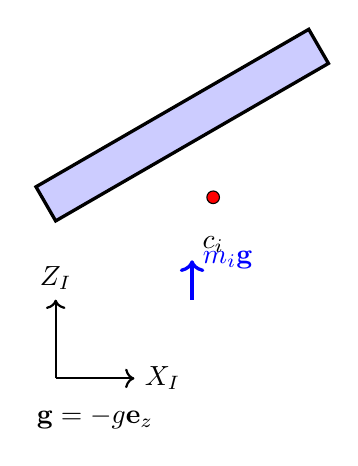
\begin{tikzpicture}[scale=1.0]
    % link i
    \draw[very thick,fill=blue!20,rotate=30] (0,0) rectangle (4,0.5);
    
    % centroid
    \draw[fill=red] (2,0.3) circle (0.08);
    \node at (2,-0.3) {$c_i$};
    
    % gravity
    \draw[->,very thick,blue] ({2*cos(30)},{-2+2*sin(30)}) -- ({2*cos(30)},{2*sin(30)-1.5}) node[right] {$m_i \mathbf{g}$};
    
    % inertial frame
    \draw[->,thick] (0,-2) -- (1,-2) node[right] {$X_I$};
    \draw[->,thick] (0,-2) -- (0,-1) node[above] {$Z_I$};
    
    % gravity direction
    \node at (0.5,-2.5) {$\mathbf{g} = -g\mathbf{e}_z$};
\end{tikzpicture}
\caption{Effect of gravity}
\end{figure}

The gravity in the inertial frame:
\begin{equation}
\mathbf{F}_{g,i} = m_i \mathbf{g} = \begin{bmatrix} 0 \\ 0 \\ -m_i g \end{bmatrix}
\label{eq:old-137}
\end{equation}

\textbf{Step 2: Gravitational Potential Energy}

\begin{equation}
V_g = \sum_{i=1}^{n} m_i g z_{c,i}
\label{eq:old-138}
\end{equation}

where $z_{c,i}$ is the vertical coordinate of the centroid of link $i$.

\textbf{Step 3: Generalized Force of Gravity}

Express the gravitational force first in the local frame of each link:
\begin{equation}
{}^{b,i}\mathbf{F}_{g,i} = {}_{I}^{b,i}\mathbf{R}\begin{bmatrix} 0 \\ 0 \\ -m_i g \end{bmatrix},
\qquad
\mathbf{W}_{g,i}^{(b,i)} :=
\begin{bmatrix}
{}^{b,i}\mathbf{F}_{g,i} \\
{}^{b,i}\mathbf{r}_{g,i} \times {}^{b,i}\mathbf{F}_{g,i}
\end{bmatrix}
\label{eq:old-139}
\end{equation}

Then map the local wrench into the system generalized force:
\begin{equation}
\mathbf{g}_g(\mathbf{q}) = \sum_{i=1}^{n} \bigl(\mathbf{J}_i^{(b,i)}(\mathbf{q})\bigr)^T \mathbf{W}_{g,i}^{(b,i)}
\label{eq:old-140}
\end{equation}
\newsymbols{$\mathbf{g}_g(\mathbf{q})$ is the generalized gravitational force, ${}^{b,i}\mathbf{r}_{g,i}$ is the position vector from the chosen body-fixed origin of link $i$ to its center of mass represented in $\Frame{b,i}$, and $\mathbf{W}_{g,i}^{(b,i)}$ is the corresponding local gravitational wrench.}

\subsection{Geometric Analysis of Buoyancy}

\textbf{Step 4: Archimedes' Principle}

The buoyant force equals the weight of the fluid displaced, acting at the center of buoyancy (geometric center of the displaced fluid); the corresponding pressure distribution and net upward resultant are included in Fig.~\ref{fig:hydrodynamic_cross_section}:
\begin{equation}
\mathbf{F}_{b,i} = \rho g V_i \mathbf{e}_z = \begin{bmatrix} 0 \\ 0 \\ \rho g V_i \end{bmatrix}
\label{eq:old-141}
\end{equation}

\textbf{Step 5: Gravitational Potential Energy of Buoyancy}

\begin{equation}
V_b = -\sum_{i=1}^{n} \rho g V_i z_{b,i}
\label{eq:old-142}
\end{equation}

The negative sign indicates that the potential energy of buoyancy is inversely proportional to the depth (the deeper the object, the more work is done by the buoyancy).

\textbf{Step 6: Generalized Force of Buoyancy}

\begin{equation}
\begin{aligned}
{}^{b,i}\mathbf{F}_{b,i} &= {}_{I}^{b,i}\mathbf{R}\begin{bmatrix} 0 \\ 0 \\ \rho g V_i \end{bmatrix}, \\
\mathbf{W}_{b,i}^{(b,i)} &:=
\begin{bmatrix}
{}^{b,i}\mathbf{F}_{b,i} \\
{}^{b,i}\mathbf{r}_{b,i} \times {}^{b,i}\mathbf{F}_{b,i}
\end{bmatrix}, \\
\mathbf{g}_b(\mathbf{q}) &= \sum_{i=1}^{n} \bigl(\mathbf{J}_i^{(b,i)}(\mathbf{q})\bigr)^T \mathbf{W}_{b,i}^{(b,i)}
\end{aligned}
\label{eq:old-143}
\end{equation}
\newsymbols{$\mathbf{g}_b(\mathbf{q})$ is the generalized buoyancy force, ${}^{b,i}\mathbf{r}_{b,i}$ is the position vector from the chosen body-fixed origin of link $i$ to its center of buoyancy represented in $\Frame{b,i}$, and $\mathbf{W}_{b,i}^{(b,i)}$ is the corresponding local buoyancy wrench.}

\subsection{Total Gravity-Buoyancy Terms}

\textbf{Step 7: Combine Gravity and Buoyancy}

\begin{equation}
\mathbf{N}({}_{b}^{I}\mathbf{R}, \mathbf{q}) = \mathbf{g}_g(\mathbf{q}) + \mathbf{g}_b(\mathbf{q})
\label{eq:old-144}
\end{equation}

Expanding:
\begin{align}
\mathbf{N}({}_{b}^{I}\mathbf{R}, \mathbf{q}) = \sum_{i=1}^{n} &\bigl(\mathbf{J}_i^{(b,i)}(\mathbf{q})\bigr)^T
\left(
\mathbf{W}_{g,i}^{(b,i)} + \mathbf{W}_{b,i}^{(b,i)}
\right)
\end{align}

\textbf{Step 8: Static Equilibrium Condition}

\begin{equation}
\mathbf{N}({}_{b}^{I}\mathbf{R}, \mathbf{q}) = \mathbf{0}
\end{equation}

For a neutrally buoyant system ($m_i = \rho V_i$) with the center of mass coinciding with the center of buoyancy (${}^{b,i}\mathbf{r}_{g,i} = {}^{b,i}\mathbf{r}_{b,i}$):
\begin{equation}
\mathbf{N}({}_{b}^{I}\mathbf{R}, \mathbf{q}) = \mathbf{0}
\end{equation}

\textbf{Step 9: Stability Analysis}

When the center of buoyancy $B$ is above the center of mass $G$, the system is stable. As illustrated in Fig.~\ref{fig:hydrodynamic_cross_section}, the separation between the buoyancy and gravity resultants generates a restoring moment when tilted.

\chapter{Actuator Models and Generalized Forces}

In this section and in the final assembled model, the actuator-generated generalized force is denoted by $\mathbf{u}$. The robot is driven by four propulsion motors mounted on the four links and by the six joint motors. Each propulsion motor drives one propulsion unit consisting of two counter-rotating screws, so the pair is modeled as one net axial thrust along the corresponding link while the reaction torque of the screws is canceled inside the unit.

\section{Distributed Propulsion Mapping}

\begin{equation}
\mathbf{u}_{\mathrm{prop}} = \mathbf{B}_{\mathrm{prop}}(\mathbf{q}) \mathbf{f}_{\mathrm{prop}},
\qquad
\mathbf{f}_{\mathrm{prop}} :=
\begin{bmatrix}
f_1 \\ f_2 \\ f_3 \\ f_4
\end{bmatrix}
\in \mathbb{R}^{4}
\label{eq:old-145}
\end{equation}
\newsymbols{$\mathbf{u}_{\mathrm{prop}}$ is the generalized force generated by the four distributed propulsion units. $\mathbf{B}_{\mathrm{prop}}(\mathbf{q})$ is the propulsion-allocation matrix. $\mathbf{f}_{\mathrm{prop}}$ collects the four axial thrust commands.}

\subsection{Geometric Analysis of Link-Mounted Propulsion Units}

\textbf{Step 1: Four propulsion units mounted on four links}

\begin{figure}[H]
\centering
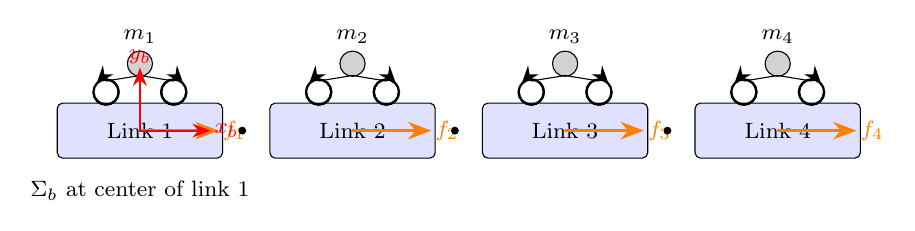
\begin{tikzpicture}[x=1cm,y=1cm,>=Stealth,line cap=round,line join=round,
    every node/.style={font=\footnotesize,inner sep=1pt}]
    \foreach \idx/\x/\lab in {1/0.0/{Link 1},2/2.7/{Link 2},3/5.4/{Link 3},4/8.1/{Link 4}} {
        \draw[rounded corners=2pt,fill=blue!12] (\x,0) rectangle ++(2.1,0.7);
        \node at (\x+1.05,0.35) {\lab};
        \draw[fill=gray!35] (\x+1.05,1.2) circle (0.16);
        \node[above] at (\x+1.05,1.42) {$m_{\idx}$};
        \draw[thick] (\x+0.62,0.84) circle (0.16);
        \draw[thick] (\x+1.48,0.84) circle (0.16);
        \draw (\x+1.05,1.05) -- (\x+0.62,0.98);
        \draw (\x+1.05,1.05) -- (\x+1.48,0.98);
        \draw[->,thick] (\x+0.46,0.84) arc[start angle=180,end angle=500,radius=0.16];
        \draw[->,thick] (\x+1.64,0.84) arc[start angle=0,end angle=-320,radius=0.16];
        \draw[->,very thick,orange] (\x+1.05,0.35) -- ++(1.0,0) node[right] {$f_{\idx}$};
    }
    \foreach \x in {2.35,5.05,7.75} {
        \fill (\x,0.35) circle (0.05);
    }
    \draw[->,thick,red] (1.05,0.35) -- (1.95,0.35) node[right] {$x_b$};
    \draw[->,thick,red] (1.05,0.35) -- (1.05,1.15) node[above] {$y_b$};
    \node[below] at (1.05,-0.25) {$\Sigma_b$ at center of link 1};
\end{tikzpicture}
\caption{Four link-mounted propulsion units with counter-rotating screw pairs}
\end{figure}

Each propulsion unit is installed at the centroid of its link. In the local coordinate system of link $i$, the two counter-rotating screws are modeled as one net axial force:
\begin{equation}
{}^{b,i}\mathbf{f}_{p_i} =
\begin{bmatrix}
f_i \\ 0 \\ 0
\end{bmatrix}
= \mathbf{e}_x f_i,
\qquad i = 1,2,3,4.
\end{equation}
\newsymbols{${}^{b,i}\mathbf{f}_{p_i}$ is the net thrust produced by the propulsion unit mounted on link $i$, expressed in the coordinate system of that link, and $m_i$ denotes the propulsion motor driving the screw pair on link $i$.}

\textbf{Step 2: Force expressed in the inertial frame}

Because the thrust is aligned with the longitudinal axis of link $i$,
\begin{equation}
{}^{I}\mathbf{f}_{p_i}
= {}_{b,i}^{I}\mathbf{R}\,{}^{b,i}\mathbf{f}_{p_i}
= {}_{b,i}^{I}\mathbf{R}\,\mathbf{e}_x f_i.
\end{equation}
The counter-rotating screw pair is assumed to cancel the internal reaction torque, so the propulsion unit contributes a pure force at the link centroid. This inertial-frame expression is equivalent to the local one above, but the generalized-force mapping below is carried out directly in $\Frame{b,i}$.

\textbf{Step 3: Generalized-force contribution of one propulsion unit}

Let $\mathbf{J}_i^{(b,i)}(\mathbf{q}) \in \mathbb{R}^{6\times12}$ be the local spatial Jacobian of link $i$ evaluated at the link centroid, and define the local propulsion wrench
\begin{equation}
\mathbf{W}_{p_i}^{(b,i)}
:=
\begin{bmatrix}
{}^{b,i}\mathbf{f}_{p_i} \\
\mathbf{0}_3
\end{bmatrix}
=
\begin{bmatrix}
\mathbf{e}_x \\
\mathbf{0}_3
\end{bmatrix}
f_i.
\end{equation}
Then the generalized force induced by the propulsion unit on link $i$ follows from virtual work:
\begin{equation}
\mathbf{u}_{p_i}
= \bigl(\mathbf{J}_i^{(b,i)}(\mathbf{q})\bigr)^T \mathbf{W}_{p_i}^{(b,i)}
= \mathbf{b}_{p_i}(\mathbf{q}) f_i,
\end{equation}
where
\begin{equation}
\mathbf{b}_{p_i}(\mathbf{q})
:=
\bigl(\mathbf{J}_i^{(b,i)}(\mathbf{q})\bigr)^T
\begin{bmatrix}
\mathbf{e}_x \\
\mathbf{0}_3
\end{bmatrix}
\in \mathbb{R}^{12}.
\end{equation}
\newsymbols{$\mathbf{u}_{p_i}$ is the generalized force contribution of the propulsion unit on link $i$, $\mathbf{W}_{p_i}^{(b,i)}$ is the corresponding local propulsion wrench, and $\mathbf{b}_{p_i}(\mathbf{q})$ is the propulsion-allocation column obtained from the local Jacobian.}

\textbf{Step 4: Four-unit propulsion allocation matrix}

Summing the four link-mounted propulsion contributions gives
\begin{equation}
\mathbf{u}_{\mathrm{prop}}
= \sum_{i=1}^{4} \mathbf{u}_{p_i}
= \sum_{i=1}^{4} \mathbf{b}_{p_i}(\mathbf{q}) f_i
=
\begin{bmatrix}
\mathbf{b}_{p_1}(\mathbf{q}) &
\mathbf{b}_{p_2}(\mathbf{q}) &
\mathbf{b}_{p_3}(\mathbf{q}) &
\mathbf{b}_{p_4}(\mathbf{q})
\end{bmatrix}
\mathbf{f}_{\mathrm{prop}}.
\end{equation}
Therefore
\begin{equation}
\boxed{
\mathbf{B}_{\mathrm{prop}}(\mathbf{q})
=
\begin{bmatrix}
\mathbf{b}_{p_1}(\mathbf{q}) &
\mathbf{b}_{p_2}(\mathbf{q}) &
\mathbf{b}_{p_3}(\mathbf{q}) &
\mathbf{b}_{p_4}(\mathbf{q})
\end{bmatrix}
\in \mathbb{R}^{12\times4}
}.
\end{equation}
\formulaannotation{Equation~\eqref{eq:old-145} maps the four link-mounted propulsion forces into the generalized force of the full underwater multibody system.}

\section{Joint Actuation}

\begin{equation}
\boldsymbol{\tau} = \begin{bmatrix} \tau_{1} \\ \tau_{2} \\ \tau_{3} \\ \tau_{4} \\ \tau_{5} \\ \tau_{6} \end{bmatrix}
\label{eq:old-146}
\end{equation}

The vector $\boldsymbol{\tau}$ collects the six motor torques applied to the six internal joint coordinates and enters the system generalized force through the selector matrix $\mathbf{S}_{\tau}$.

\section{Total Generalized Force}

\begin{equation}
\mathbf{u}
= \mathbf{u}_{\mathrm{prop}} + \mathbf{S}_{\tau}\boldsymbol{\tau}
= \mathbf{B}_{\mathrm{act}}(\mathbf{q})\mathbf{a},
\qquad
\mathbf{S}_{\tau}
:=
\begin{bmatrix}
\mathbf{0}_{6\times6} \\
\mathbf{I}_{6\times6}
\end{bmatrix},
\qquad
\mathbf{a}
:=
\begin{bmatrix}
\mathbf{f}_{\mathrm{prop}} \\
\boldsymbol{\tau}
\end{bmatrix}
\label{eq:old-147}
\end{equation}
\begin{equation}
\mathbf{B}_{\mathrm{act}}(\mathbf{q})
:=
\begin{bmatrix}
\mathbf{B}_{\mathrm{prop}}(\mathbf{q}) & \mathbf{S}_{\tau}
\end{bmatrix}
\in \mathbb{R}^{12\times10}.
\end{equation}
\newsymbols{$\mathbf{S}_{\tau}$ injects the six joint torques into the generalized-force vector, $\mathbf{a}$ is the complete actuator command vector, and $\mathbf{B}_{\mathrm{act}}(\mathbf{q})$ is the combined actuator-allocation matrix for the four propulsion motors and six joint motors.}

\subsection{Derivation}

The total generalized force consists of two parts:
\begin{enumerate}
    \item The distributed propulsion contribution from the four link-mounted propulsion units: $\mathbf{u}_{\mathrm{prop}} = \mathbf{B}_{\mathrm{prop}}(\mathbf{q}) \mathbf{f}_{\mathrm{prop}}$
    \item The joint-motor torques injected through $\mathbf{S}_{\tau}\boldsymbol{\tau}$
\end{enumerate}

Written in block matrix form:
\begin{equation}
\mathbf{u}
=
\begin{bmatrix}
\mathbf{B}_{\mathrm{prop}}(\mathbf{q}) & \mathbf{S}_{\tau}
\end{bmatrix}
\begin{bmatrix}
\mathbf{f}_{\mathrm{prop}} \\
\boldsymbol{\tau}
\end{bmatrix}.
\end{equation}
\formulaannotation{Equation~\eqref{eq:old-147} collects the four propulsion-motor commands and the six joint torques into one 10-dimensional actuator vector.}

\chapter{Complete Dynamic Equations}

\section{Complete Newton--Euler Dynamic Equations}

Chapter~7 collects the inertia, velocity-dependent, damping, restoring, and actuator terms derived in Chapters~4--6 into the final control-ready form. Incorporating those terms, the complete dynamic equation for underwater multibody robots is:

\begin{equation}
\boxed{
\mathbf{M}(\mathbf{q})\dot{\boldsymbol{\zeta}} + \mathbf{C}(\mathbf{q},\boldsymbol{\zeta})\boldsymbol{\zeta} + \mathbf{D}(\mathbf{q},\boldsymbol{\zeta})\boldsymbol{\zeta} + \mathbf{N}({}_{b}^{I}\mathbf{R}, \mathbf{q}) = \mathbf{u} = \begin{bmatrix}
\mathbf{B}_{\mathrm{prop}}(\mathbf{q}) & \mathbf{S}_{\tau}
\end{bmatrix} \begin{bmatrix}
\mathbf{f}_{\mathrm{prop}} \\ \boldsymbol{\tau}
\end{bmatrix}
}
\label{eq:old-148}
\end{equation}

Equation~\eqref{eq:old-148} is the complete floating-base underwater multibody model used below. Its left-hand side collects the inertia, velocity-dependent, damping, and restoring generalized forces in the quasi-velocity coordinates $\boldsymbol{\zeta}$. The right-hand side is the realized generalized force generated by the four propulsion units and six joint motors through $\mathbf{B}_{\mathrm{act}}(\mathbf{q})$. Here $\mathbf{M}$ includes both rigid-body inertia and added mass, $\mathbf{C}\boldsymbol{\zeta}$ is the Newton--Euler velocity-dependent product term, $\mathbf{D}\boldsymbol{\zeta}$ maps local hydrodynamic damping wrenches through the link Jacobians, and $\mathbf{N}$ is the gravity-buoyancy restoring contribution.

\section{Special-Case Remarks}

The following reductions should be read as special-case models or constrained subsystems, not as automatic algebraic deletions of terms. Whenever one of them is enforced as a constraint inside the full three-dimensional model, the initial condition and the applied generalized forces must be compatible with that constraint and preserve it over time.

\paragraph{Planar motion.}
For a \emph{minimal} planar reduction, the floating base contributes two translations and one yaw angle, and each of the three physical joints contributes one in-plane relative angle. Therefore the present four-link chain reduces to a 6-dimensional generalized coordinate vector. If one instead keeps the full three-dimensional model, planar motion is obtained as a constrained subsystem by setting the out-of-plane coordinates and the corresponding generalized forces to zero. In that constrained interpretation, planar motion is not obtained merely by deleting terms: the initial state must already satisfy the planar constraint and the applied inputs must preserve that constraint along the motion.

\paragraph{Neutral buoyancy.}
When $m_i = \rho V_i$ and the center of mass coincides with the center of buoyancy for every link, the restoring term vanishes:
\begin{equation}
\mathbf{N}({}_{b}^{I}\mathbf{R},\mathbf{q}) = \mathbf{0}.
\end{equation}
This does \emph{not} mean that the gravitational acceleration is zero; it means that gravity and buoyancy cancel in the generalized-force balance.

\paragraph{Neglecting fluid effects.}
When all fluid effects are neglected ($\mathbf{M}_A = \mathbf{0}$, $\mathbf{D} = \mathbf{0}$, no buoyancy), the system reduces to a land-based multibody system:
\begin{equation}
\mathbf{M}_{\text{RB}}(\mathbf{q})\dot{\boldsymbol{\zeta}} + \mathbf{C}_{\text{RB}}(\mathbf{q},\boldsymbol{\zeta})\boldsymbol{\zeta} + \mathbf{g}_g(\mathbf{q}) = \mathbf{u}
\end{equation}
where $\mathbf{C}_{\text{RB}}$ denotes the rigid-body part of the Coriolis--centripetal matrix obtained by deleting the added-mass terms from $\mathbf{C}(\mathbf{q},\boldsymbol{\zeta})$. In this limit, the restoring term of the full underwater model degenerates to the pure gravity term $\mathbf{g}_g(\mathbf{q})$.

\clearpage
\chapter{Dynamic Front-Unit-Following Control}

This section combines a geometric front-unit-following construction with the full underwater Newton--Euler model of Eq.~\eqref{eq:old-148}. The horizontal motion of the leading reference point and the yaw-chain geometry are generated kinematically, the out-of-plane coordinates are stabilized independently, and the required actuator command is then recovered through inverse dynamics and actuator allocation.

Throughout this section, the six internal coordinates are ordered sequentially as $(\theta_1,\theta_2,\theta_3,\theta_4,\theta_5,\theta_6)$, with pitch coordinates $(\theta_1,\theta_3,\theta_5)$ and yaw coordinates $(\theta_2,\theta_4,\theta_6)$. Let $P_H$ denote the leading reference point used by the projected front-following geometry, and let $\psi_p$ denote the heading angle of the horizontal projection of the longitudinal axis of link~1. Under the link-1-centered convention adopted here, the positive $x$-axis points from $P_H$ toward the downstream joints, which is why the later geometry uses ${}^{b}\mathbf{r}_H=-L_{1,1}\mathbf{e}_x$.

\section{Projected Output Coordinates}

We first split the controlled variables into a projected front-following part and an out-of-plane stabilization part. The leading-point state, the yaw-chain state, and the auxiliary state are defined by
\begin{equation}
\mathbf{y} =
\begin{bmatrix}
\boldsymbol{\xi}_p \\
\boldsymbol{\phi}_y \\
\boldsymbol{\eta}
\end{bmatrix},
\quad
\boldsymbol{\xi}_p =
\begin{bmatrix}
x_p \\
y_p \\
\psi_p
\end{bmatrix},
\quad
\boldsymbol{\phi}_y =
\begin{bmatrix}
\theta_{2} \\
\theta_{4} \\
\theta_{6}
\end{bmatrix},
\quad
\boldsymbol{\eta} =
\begin{bmatrix}
z_b \\
\varphi_b \\
\vartheta_b \\
\theta_{1} \\
\theta_{3} \\
\theta_{5}
\end{bmatrix}
\in \mathbb{R}^{6}.
\label{eq:old-149}
\end{equation}
\newsymbols{$\mathbf{y}$ is the complete output vector used by the front-following controller, $P_H$ is the leading reference point used by the front-unit-following controller, $\boldsymbol{\xi}_p$ is the leading-point state, $\boldsymbol{\phi}_y$ collects the three yaw coordinates, and $\boldsymbol{\eta}$ collects the out-of-plane coordinates to be independently stabilized.}
\noindent
Here $x_p$ and $y_p$ are the inertial-frame horizontal coordinates of $P_H$, $\psi_p$ is the heading angle of the horizontal projection of the longitudinal axis of link~1, $\theta_{2},\theta_{4},\theta_{6}$ are the three yaw coordinates, and $z_b,\varphi_b,\vartheta_b,\theta_{1},\theta_{3},\theta_{5}$ are respectively the base vertical position, base roll, base pitch, and the three pitch coordinates.
\formulaannotation{Equation~\eqref{eq:old-149} partitions the controller outputs into horizontal front-following coordinates and auxiliary out-of-plane coordinates.}

For the present four-link robot, the generalized velocity is ordered as
\begin{equation}
\boldsymbol{\zeta} =
\left[
\begin{array}{cccccccccccc}
u_b &
v_b &
w_b &
p_b &
q_b &
r_b &
\dot{\theta}_{1} &
\dot{\theta}_{2} &
\dot{\theta}_{3} &
\dot{\theta}_{4} &
\dot{\theta}_{5} &
\dot{\theta}_{6}
\end{array}
\right]^{T}.
\end{equation}
\begin{equation}
\boldsymbol{\nu}_{\mathrm{lin},b} :=
\begin{bmatrix}
u_b \\ v_b \\ w_b
\end{bmatrix},
\qquad
\boldsymbol{\omega}_b :=
\begin{bmatrix}
p_b \\ q_b \\ r_b
\end{bmatrix},
\qquad
\dot{\boldsymbol{\theta}} :=
\begin{bmatrix}
\dot{\theta}_{1} & \dot{\theta}_{2} & \dot{\theta}_{3} & \dot{\theta}_{4} & \dot{\theta}_{5} & \dot{\theta}_{6}
\end{bmatrix}^{T}.
\end{equation}
\newsymbols{$u_b,v_b,w_b$ are the components of the base linear velocity in the base frame, $p_b,q_b,r_b$ are the components of the base angular velocity in the base frame, $\boldsymbol{\nu}_{\mathrm{lin},b}$ is the base linear-velocity vector, $\boldsymbol{\omega}_b$ is the base angular-velocity vector, and $\dot{\boldsymbol{\theta}}$ collects all joint rates.}

Let $\mathbf{e}_x = [1,0,0]^T$, $\mathbf{e}_y = [0,1,0]^T$, and $\mathbf{e}_z = [0,0,1]^T$ denote the inertial basis vectors. The inertial position of the leading reference point and the projected heading are defined by
\begin{equation}
{}^{I}\mathbf{p}_H =
{}^{I}\mathbf{p}_b +
{}_{b}^{I}\mathbf{R}\,{}^{b}\mathbf{r}_H(\mathbf{q}),
\qquad
x_p = \mathbf{e}_x^T {}^{I}\mathbf{p}_H,
\qquad
y_p = \mathbf{e}_y^T {}^{I}\mathbf{p}_H.
\end{equation}
\begin{equation}
{}^{I}\mathbf{t}_H =
{}_{b}^{I}\mathbf{R}\,{}^{b}\mathbf{t}_H(\mathbf{q}),
\qquad
\psi_p =
\operatorname{atan2}
\bigl(
\mathbf{e}_y^T {}^{I}\mathbf{t}_H,
\mathbf{e}_x^T {}^{I}\mathbf{t}_H
\bigr).
\end{equation}
Here ${}^{b}\mathbf{r}_H(\mathbf{q})$ is the vector from the base origin to $P_H$ expressed in the base frame, and ${}^{b}\mathbf{t}_H(\mathbf{q})$ is the corresponding unit tangent direction of the front link in the base frame.
\newsymbols{${}^{I}\mathbf{p}_H$ is the inertial position of the leading reference point, ${}^{I}\mathbf{p}_b$ is the inertial position of the floating-base origin, ${}^{b}\mathbf{r}_H(\mathbf{q})$ is the base-frame vector from the base origin to the leading point, ${}^{I}\mathbf{t}_H$ is the inertial unit tangent of the front link, and ${}^{b}\mathbf{t}_H(\mathbf{q})$ is the same tangent represented in the base frame.}

To make the four-link geometry explicit, the controller uses the front-link-centered convention stated in the front matter: the floating base frame $\Sigma_b$ is attached to the center of link~1 and its positive $x$-axis points from $P_H$ toward the downstream joints. Let
\begin{equation}
\mathbf{R}_{y}(\beta) =
\begin{bmatrix}
\cos \beta & 0 & \sin \beta \\
0 & 1 & 0 \\
-\sin \beta & 0 & \cos \beta
\end{bmatrix},
\qquad
\mathbf{R}_{z}(\gamma) =
\begin{bmatrix}
\cos \gamma & -\sin \gamma & 0 \\
\sin \gamma & \cos \gamma & 0 \\
0 & 0 & 1
\end{bmatrix}.
\end{equation}
\newsymbols{$\mathbf{R}_y(\beta)$ is the rotation matrix for a pitch rotation $\beta$ about the body $y$-axis, and $\mathbf{R}_z(\gamma)$ is the rotation matrix for a yaw rotation $\gamma$ about the body $z$-axis.}

The base frame now coincides with link 1, so the link orientations satisfy the recursion
\begin{equation}
\begin{aligned}
{}_{1}^{b}\mathbf{R} &= \mathbf{I}_3, \\
{}_{2}^{b}\mathbf{R}
&= \mathbf{R}_{y}(\theta_{1}) \mathbf{R}_{z}(\theta_{2}), \\
{}_{3}^{b}\mathbf{R}
&= {}_{2}^{b}\mathbf{R}\,\mathbf{R}_{y}(\theta_{3}) \mathbf{R}_{z}(\theta_{4}), \\
{}_{4}^{b}\mathbf{R}
&= {}_{3}^{b}\mathbf{R}\,\mathbf{R}_{y}(\theta_{5}) \mathbf{R}_{z}(\theta_{6}).
\end{aligned}
\end{equation}
Hence the longitudinal axes of the four links, expressed in $\Sigma_b$, are
\begin{equation}
{}^{b}\mathbf{e}_{x,i} = {}_{i}^{b}\mathbf{R}\,\mathbf{e}_x,
\qquad i = 1,2,3,4,
\qquad
{}^{b}\mathbf{t}_H(\mathbf{q}) = {}^{b}\mathbf{e}_{x,1}.
\end{equation}

Using the same indexed geometry as the kinematic chapter, let $L_{i,1}$ be the distance from the centroid of link $i$ to the leading reference side and let $L_{i,2}$ be the distance from the centroid to the downstream joint side, with $\Lambda_i := L_{i,1}+L_{i,2}$ denoting the full length of link $i$. Starting from the base origin at the center of link~1 gives the leading reference point and the three joint locations
\begin{equation}
\begin{aligned}
{}^{b}\mathbf{r}_H(\mathbf{q}) =
-L_{1,1}\,{}^{b}\mathbf{e}_{x,1},
\qquad
{}^{b}\mathbf{r}_{J_1} = L_{1,2}\,{}^{b}\mathbf{e}_{x,1},
\\
{}^{b}\mathbf{r}_{J_2} = L_{1,2}\,{}^{b}\mathbf{e}_{x,1} + \Lambda_2\,{}^{b}\mathbf{e}_{x,2},
\qquad
{}^{b}\mathbf{r}_{J_3} = L_{1,2}\,{}^{b}\mathbf{e}_{x,1} + \Lambda_2\,{}^{b}\mathbf{e}_{x,2} + \Lambda_3\,{}^{b}\mathbf{e}_{x,3}.
\end{aligned}
\end{equation}
\newsymbols{$L_{i,1}$ is the distance from the centroid of link $i$ to the leading reference side, $L_{i,2}$ is the distance from the centroid to the downstream joint side, $\Lambda_i$ is the full length of link $i$, and ${}^{b}\mathbf{r}_{J_k}$ is the position of joint $k$ in the base frame.}

Subtracting each joint position from the leading-point position yields the corresponding lever-arm vectors
\begin{equation}
\begin{aligned}
{}^{b}\boldsymbol{\rho}_1
&= {}^{b}\mathbf{r}_H - {}^{b}\mathbf{r}_{J_1}
= -(L_{1,1}+L_{1,2})\,{}^{b}\mathbf{e}_{x,1}, \\
{}^{b}\boldsymbol{\rho}_2
&= {}^{b}\mathbf{r}_H - {}^{b}\mathbf{r}_{J_2}
= -(L_{1,1}+L_{1,2})\,{}^{b}\mathbf{e}_{x,1} - \Lambda_2\,{}^{b}\mathbf{e}_{x,2}, \\
{}^{b}\boldsymbol{\rho}_3
&= {}^{b}\mathbf{r}_H - {}^{b}\mathbf{r}_{J_3}
= -(L_{1,1}+L_{1,2})\,{}^{b}\mathbf{e}_{x,1} - \Lambda_2\,{}^{b}\mathbf{e}_{x,2} - \Lambda_3\,{}^{b}\mathbf{e}_{x,3}.
\end{aligned}
\end{equation}
\newsymbols{${}^{b}\boldsymbol{\rho}_k$ is the vector from joint $k$ to the leading point, expressed in the base frame.}
\formulaannotation{The preceding geometry formulas express the leading point and all joint-to-leading-point lever arms entirely in terms of link directions.}

With the pitch-first convention used above, the instantaneous pitch and yaw axes of joint $k$ are
\begin{equation}
{}^{b}\mathbf{a}_{k,p} = {}_{k}^{b}\mathbf{R}\,\mathbf{e}_y,
\qquad
{}^{b}\mathbf{a}_{k,y} = {}_{k}^{b}\mathbf{R}\,\mathbf{R}_{y}(\theta_{2k-1})\,\mathbf{e}_z,
\qquad
k = 1,2,3.
\end{equation}
These are the rotation axes associated with the ordered coordinates $(\theta_{2k-1},\theta_{2k})$ of each physical joint.
\newsymbols{${}^{b}\mathbf{a}_{k,p}$ is the pitch axis of joint $k$ in the base frame, and ${}^{b}\mathbf{a}_{k,y}$ is the yaw axis of joint $k$ in the base frame.}

For the present four-link chain, the recursive geometry above can be written componentwise. Introduce the shorthand
\begin{equation}
c_j := \cos \theta_j,
\qquad
s_j := \sin \theta_j,
\qquad
j = 1,\ldots,6.
\end{equation}
\newsymbols{$c_j$ and $s_j$ are abbreviations for the cosine and sine of the sequential joint coordinate $\theta_j$.}

Because link 1 coincides with the base frame, the front-link direction and the first joint axes are
\begin{equation}
{}^{b}\mathbf{e}_{x,1} = \mathbf{e}_x =
\begin{bmatrix}
1 \\ 0 \\ 0
\end{bmatrix}.
\end{equation}
\begin{equation}
{}^{b}\mathbf{a}_{1,p} = \mathbf{e}_y =
\begin{bmatrix}
0 \\ 1 \\ 0
\end{bmatrix},
\qquad
{}^{b}\mathbf{a}_{1,y}
= \mathbf{R}_{y}(\theta_{1})\mathbf{e}_z
=
\begin{bmatrix}
s_{1} \\ 0 \\ c_{1}
\end{bmatrix}.
\end{equation}
For the downstream links, define the intermediate orientations
\begin{equation}
\mathbf{R}_{21} := \mathbf{R}_{y}(\theta_{1})\mathbf{R}_{z}(\theta_{2}),
\qquad
\mathbf{R}_{32} := \mathbf{R}_{21}\mathbf{R}_{y}(\theta_{3})\mathbf{R}_{z}(\theta_{4}).
\end{equation}
\begin{equation}
{}^{b}\mathbf{e}_{x,2}
= \mathbf{R}_{21}\mathbf{e}_x
=
\begin{bmatrix}
c_{1}c_{2} \\
s_{2} \\
-s_{1}c_{2}
\end{bmatrix}.
\end{equation}
\begin{equation}
{}^{b}\mathbf{a}_{2,p}
= \mathbf{R}_{21}\mathbf{e}_y
=
\begin{bmatrix}
-c_{1}s_{2} \\
c_{2} \\
s_{1}s_{2}
\end{bmatrix}.
\end{equation}
\begin{equation}
\begin{aligned}
{}^{b}\mathbf{a}_{2,y} &= \mathbf{R}_{21}\mathbf{R}_y(\theta_{3})\mathbf{e}_z, \\
{}^{b}\mathbf{e}_{x,3} &= \mathbf{R}_{32}\mathbf{e}_x, \\
{}^{b}\mathbf{a}_{3,p} &= \mathbf{R}_{32}\mathbf{e}_y, \\
{}^{b}\mathbf{a}_{3,y} &= \mathbf{R}_{32}\mathbf{R}_y(\theta_{5})\mathbf{e}_z, \\
{}^{b}\mathbf{e}_{x,4} &= {}_{4}^{b}\mathbf{R}\,\mathbf{e}_x.
\end{aligned}
\end{equation}
Expanding these products gives the complete trigonometric component formulas whenever a fully explicit expression is needed, but the recursive matrix forms above already provide all geometric ingredients required by the controller derivation.
\newsymbols{$\mathbf{R}_{21}$ and $\mathbf{R}_{32}$ are the intermediate orientations of links 2 and 3 represented in the base frame under the link-1-centered convention.}
\formulaannotation{The component formulas above make the link-1-centered geometry explicit while preserving the same pitch-first joint convention used throughout the document.}

We next derive the Jacobian that maps the generalized velocity to the rates of the controlled outputs. Differentiating the leading-point position gives
\begin{align}
{}^{I}\dot{\mathbf{p}}_H
&= {}^{I}\dot{\mathbf{p}}_b + {}_{b}^{I}\dot{\mathbf{R}}\,{}^{b}\mathbf{r}_H \\
&= {}_{b}^{I}\mathbf{R}\boldsymbol{\nu}_{\mathrm{lin},b} + {}_{b}^{I}\mathbf{R}\bigl(\boldsymbol{\omega}_b \times {}^{b}\mathbf{r}_H\bigr) \\
&= {}_{b}^{I}\mathbf{R}
\left(
\boldsymbol{\nu}_{\mathrm{lin},b} - ({}^{b}\mathbf{r}_H)^\wedge \boldsymbol{\omega}_b
\right),
\end{align}
where $\mathbf{a} \times \mathbf{b} = \mathbf{a}^\wedge \mathbf{b}$ has been used. Under the link-1-centered convention, ${}^{b}\mathbf{r}_H = -L_{1,1}\mathbf{e}_x$ is constant in the base frame, so the leading-point position has no direct joint-rate contribution. Therefore
\begin{equation}
\mathbf{J}_{H,p}(\mathbf{q}) =
\begin{bmatrix}
{}_{b}^{I}\mathbf{R}
\begin{bmatrix}
\mathbf{I}_3 & -({}^{b}\mathbf{r}_H(\mathbf{q}))^\wedge
\end{bmatrix}
&
\mathbf{0}_{3\times6}
\end{bmatrix},
\end{equation}
with
\begin{equation}
\mathbf{J}_{H,\theta}^{(p)}(\mathbf{q}) = \mathbf{0}_{3\times6}.
\end{equation}
Hence the projected leading-point position is driven only by floating-base translation and rotation; the downstream joints enter the controlled output through $\boldsymbol{\phi}_y$ and $\boldsymbol{\eta}$ instead.

For the front-link tangent vector,
\begin{align}
{}^{I}\dot{\mathbf{t}}_H
&= {}_{b}^{I}\dot{\mathbf{R}}\,{}^{b}\mathbf{t}_H \\
&= {}_{b}^{I}\mathbf{R}\bigl(\boldsymbol{\omega}_b \times {}^{b}\mathbf{t}_H\bigr) \\
&= {}_{b}^{I}\mathbf{R}
\left(
-({}^{b}\mathbf{t}_H)^\wedge \boldsymbol{\omega}_b
\right),
\end{align}
where
\begin{equation}
\mathbf{J}_{H,\theta}^{(t)}(\mathbf{q}) = \mathbf{0}_{3\times6},
\qquad
{}^{b}\mathbf{t}_H(\mathbf{q}) = \mathbf{e}_x.
\end{equation}
Hence
\begin{equation}
\mathbf{J}_{H,t}(\mathbf{q}) =
\begin{bmatrix}
\mathbf{0}_{3\times3} &
-{}_{b}^{I}\mathbf{R}({}^{b}\mathbf{t}_H(\mathbf{q}))^\wedge &
\mathbf{0}_{3\times6}
\end{bmatrix},
\end{equation}

The projected heading is $\psi_p = \operatorname{atan2}(t_{Hy},t_{Hx})$ with
\begin{equation}
t_{Hx} := \mathbf{e}_x^T {}^{I}\mathbf{t}_H,
\qquad
t_{Hy} := \mathbf{e}_y^T {}^{I}\mathbf{t}_H.
\end{equation}
Therefore
\begin{align}
\dot{\psi}_p
&=
\frac{t_{Hx}\dot{t}_{Hy} - t_{Hy}\dot{t}_{Hx}}{t_{Hx}^{2} + t_{Hy}^{2}} \\
&=
\frac{1}{t_{Hx}^{2} + t_{Hy}^{2}}
\begin{bmatrix}
-t_{Hy} & t_{Hx} & 0
\end{bmatrix}
{}^{I}\dot{\mathbf{t}}_H \\
&=
\frac{1}{t_{Hx}^{2} + t_{Hy}^{2}}
\begin{bmatrix}
-t_{Hy} & t_{Hx} & 0
\end{bmatrix}
\mathbf{J}_{H,t}(\mathbf{q})\boldsymbol{\zeta}.
\end{align}
Thus
\begin{equation}
\mathbf{j}_{\psi}(\mathbf{q}) =
\frac{1}{t_{Hx}^{2} + t_{Hy}^{2}}
\begin{bmatrix}
-t_{Hy} & t_{Hx} & 0
\end{bmatrix}
\mathbf{J}_{H,t}(\mathbf{q}).
\end{equation}

The leading-point-state Jacobian is therefore
\begin{equation}
\mathbf{J}_p(\mathbf{q}) =
\begin{bmatrix}
\mathbf{e}_x^T \mathbf{J}_{H,p}(\mathbf{q}) \\
\mathbf{e}_y^T \mathbf{J}_{H,p}(\mathbf{q}) \\
\mathbf{j}_{\psi}(\mathbf{q})
\end{bmatrix}.
\end{equation}

\begin{equation}
\mathbf{S}_y =
\begin{bmatrix}
\mathbf{0}_{3\times6} & \mathbf{E}_y
\end{bmatrix},
\qquad
\mathbf{S}_p =
\begin{bmatrix}
\mathbf{0}_{3\times6} & \mathbf{E}_p
\end{bmatrix},
\end{equation}
with
\begin{equation}
\mathbf{E}_y =
\begin{bmatrix}
0 & 1 & 0 & 0 & 0 & 0 \\
0 & 0 & 0 & 1 & 0 & 0 \\
0 & 0 & 0 & 0 & 0 & 1
\end{bmatrix},
\qquad
\mathbf{E}_p =
\begin{bmatrix}
1 & 0 & 0 & 0 & 0 & 0 \\
0 & 0 & 1 & 0 & 0 & 0 \\
0 & 0 & 0 & 0 & 1 & 0
\end{bmatrix}.
\end{equation}
The selector $\mathbf{S}_y$ extracts the yaw rates from $\boldsymbol{\zeta}$, and $\mathbf{S}_p$ extracts the pitch rates.

For the auxiliary variables, the vertical coordinate obeys
\begin{equation}
\dot{z}_b = \mathbf{e}_z^T {}^{I}\dot{\mathbf{p}}_b = \mathbf{e}_z^T {}_{b}^{I}\mathbf{R}\,\boldsymbol{\nu}_{\mathrm{lin},b}.
\end{equation}
Under the ZYX Euler-angle convention, the roll and pitch rates satisfy
\begin{equation}
\mathbf{T}_{rp}(\varphi_b,\vartheta_b) =
\begin{bmatrix}
1 & \sin \varphi_b \tan \vartheta_b & \cos \varphi_b \tan \vartheta_b \\
0 & \cos \varphi_b & -\sin \varphi_b
\end{bmatrix},
\end{equation}
which maps the body angular velocity $[p_b,q_b,r_b]^T$ to $[\dot{\varphi}_b,\dot{\vartheta}_b]^T$ under the ZYX Euler-angle convention. Together with the pitch-rate selector $\mathbf{S}_p$, this gives
\begin{equation}
\mathbf{T}_{\eta}(\mathbf{q}) =
\begin{bmatrix}
\mathbf{e}_z^T {}_{b}^{I}\mathbf{R} & \mathbf{0}_{1\times3} & \mathbf{0}_{1\times6} \\
\mathbf{0}_{2\times3} & \mathbf{T}_{rp}(\varphi_b,\vartheta_b) & \mathbf{0}_{2\times6} \\
\mathbf{0}_{3\times3} & \mathbf{0}_{3\times3} & \mathbf{E}_p
\end{bmatrix}.
\end{equation}
\newsymbols{$\mathbf{J}_{H,\theta}^{(p)}(\mathbf{q})$ is the joint Jacobian of the leading-point position in the base frame, $\mathbf{J}_{H,\theta}^{(t)}(\mathbf{q})$ is the joint Jacobian of the front-link tangent direction in the base frame, $\mathbf{J}_{H,p}(\mathbf{q})$ maps $\boldsymbol{\zeta}$ to the leading-point velocity, $\mathbf{J}_{H,t}(\mathbf{q})$ maps $\boldsymbol{\zeta}$ to the front-link tangent velocity, $\mathbf{j}_{\psi}(\mathbf{q})$ maps $\boldsymbol{\zeta}$ to the projected heading rate, $\mathbf{J}_p(\mathbf{q})$ maps $\boldsymbol{\zeta}$ to the leading-point-state rate, $\mathbf{S}_y$ and $\mathbf{S}_p$ are the yaw-rate and pitch-rate selector matrices, $\mathbf{T}_{rp}(\varphi_b,\vartheta_b)$ is the roll-pitch kinematic map under the ZYX Euler-angle convention, $\mathbf{T}_{\eta}(\mathbf{q})$ maps $\boldsymbol{\zeta}$ to the auxiliary-state rate $\dot{\boldsymbol{\eta}}$, $t_{Hx}$ and $t_{Hy}$ are the $x$- and $y$-components of the projected front-link tangent, and $\mathbf{E}_y,\mathbf{E}_p$ select the yaw and pitch joint rates, respectively.}

Collecting $\dot{\boldsymbol{\xi}}_p = \mathbf{J}_p(\mathbf{q})\boldsymbol{\zeta}$, $\dot{\boldsymbol{\phi}}_y = \mathbf{S}_y\boldsymbol{\zeta}$, and $\dot{\boldsymbol{\eta}} = \mathbf{T}_{\eta}(\mathbf{q})\boldsymbol{\zeta}$ gives
\begin{equation}
\dot{\mathbf{y}} =
\begin{bmatrix}
\dot{\boldsymbol{\xi}}_p \\
\dot{\boldsymbol{\phi}}_y \\
\dot{\boldsymbol{\eta}}
\end{bmatrix}
=
\mathbf{A}_{\mathrm{ff}}(\mathbf{q}) \boldsymbol{\zeta},
\qquad
\mathbf{A}_{\mathrm{ff}}(\mathbf{q}) :=
\begin{bmatrix}
\mathbf{J}_p(\mathbf{q}) \\
\mathbf{S}_y \\
\mathbf{T}_{\eta}(\mathbf{q})
\end{bmatrix}
\in \mathbb{R}^{12 \times 12}.
\label{eq:old-150}
\end{equation}
\newsymbols{$\mathbf{A}_{\mathrm{ff}}(\mathbf{q})$ is the front-following output Jacobian.}
\formulaannotation{Equation~\eqref{eq:old-150} states that the chosen controller outputs are related linearly to the generalized velocity by a square output Jacobian.}

\paragraph{Local validity conditions.}
Define the local operating set
\begin{equation}
\Omega :=
\left\{
\mathbf{q}:\ 
t_{Hx}^{2}+t_{Hy}^{2}>0,\quad
\cos\vartheta_b \neq 0,\quad
\det \mathbf{A}_{\mathrm{ff}}(\mathbf{q}) \neq 0
\right\}.
\end{equation}
The first condition keeps the projected heading derivative well defined, the second avoids the ZYX roll-pitch singularity in $\mathbf{T}_{rp}$, and the third is the explicit nonsingularity assumption for the square output Jacobian. Therefore the mapping $\dot{\mathbf{y}}=\mathbf{A}_{\mathrm{ff}}(\mathbf{q})\boldsymbol{\zeta}$ is locally invertible only on $\Omega$; the dynamic-inversion analysis below is restricted further to a chosen compact operating set $\Omega_c \subset \Omega$.

\section{Projected Front-Unit-Following Reference Generation}

The recursion below is a projected geometric control construction. It is not a consequence of the 3D Newton--Euler plant alone; rather, it supplies yaw-reference signals to be tracked later by the inverse-dynamics layer.

We now reproduce the front-unit-following geometry on the horizontal projection. Let
\begin{equation}
\begin{aligned}[t]
\phi_1 &:= \theta_{2},
&\qquad
\psi_1 &:= \psi_p, \\
\phi_2 &:= \theta_{4},
&\qquad
\psi_2 &:= \psi_p + \phi_1, \\
\phi_3 &:= \theta_{6},
&\qquad
\psi_3 &:= \psi_p + \phi_1 + \phi_2, \\
&
&\qquad
\psi_4 &:= \psi_p + \phi_1 + \phi_2 + \phi_3.
\end{aligned}
\end{equation}
\newsymbols{$\phi_i$ is the yaw angle of joint $i$, and $\psi_i$ is the absolute projected heading of link $i$.}
\paragraph{Control-layer assumptions.}
The projected front-unit-following recursion below introduces two additional assumptions that belong to the control layer rather than to the underlying Newton--Euler plant model. First, the projected inter-joint spacing is taken to be uniform,
\begin{equation}
\begin{aligned}
L &:= L_{1,1}+L_{1,2} \\
  &= \Lambda_2 = \Lambda_3 = \Lambda_4.
\end{aligned}
\end{equation}
Second, the local target-path curvature is assumed to vary sufficiently slowly between adjacent joints, so that each downstream link can be steered by matching the tangent traced by its predecessor. If the projected link lengths are not uniform, the same construction remains valid but the scalar recursion below must be written with link-dependent lengths.

For a manual command pair $(v_1,\omega_1)$, the projected motion of the leading point is chosen as
\begin{equation}
\dot{x}_{p,d} = -v_1 \cos \psi_p,
\qquad
\dot{y}_{p,d} = -v_1 \sin \psi_p,
\qquad
\dot{\psi}_{p,d} = \omega_1.
\label{eq:old-151}
\end{equation}
\formulaannotation{Equation~\eqref{eq:old-151} converts the operator command $(v_1,\omega_1)$ into the projected leading-point velocity of the front link. Because the positive body $x$-axis points from the leading point toward the downstream joints, a positive forward command $v_1$ moves the leading point in the inertial direction $-{}^{I}\mathbf{t}_H$.}

Differentiating \eqref{eq:old-151} yields the projected leading-point acceleration command
\begin{equation}
\ddot{x}_{p,d} = -\dot{v}_1 \cos \psi_p + v_1 \dot{\psi}_p \sin \psi_p,
\qquad
\ddot{y}_{p,d} = -\dot{v}_1 \sin \psi_p - v_1 \dot{\psi}_p \cos \psi_p,
\qquad
\ddot{\psi}_{p,d} = \dot{\omega}_1.
\end{equation}
In the ideal projected-following regime of \eqref{eq:old-151}, $\dot{\psi}_p = \omega_1$, and the first two expressions reduce accordingly.

If a measured reference $\boldsymbol{\xi}_{p,\mathrm{ref}}$ for the leading-point state is available, define the leading-point tracking error by
\begin{equation}
\mathbf{e}_h := \boldsymbol{\xi}_p - \boldsymbol{\xi}_{p,\mathrm{ref}}.
\end{equation}
A standard first-order error-feedback law imposes
\begin{equation}
\dot{\mathbf{e}}_h + \mathbf{K}_h \mathbf{e}_h = \mathbf{0},
\qquad
\mathbf{K}_h \succ \mathbf{0}.
\end{equation}
Because
\begin{equation}
\dot{\mathbf{e}}_h =
\dot{\boldsymbol{\xi}}_p - \dot{\boldsymbol{\xi}}_{p,\mathrm{ref}},
\end{equation}
replacing the actual leading-point-state rate $\dot{\boldsymbol{\xi}}_p$ by the commanded leading-point-state rate $\dot{\boldsymbol{\xi}}_{p,d}$ gives
\begin{equation}
\dot{\boldsymbol{\xi}}_{p,d} -
\dot{\boldsymbol{\xi}}_{p,\mathrm{ref}} +
\mathbf{K}_h
\bigl(
\boldsymbol{\xi}_p - \boldsymbol{\xi}_{p,\mathrm{ref}}
\bigr)
= \mathbf{0},
\end{equation}
so the leading-point command can be generated by
\begin{equation}
\dot{\boldsymbol{\xi}}_{p,d} =
\dot{\boldsymbol{\xi}}_{p,\mathrm{ref}} -
\mathbf{K}_h
\bigl(
\boldsymbol{\xi}_p - \boldsymbol{\xi}_{p,\mathrm{ref}}
\bigr),
\qquad
\mathbf{K}_h \succ \mathbf{0}.
\label{eq:old-152}
\end{equation}
\begin{equation}
\ddot{\boldsymbol{\xi}}_{p,d} =
\ddot{\boldsymbol{\xi}}_{p,\mathrm{ref}} -
\mathbf{K}_h
\bigl(
\dot{\boldsymbol{\xi}}_p - \dot{\boldsymbol{\xi}}_{p,\mathrm{ref}}
\bigr)
\end{equation}
when the measured reference is twice differentiable and $\mathbf{K}_h$ is constant.
\newsymbols{$\mathbf{e}_h$ is the leading-point tracking error, and $\mathbf{K}_h$ is the leading-point-state feedback gain matrix.}
\formulaannotation{Equation~\eqref{eq:old-152} is obtained by imposing the stable first-order error model $\dot{\mathbf{e}}_h + \mathbf{K}_h \mathbf{e}_h = \mathbf{0}$ on the leading-point state.}

To obtain the yaw-chain reference, define the projected positions of the three joints by
\begin{equation}
\begin{aligned}
x_{J_1} &= x_p + L \cos \psi_1,
&\qquad
y_{J_1} &= y_p + L \sin \psi_1, \\
x_{J_2} &= x_{J_1} + L \cos \psi_2,
&\qquad
y_{J_2} &= y_{J_1} + L \sin \psi_2, \\
x_{J_3} &= x_{J_2} + L \cos \psi_3,
&\qquad
y_{J_3} &= y_{J_2} + L \sin \psi_3.
\end{aligned}
\end{equation}
Let $\bar{v}_i$ denote the tangential speed of the midpoint of link $i$ in the horizontal plane. Under the slow-curvature-variation assumption stated above, the rigid-body relation for the midpoint of link $i$ is
\begin{equation}
\dot{x}_{M_i} = \dot{x}_{J_{i-1}} - \frac{L}{2}\dot{\psi}_i \sin \psi_i = -\bar{v}_i \cos \psi_i,
\qquad
\dot{y}_{M_i} = \dot{y}_{J_{i-1}} + \frac{L}{2}\dot{\psi}_i \cos \psi_i = -\bar{v}_i \sin \psi_i,
\end{equation}
for $i = 2,3,4$, with $J_0 := P_H$. Projecting onto the tangent direction $[-\cos\psi_i,-\sin\psi_i]^T$ and the normal direction $[-\sin\psi_i,\cos\psi_i]^T$ gives
\begin{equation}
\bar{v}_i = -\dot{x}_{J_{i-1}}\cos\psi_i - \dot{y}_{J_{i-1}}\sin\psi_i,
\qquad
\dot{\psi}_i = \frac{2}{L}\bigl(\dot{x}_{J_{i-1}}\sin\psi_i - \dot{y}_{J_{i-1}}\cos\psi_i\bigr).
\end{equation}
\newsymbols{$(x_{J_i},y_{J_i})$ is the projected position of joint $i$, $(x_{M_i},y_{M_i})$ is the projected midpoint of link $i$, and $\bar{v}_i$ is the projected tangential speed of the midpoint of link $i$.}

For $i=2$, differentiate the first joint position:
\begin{equation}
\dot{x}_{J_1} = \dot{x}_p - L\dot{\psi}_1\sin\psi_1 = -v_1\cos\psi_1 - L\omega_1\sin\psi_1,
\end{equation}
\begin{equation}
\dot{y}_{J_1} = \dot{y}_p + L\dot{\psi}_1\cos\psi_1 = -v_1\sin\psi_1 + L\omega_1\cos\psi_1.
\end{equation}
Substituting these expressions into the tangent projection for link 2 yields
\begin{equation}
\bar{v}_1 := v_1,
\qquad
\bar{v}_2 = v_1 \cos \phi_1 - L \omega_1 \sin \phi_1.
\label{eq:old-153}
\end{equation}
\begin{equation}
\begin{aligned}
\bar{v}_2
&= -\dot{x}_{J_1}\cos\psi_2 - \dot{y}_{J_1}\sin\psi_2 \\
&=
\bigl(v_1\cos\psi_1 + L\omega_1\sin\psi_1\bigr)\cos(\psi_1+\phi_1) \\
&\quad +
\bigl(v_1\sin\psi_1 - L\omega_1\cos\psi_1\bigr)\sin(\psi_1+\phi_1) \\
&= v_1\cos\phi_1 - L\omega_1\sin\phi_1.
\end{aligned}
\end{equation}
\formulaannotation{Equation~\eqref{eq:old-153} is the projected tangential speed of link 2 obtained by projecting the velocity of joint 1 onto the heading of link 2.}

The normal projection gives
\begin{equation}
\begin{aligned}
\dot{\psi}_2
&=
\frac{2}{L}\bigl(\dot{x}_{J_1}\sin\psi_2 - \dot{y}_{J_1}\cos\psi_2\bigr) \\
&=
\frac{2}{L}
\Bigl[
\bigl(-v_1\cos\psi_1 - L\omega_1\sin\psi_1\bigr)\sin(\psi_1+\phi_1) \\
&\qquad\qquad -
\bigl(-v_1\sin\psi_1 + L\omega_1\cos\psi_1\bigr)\cos(\psi_1+\phi_1)
\Bigr] \\
&= -\frac{2}{L}v_1\sin\phi_1 - 2\omega_1\cos\phi_1.
\end{aligned}
\end{equation}
Since $\dot{\psi}_2 = \dot{\psi}_1 + \dot{\phi}_1 = \omega_1 + \dot{\phi}_1$, we obtain
\begin{equation}
\dot{\phi}_{1,d} =
-\frac{2}{L} v_1 \sin \phi_1 - \omega_1 (2 \cos \phi_1 + 1).
\label{eq:old-154}
\end{equation}
\formulaannotation{Equation~\eqref{eq:old-154} is the first yaw-joint recursion: it is obtained by subtracting the front-link heading rate from the required heading rate of link 2.}

For link 3, differentiate the position of joint 2:
\begin{equation}
\dot{x}_{J_2} = \dot{x}_{J_1} - L\dot{\psi}_2\sin\psi_2,
\qquad
\dot{y}_{J_2} = \dot{y}_{J_1} + L\dot{\psi}_2\cos\psi_2.
\end{equation}
Projecting $(\dot{x}_{J_2},\dot{y}_{J_2})$ onto the tangent direction of link 3 gives
\begin{equation}
\bar{v}_3 =
\bar{v}_2 \cos \phi_2 -
\frac{L}{2}
\bigl(
\omega_1 + \dot{\phi}_{1,d}
\bigr)
\sin \phi_2.
\label{eq:old-155}
\end{equation}
\begin{equation}
\begin{aligned}
\bar{v}_3
&= -\dot{x}_{J_2}\cos\psi_3 - \dot{y}_{J_2}\sin\psi_3 \\
&= -\dot{x}_{J_1}\cos\psi_3 - \dot{y}_{J_1}\sin\psi_3 + L\dot{\psi}_2\sin(\psi_2-\psi_3) \\
&= \bar{v}_2\cos(\psi_3-\psi_2) - \frac{L}{2}\dot{\psi}_2\sin(\psi_3-\psi_2) \\
&= \bar{v}_2 \cos \phi_2 - \frac{L}{2}(\omega_1 + \dot{\phi}_{1,d})\sin\phi_2.
\end{aligned}
\end{equation}
\formulaannotation{Equation~\eqref{eq:old-155} is the tangential speed of link 3 obtained from the velocity of joint 2.}

The normal projection gives
\begin{equation}
\begin{aligned}
\dot{\psi}_3
&=
\frac{2}{L}\bigl(\dot{x}_{J_2}\sin\psi_3 - \dot{y}_{J_2}\cos\psi_3\bigr) \\
&= -\frac{2}{L}\bar{v}_2\sin\phi_2 - (\omega_1 + \dot{\phi}_{1,d})\cos\phi_2.
\end{aligned}
\end{equation}
Using $\dot{\psi}_3 = \omega_1 + \dot{\phi}_{1,d} + \dot{\phi}_{2,d}$ yields
\begin{equation}
\dot{\phi}_{2,d} =
-\frac{2}{L} \bar{v}_2 \sin \phi_2 -
\bigl(
\omega_1 + \dot{\phi}_{1,d}
\bigr)
(1 + \cos \phi_2).
\label{eq:old-156}
\end{equation}
\formulaannotation{Equation~\eqref{eq:old-156} is the second yaw-joint recursion obtained by comparing the desired heading rate of link 3 with the already known heading rate of link 2.}

The same argument for link 4 gives
\begin{equation}
\dot{x}_{J_3} = \dot{x}_{J_2} - L\dot{\psi}_3\sin\psi_3,
\qquad
\dot{y}_{J_3} = \dot{y}_{J_2} + L\dot{\psi}_3\cos\psi_3,
\end{equation}
and therefore
\begin{equation}
\dot{\phi}_{3,d} =
-\frac{2}{L} \bar{v}_3 \sin \phi_3 -
\bigl(
\omega_1 + \dot{\phi}_{1,d} + \dot{\phi}_{2,d}
\bigr)
(1 + \cos \phi_3).
\label{eq:old-157}
\end{equation}
\formulaannotation{Equation~\eqref{eq:old-157} closes the front-unit-following recursion for the last yaw joint.}

The desired yaw-chain coordinates $\boldsymbol{\phi}_{y,d}$ are obtained by integrating \eqref{eq:old-154}, \eqref{eq:old-156}, and \eqref{eq:old-157} from the current condition. For inverse-dynamics control we also need their accelerations. Differentiating \eqref{eq:old-153}--\eqref{eq:old-157} gives
\begin{equation}
\dot{\bar{v}}_2 =
\dot{v}_1 \cos \phi_1
- v_1 \sin \phi_1 \dot{\phi}_{1,d}
- L\dot{\omega}_1 \sin \phi_1
- L\omega_1 \cos \phi_1 \dot{\phi}_{1,d},
\end{equation}
\begin{equation}
\ddot{\phi}_{1,d} =
-\frac{2}{L}
\bigl(
\dot{v}_1 \sin \phi_1 + v_1 \cos \phi_1 \dot{\phi}_{1,d}
\bigr)
-\dot{\omega}_1 (2 \cos \phi_1 + 1)
+ 2 \omega_1 \sin \phi_1 \dot{\phi}_{1,d},
\end{equation}
\begin{equation}
\dot{\bar{v}}_3 =
\dot{\bar{v}}_2 \cos \phi_2
- \bar{v}_2 \sin \phi_2 \dot{\phi}_{2,d}
- \frac{L}{2}(\dot{\omega}_1 + \ddot{\phi}_{1,d})\sin\phi_2
- \frac{L}{2}(\omega_1 + \dot{\phi}_{1,d})\cos\phi_2 \dot{\phi}_{2,d},
\end{equation}
\begin{equation}
\ddot{\phi}_{2,d} =
-\frac{2}{L}
\bigl(
\dot{\bar{v}}_2 \sin \phi_2 + \bar{v}_2 \cos \phi_2 \dot{\phi}_{2,d}
\bigr)
- (\dot{\omega}_1 + \ddot{\phi}_{1,d})(1+\cos\phi_2)
+ (\omega_1 + \dot{\phi}_{1,d})\sin\phi_2 \dot{\phi}_{2,d},
\end{equation}
\begin{equation}
\ddot{\phi}_{3,d} =
-\frac{2}{L}
\bigl(
\dot{\bar{v}}_3 \sin \phi_3 + \bar{v}_3 \cos \phi_3 \dot{\phi}_{3,d}
\bigr)
- (\dot{\omega}_1 + \ddot{\phi}_{1,d} + \ddot{\phi}_{2,d})(1+\cos\phi_3)
+ (\omega_1 + \dot{\phi}_{1,d} + \dot{\phi}_{2,d})\sin\phi_3 \dot{\phi}_{3,d}.
\end{equation}
\formulaannotation{The differentiated recursion provides the yaw-joint acceleration references required by the dynamic inversion layer.}

\section{Complete Three-Layer Candidate-Tree Reconstruction}
\label{sec:chapter8-candidate-tree}

The scalar backward recursion in the preceding subsection is adequate when the
intersection of the path with each link-length sphere is unique and the
distance-to-sphere function is monotone. A spatial path need not satisfy
either property: a curved or locally folded path can intersect the same sphere
several times. Selecting the first intersection found by a sequential scan
therefore makes the reconstructed shape discontinuous when two intersections
exchange their order. This subsection replaces that single-branch operation
with a bounded three-layer candidate tree. The three layers correspond to the
three physical chords of the four-link chain.

\paragraph{Path coordinates and the root problem.}
Let $\mathbf{p}(s)$ be the measured or predicted position of the first-joint
reference point, parameterized by accumulated path length $s$, and let
$s_0$ denote the current first-joint coordinate. The path sampler returns
\[
\mathcal{S}(s)=
\bigl(\mathbf{p}(s),\mathbf{t}(s),\kappa(s),\mathbf{F}(s)\bigr),
\qquad \|\mathbf{t}(s)\|=1,
\]
where $\mathbf{F}(s)$ is the Bishop frame and $\kappa(s)$ is the filtered
curvature. The current anchor is
\begin{equation}
s_0^{\mathrm{root}}=s_0,\qquad
\mathbf{p}_0=\mathbf{p}(s_0).
\tag{8.84}
\label{eq:ch8-root-anchor}
\end{equation}
For a parent root $(s_r,\mathbf{p}_r)$, the root of the next chord is any
$s<s_r$ satisfying
\begin{equation}
g_r(s):=\|\mathbf{p}_r-\mathbf{p}(s)\|-L=0,
\qquad
s\in\left[\max(s_{\min},s_r-H),\,s_r\right],
\tag{8.85}
\label{eq:ch8-root-equation}
\end{equation}
where $L$ is the nominal link length and $H$ is the available backward
history. Since a discrete path buffer is used in the controller, roots are
first bracketed on a grid
\begin{equation}
s_j=s_r-j\Delta s_{\mathrm{root}},
\qquad \Delta s_{\mathrm{root}}>0,
\tag{8.86}
\end{equation}
and a bracket is accepted when
\begin{equation}
d(s_{j-1})<L,\qquad d(s_j)\geq L,\qquad
d(s):=\|\mathbf{p}_r-\mathbf{p}(s)\|.
\tag{8.87}
\label{eq:ch8-root-bracket}
\end{equation}
Each accepted bracket is refined by bisection. If
$[s_{\mathrm{far}},s_{\mathrm{near}}]$ is the bracket, the iteration is
\begin{equation}
s_{\mathrm{mid}}=\frac{s_{\mathrm{far}}+s_{\mathrm{near}}}{2},
\qquad
\begin{cases}
s_{\mathrm{far}}\leftarrow s_{\mathrm{mid}},&
d(s_{\mathrm{mid}})\geq L,\\
s_{\mathrm{near}}\leftarrow s_{\mathrm{mid}},&
d(s_{\mathrm{mid}})<L .
\end{cases}
\tag{8.88}
\label{eq:ch8-root-bisection}
\end{equation}
The resulting root candidate is
\begin{equation}
\mathcal{C}_r=
(s_r^{\mathrm{child}},\mathbf{p}_r^{\mathrm{child}},
\mathbf{a}_r,\delta_r),\quad
\mathbf{a}_r=
\frac{\mathbf{p}_r-\mathbf{p}(s_r^{\mathrm{child}})}
{\|\mathbf{p}_r-\mathbf{p}(s_r^{\mathrm{child}})\|},
\quad
\delta_r=
\left|\|\mathbf{p}_r-\mathbf{p}(s_r^{\mathrm{child}})\|-L\right|.
\tag{8.89}
\label{eq:ch8-root-candidate}
\end{equation}
Only candidates satisfying
\begin{equation}
\delta_r\leq\varepsilon_{\mathrm{chord}}
\tag{8.90}
\label{eq:ch8-root-residual-guard}
\end{equation}
are retained. Neighboring roots closer than the root-merging tolerance are
identified as one candidate; this prevents the finite-resolution sampler from
creating duplicate tree branches for the same geometric intersection.

\paragraph{The complete three-layer tree.}
Define the root vector and point vector
\begin{equation}
\mathbf{s}^{(0:3)}=[s_0,s_1,s_2,s_3]^T,\qquad
\mathbf{P}^{(0:3)}=[\mathbf{p}_0,\mathbf{p}_1,\mathbf{p}_2,\mathbf{p}_3]^T .
\tag{8.91}
\label{eq:ch8-root-vector}
\end{equation}
The tree is expanded recursively:
\begin{align}
\mathcal{T}_1&=
\bigl\{(s_1,\mathbf{p}_1):
(s_1,\mathbf{p}_1)\in\operatorname{Roots}(s_0,\mathbf{p}_0)\bigr\},
\tag{8.92}\\
\mathcal{T}_2(s_1)&=
\bigl\{(s_2,\mathbf{p}_2):
(s_2,\mathbf{p}_2)\in\operatorname{Roots}(s_1,\mathbf{p}_1)\bigr\},
\tag{8.93}\\
\mathcal{T}_3(s_1,s_2)&=
\bigl\{(s_3,\mathbf{p}_3):
(s_3,\mathbf{p}_3)\in\operatorname{Roots}(s_2,\mathbf{p}_2)\bigr\}.
\tag{8.94}
\end{align}
Thus a complete branch is
\begin{equation}
\beta_k=(s_{1,k},s_{2,k},s_{3,k}),\qquad
s_0>s_{1,k}>s_{2,k}>s_{3,k}.
\tag{8.95}
\label{eq:ch8-complete-branch}
\end{equation}
The strict ordering is a geometric guard, rather than a consequence of the
root solver. It is checked explicitly because a prediction or a wrapped
buffer can otherwise make a child root equal to, or appear ahead of, its
parent.

The tree is bounded by
\begin{equation}
K_{\mathrm{root}}\leq K_{\mathrm{root,max}},\qquad
N_{\mathrm{tree}}\leq N_{\mathrm{tree,max}},\qquad
N_{\mathrm{seg}}\leq N_{\mathrm{seg,max}},
\tag{8.96}
\label{eq:ch8-tree-budget}
\end{equation}
where $K_{\mathrm{root}}$ is the number of retained roots per parent,
$N_{\mathrm{tree}}$ counts expanded nodes, and $N_{\mathrm{seg}}$ counts
sampled path intervals. Reaching a budget does not authorize an unchecked
branch; it marks the current reconstruction as budget-limited and invokes the
same hold/degraded policy as any other failed reconstruction.

\paragraph{Chord geometry and three-dimensional inverse kinematics.}
For a complete branch, define the three chord vectors
\begin{equation}
\mathbf{c}_{r,k}:=\mathbf{p}(s_{r-1,k})-\mathbf{p}(s_{r,k}),
\qquad
\ell_{r,k}:=\|\mathbf{c}_{r,k}\|,
\qquad
\mathbf{a}_{r,k}:=\frac{\mathbf{c}_{r,k}}{\ell_{r,k}},
\quad r=1,2,3 .
\tag{8.97}
\label{eq:ch8-chord-geometry}
\end{equation}
The chord residuals and the branch reference span are
\begin{equation}
\delta_{r,k}=|\ell_{r,k}-L|,
\qquad
\Delta s_k=s_0-s_{3,k}.
\tag{8.98}
\label{eq:ch8-branch-residual}
\end{equation}
The desired downstream link axes are $\mathbf{a}_{1,k}$,
$\mathbf{a}_{2,k}$, and $\mathbf{a}_{3,k}$. Starting with the measured
frame $\mathbf{F}_0$, transform each axis into the parent-link frame:
\begin{equation}
\widehat{\mathbf{a}}_{r,k}
=\mathbf{F}_{r-1,k}^{T}\mathbf{a}_{r,k}
=\begin{bmatrix}\widehat a_x&\widehat a_y&\widehat a_z\end{bmatrix}^{T}.
\tag{8.99}
\label{eq:ch8-local-axis}
\end{equation}
The pitch--yaw coordinates extracted from this local axis are
\begin{equation}
\theta_{2r-1,k}
=\operatorname{atan2}\!\left(\widehat a_z,
\sqrt{\widehat a_x^2+\widehat a_y^2}\right),
\qquad
\theta_{2r,k}
=\operatorname{atan2}(-\widehat a_y,\widehat a_x).
\tag{8.100}
\label{eq:ch8-ik-angle-extraction}
\end{equation}
The realized child frame is then propagated as
\begin{equation}
\mathbf{F}_{r,k}
=\operatorname{orth}\!\left(
\mathbf{F}_{r-1,k}\mathbf{R}_z(-\theta_{2r,k})
\mathbf{R}_y(-\theta_{2r-1,k})\right),
\tag{8.101}
\label{eq:ch8-frame-propagation}
\end{equation}
where $\operatorname{orth}(\cdot)$ denotes numerically stable
orthonormalization. The local horizontal projection
\begin{equation}
\rho_{r,k}:=\sqrt{\widehat a_x^2+\widehat a_y^2}
\tag{8.102}
\label{eq:ch8-axis-projection}
\end{equation}
is the nonsingularity measure for the pitch--yaw chart. If
$\rho_{r,k}<\varepsilon_{\mathrm{axis,exit}}$, the branch is rejected. For
$\rho_{r,k}\geq\varepsilon_{\mathrm{axis,enter}}$ the axis is classified as
strict; otherwise it is classified as degraded:
\begin{equation}
z_{r,k}^{\mathrm{axis}}=
\begin{cases}
\mathrm{STRICT},&\rho_{r,k}\geq\varepsilon_{\mathrm{axis,enter}},\\
\mathrm{DEGRADED},&
\varepsilon_{\mathrm{axis,exit}}\leq\rho_{r,k}
<\varepsilon_{\mathrm{axis,enter}},\\
\mathrm{INVALID},&\rho_{r,k}<\varepsilon_{\mathrm{axis,exit}}.
\end{cases}
\tag{8.103}
\label{eq:ch8-axis-class}
\end{equation}
The axis reconstruction error is checked independently:
\begin{equation}
\epsilon_{\mathrm{axis},k}
=\max_{r=1,2,3}
\|\mathbf{F}_{r,k}\mathbf{e}_x-\mathbf{a}_{r,k}\|
\leq\varepsilon_{\mathrm{axis,align}} .
\tag{8.104}
\label{eq:ch8-axis-alignment}
\end{equation}

\paragraph{Admissibility guards.}
The common, non-degradation-dependent guard is
\begin{equation}
\chi_k^{\mathrm{common}}
=\mathbf{1}\!\left[
\begin{array}{l}
s_0>s_{1,k}>s_{2,k}>s_{3,k},\\
\max_r\delta_{r,k}\leq\varepsilon_{\mathrm{chord}},\\
\max_{s\in[s_{3,k},s_0]}\kappa(s)
\leq\kappa_{\max}+\varepsilon_\kappa,\\
|\theta_{j,k}|\leq\theta_{\max}-\varepsilon_{\theta}
\quad (j=1,\ldots,6),\\
\epsilon_{\mathrm{axis},k}\leq\varepsilon_{\mathrm{axis,align}}
\end{array}\right].
\tag{8.105}
\label{eq:ch8-common-guard}
\end{equation}
The curvature guard uses the maximum over the complete reconstructed span,
not only the curvature at $s_0$. This is necessary because a path can be
locally admissible at the current point and inadmissible between two roots.
The hard admissibility indicator is
\begin{equation}
\chi_k^{\mathrm{hard}}
=\chi_k^{\mathrm{common}}
\prod_{r=1}^{3}
\mathbf{1}\!\left[
\rho_{r,k}\geq\varepsilon_{\mathrm{axis,exit}}
\right].
\tag{8.106}
\label{eq:ch8-hard-admissibility}
\end{equation}
The strict and degraded labels are
\begin{align}
z_k^{\mathrm{axis}}=\mathrm{STRICT}
&\Longleftrightarrow
\min_r\rho_{r,k}\geq\varepsilon_{\mathrm{axis,enter}},
\tag{8.107}\\
z_k^{\mathrm{axis}}=\mathrm{DEGRADED}
&\Longleftrightarrow
\varepsilon_{\mathrm{axis,exit}}
\leq\min_r\rho_{r,k}
<\varepsilon_{\mathrm{axis,enter}} .
\tag{8.108}
\end{align}

The root search bracket guarantees only a local crossing. To reject a
non-monotone false crossing, define, for each chord,
\begin{equation}
\nu_{r,k}:=
\max_{\substack{s_a,s_b\in[s_{r,k},s_{r-1,k}]\\s_a<s_b}}
\left(
\|\mathbf{p}_{r-1,k}-\mathbf{p}(s_a)\|
-\|\mathbf{p}_{r-1,k}-\mathbf{p}(s_b)\|
\right)_+ .
\tag{8.109}
\label{eq:ch8-monotonicity-violation}
\end{equation}
In the sampled implementation the maximum is evaluated over consecutive
samples. The monotonicity guard is
\begin{equation}
\chi_k^{\mathrm{mono}}
=\prod_{r=1}^{3}
\mathbf{1}\!\left[
\nu_{r,k}\leq\varepsilon_{\mathrm{mono}}
\right].
\tag{8.110}
\label{eq:ch8-monotonicity-guard}
\end{equation}
The complete hard set is consequently
\begin{equation}
\mathcal{T}_k^{\mathrm{hard}}
=\left\{\beta_k:
\chi_k^{\mathrm{hard}}=1,\quad
\chi_k^{\mathrm{mono}}=1\right\}.
\tag{8.111}
\label{eq:ch8-hard-set}
\end{equation}

\paragraph{Branch score and prior continuity.}
The data score penalizes chord residual, curvature, and any sub-tolerance
monotonicity variation:
\begin{align}
J_k^{\mathrm{data}}
&=w_\delta\sum_{r=1}^{3}
\left(\frac{\delta_{r,k}}{\varepsilon_{\mathrm{chord}}}\right)^2
+w_\kappa
\left(\frac{\kappa_k^{\max}}{\kappa_{\max}}\right)^2 \notag\\
&\quad
+w_m\sum_{r=1}^{3}
\left(\frac{\nu_{r,k}}{\varepsilon_{\mathrm{mono}}}\right)^2 ,
\tag{8.112}
\label{eq:ch8-data-score}
\end{align}
where the curvature term is omitted when $\kappa_{\max}=0$. Let the held
reference from the previous control step be
\[
\bar\beta=(\bar{\boldsymbol{\theta}},\bar{\mathbf{s}},
\bar{\mathbf{a}}_1,\bar{\mathbf{a}}_2,\bar{\mathbf{a}}_3).
\]
The prior score is
\begin{align}
J_k^{\mathrm{prior}}
&=w_a\sum_{r=1}^{3}
\left(1-\mathbf{a}_{r,k}^{T}\bar{\mathbf{a}}_r\right)^2
+w_s\sum_{r=1}^{3}
\left(\frac{|s_{r,k}-\bar s_r|}
{\Delta s_{\max}}\right)^2 ,
\tag{8.113}
\label{eq:ch8-prior-score}
\end{align}
when the held reference belongs to the current geometry epoch, and is zero
otherwise. The total score is
\begin{equation}
J_k=J_k^{\mathrm{data}}+\lambda_{\mathrm{prior}}
J_k^{\mathrm{prior}} .
\tag{8.114}
\label{eq:ch8-total-score}
\end{equation}
Only branches in $\mathcal{T}^{\mathrm{hard}}$ are scored for selection.
This separation is important: a low numerical score cannot compensate for a
failed hard guard.

The selected branch is
\begin{equation}
k^\star\in\arg\min_{\beta_k\in\mathcal{T}^{\mathrm{hard}}}J_k,
\qquad
\Delta J=
\begin{cases}
J_{(2)}-J_{(1)},&|\mathcal{T}^{\mathrm{hard}}|\geq2,\\
\infty,&|\mathcal{T}^{\mathrm{hard}}|=1,
\end{cases}
\tag{8.115}
\label{eq:ch8-branch-selection}
\end{equation}
where $J_{(1)}\leq J_{(2)}$ are the two smallest scores. A small margin is
reported as an ambiguity:
\begin{equation}
\chi_k^{\mathrm{amb}}
=\mathbf{1}\!\left[\Delta J<\varepsilon_{J,\mathrm{amb}}\right].
\tag{8.116}
\label{eq:ch8-ambiguity}
\end{equation}
Ambiguity does not make the geometry invalid, but it prevents the controller
from claiming the highest-confidence ``exact new'' status.

\paragraph{Continuity guards and reference state machine.}
When a held reference exists in the same geometry epoch, define
\begin{align}
\chi_k^{\mathrm{strict.cont}}
&=\prod_{r=1}^{3}\mathbf{1}\!\left[
|\operatorname{wrap}(\theta_{j_r,k}-\bar\theta_{j_r})|
\leq\Delta\theta_{\mathrm{strict,max}},\
|s_{r,k}-\bar s_r|\leq\Delta s_{\mathrm{strict,max}},\
\mathbf{a}_{r,k}^{T}\bar{\mathbf{a}}_r
\geq c_{\mathrm{strict,min}}\right],
\tag{8.117}\\
\chi_k^{\mathrm{deg.cont}}
&=\prod_{r=1}^{3}\mathbf{1}\!\left[
|\operatorname{wrap}(\theta_{j_r,k}-\bar\theta_{j_r})|
\leq\Delta\theta_{\mathrm{deg,max}},\
|s_{r,k}-\bar s_r|\leq\Delta s_{\mathrm{deg,max}},\
\mathbf{a}_{r,k}^{T}\bar{\mathbf{a}}_r
\geq c_{\mathrm{deg,min}}\right].
\tag{8.118}
\end{align}
Here $j_r\in\{2,4,6\}$ is the yaw coordinate associated with chord $r$;
the same guard is applied to all six extracted joint coordinates in the
implementation. The normal state transition is
\begin{equation}
\sigma_k=
\begin{cases}
\mathrm{EXACT\_NEW},&
z_k^{\mathrm{axis}}=\mathrm{STRICT},\
\chi_k^{\mathrm{strict.cont}}=1,\
\chi_k^{\mathrm{amb}}=0,\\
\mathrm{DEGRADED\_CONTINUOUS},&
\chi_k^{\mathrm{deg.cont}}=1
\ \text{and either }z_k^{\mathrm{axis}}=\mathrm{DEGRADED}
\ \text{or }\chi_k^{\mathrm{amb}}=1,\\
\mathrm{HOLD\_LAST},&\text{otherwise}.
\end{cases}
\tag{8.119}
\label{eq:ch8-reference-status}
\end{equation}
If a strict candidate is repeatedly rejected only by the strict continuity
guard, increment a stall counter $n_{\mathrm{stall}}$. Once
\begin{equation}
n_{\mathrm{stall}}\geq N_{\mathrm{stall,max}},
\tag{8.120}
\label{eq:ch8-stall-override}
\end{equation}
the strict candidate is accepted as a new reference and the held prior is
re-anchored. This bounded override prevents a stale prior from permanently
blocking a geometrically valid branch after a genuine large maneuver. Any
geometry-epoch change resets the counter and invalidates the old held
reference.

For an accepted exact or degraded branch, the held record is updated by
\begin{equation}
\bar{\boldsymbol{\theta}}\leftarrow\boldsymbol{\theta}_{k^\star},\qquad
\bar{\mathbf{s}}\leftarrow
[s_{1,k^\star},s_{2,k^\star},s_{3,k^\star}]^T,\qquad
\bar{\mathbf{a}}_r\leftarrow\mathbf{a}_{r,k^\star}.
\tag{8.121}
\label{eq:ch8-held-reference-update}
\end{equation}
For the hold state, the last valid reference is retained and the feedforward
slope is disabled. Thus the tree may fail safely without introducing a
discontinuous joint command:
\begin{equation}
\dot{\boldsymbol{\theta}}_{\mathrm{hold}}
=K_\theta\operatorname{wrap}
(\boldsymbol{\theta}_{\mathrm{held}}-\boldsymbol{\theta}),
\qquad
\dot{\boldsymbol{\theta}}_{\mathrm{ff}}=\mathbf{0}.
\tag{8.122}
\label{eq:ch8-hold-command}
\end{equation}

\paragraph{Output of the reconstruction layer.}
The selected branch supplies
\begin{equation}
\boldsymbol{\theta}_{y,d}
=
[\theta_{2,k^\star},\theta_{4,k^\star},\theta_{6,k^\star}]^T,
\qquad
\boldsymbol{\theta}_{y,d}'=
\frac{\partial\boldsymbol{\theta}_{y,d}}{\partial s_0},
\tag{8.123}
\label{eq:ch8-tree-output}
\end{equation}
while the pitch coordinates and the complete three-dimensional frame
reconstruction are retained for the output map. A command-predictor sample
at $s_0+\Delta s_{\mathrm{ff}}$ gives the feedforward slope
\begin{equation}
\boldsymbol{\theta}_{d,s}
=\frac{1}{\Delta s_{\mathrm{ff}}}
\operatorname{wrap}\!\left(
\boldsymbol{\theta}_{d}(s_0+\Delta s_{\mathrm{ff}})
-\boldsymbol{\theta}_{d}(s_0)\right),
\tag{8.124}
\label{eq:ch8-feedforward-slope}
\end{equation}
which is filtered and bounded before use. Finally, the reference sent to the
joint controller is
\begin{equation}
\dot{\boldsymbol{\theta}}_{\mathrm{cmd}}
=\operatorname{sat}\!\left(
K_\theta\operatorname{wrap}(\boldsymbol{\theta}_d-\boldsymbol{\theta})
+K_{\mathrm{ff}}\boldsymbol{\theta}_{d,s}\,v_{J_1},
\dot{\boldsymbol{\theta}}_{\mathrm{last}},
\Delta t\,\dot{\boldsymbol{\theta}}_{\max},
\boldsymbol{\theta}_{\min},\boldsymbol{\theta}_{\max}\right).
\tag{8.125}
\label{eq:ch8-tree-joint-command}
\end{equation}

For implementation, the branch record can be written as
\begin{equation}
\mathcal{B}_k=
\left(
\mathbf{s}_k,\mathbf{a}_k,\boldsymbol{\delta}_k,
\boldsymbol{\theta}_k,\epsilon_{\mathrm{axis},k},
\kappa_k^{\max},\Delta s_k
\right),
\tag{8.126}
\label{eq:ch8-branch-record}
\end{equation}
with $\mathbf{s}_k=[s_{1,k},s_{2,k},s_{3,k}]^T$ and
$\boldsymbol{\delta}_k=[\delta_{1,k},\delta_{2,k},\delta_{3,k}]^T$.
The candidate generator, branch expansion, and branch scorer therefore form
the composition
\begin{equation}
\operatorname{Score}\circ\operatorname{Expand}\circ\operatorname{Roots}
:\ (s_0,\mathbf{p}_0)\longmapsto
\{\mathcal{B}_k\}_{k=1}^{N_{\mathrm{branch}}}.
\tag{8.127}
\label{eq:ch8-tree-composition}
\end{equation}
The common-admissibility, axis, and continuity indicators are kept separate:
\begin{align}
\chi_k^{\mathrm{common}}
&=\chi_k^{\mathrm{order}}
\chi_k^{\mathrm{res}}
\chi_k^{\mathrm{curv}}
\chi_k^{\mathrm{joint}}
\chi_k^{\mathrm{axis-align}}
\chi_k^{\mathrm{mono}},
\tag{8.128}\\
\chi_k^{\mathrm{hard}}
&=\chi_k^{\mathrm{common}}\chi_k^{\mathrm{axis}},
\tag{8.129}\\
\chi_k^{\mathrm{usable}}
&=\chi_k^{\mathrm{hard}}
\left(\chi_k^{\mathrm{strict.cont}}
\lor\chi_k^{\mathrm{deg.cont}}\right).
\tag{8.130}
\end{align}
The second line is the hard geometric set used for selection; continuity is
not used to silently alter the geometry score.

For a branch with a held prior, the strict continuity guard is equivalently
\begin{equation}
\chi_k^{\mathrm{strict.cont}}
=\mathbf{1}\!\left[
\max_j|\operatorname{wrap}(\theta_{j,k}-\bar\theta_j)|
\leq\Delta\theta_{\mathrm{strict,max}},\
\max_r|s_{r,k}-\bar s_r|
\leq\Delta s_{\mathrm{strict,max}},\
\min_r\mathbf{a}_{r,k}^{T}\bar{\mathbf{a}}_r
\geq c_{\mathrm{strict,min}}
\right].
\tag{8.131}
\label{eq:ch8-strict-continuity}
\end{equation}
The strict-only rejection counter is
\begin{equation}
n_{\mathrm{stall}}^{+}=
\begin{cases}
n_{\mathrm{stall}}+1,&
\chi_k^{\mathrm{hard}}=1,\ z_k^{\mathrm{axis}}=\mathrm{STRICT},\
\chi_k^{\mathrm{strict.cont}}=0,\\
0,&\text{otherwise}.
\end{cases}
\tag{8.132}
\label{eq:ch8-strict-stall-counter}
\end{equation}
This update makes explicit that a degraded branch or a geometric failure does
not consume the strict-only continuity budget.

The degraded guard is
\begin{equation}
\chi_k^{\mathrm{deg.cont}}
=\mathbf{1}\!\left[
\max_j|\operatorname{wrap}(\theta_{j,k}-\bar\theta_j)|
\leq\Delta\theta_{\mathrm{deg,max}},\
\max_r|s_{r,k}-\bar s_r|
\leq\Delta s_{\mathrm{deg,max}},\
\min_r\mathbf{a}_{r,k}^{T}\bar{\mathbf{a}}_r
\geq c_{\mathrm{deg,min}}
\right].
\tag{8.133}
\label{eq:ch8-degraded-continuity}
\end{equation}
If no prior exists in the current geometry epoch, both continuity guards are
defined as one for the first accepted branch:
\begin{equation}
\bar{\mathcal{B}}\ \text{invalid}
\quad\Longrightarrow\quad
\chi_k^{\mathrm{strict.cont}}
=\chi_k^{\mathrm{deg.cont}}=1 .
\tag{8.134}
\label{eq:ch8-first-branch-continuity}
\end{equation}
For an accepted branch, the held record is
\begin{equation}
\bar{\mathcal{B}}_{k+1}
=\left(\boldsymbol{\theta}_{k^\star},
\mathbf{s}_{k^\star},\mathbf{a}_{k^\star},
\mathrm{epoch}_{k}\right),
\qquad
\bar{\mathcal{B}}_{k+1}\ \text{valid}=1.
\tag{8.135}
\label{eq:ch8-held-record}
\end{equation}
At an estimator reset, tracking-frame reset, time discontinuity, sensor gap,
or reverse-motion transition,
\begin{equation}
\mathrm{epoch}_{k+1}=\mathrm{epoch}_{k}+1,\qquad
\bar{\mathcal{B}}_{k+1}\ \text{valid}=0,\qquad
n_{\mathrm{stall},k+1}=0 .
\tag{8.136}
\label{eq:ch8-epoch-reset}
\end{equation}

The branch score can also be expressed in a dimensionless normalized form:
\begin{equation}
\widetilde J_k=
w_\delta\|\boldsymbol{\delta}_k/
\varepsilon_{\mathrm{chord}}\|_2^2
w_\kappa(\kappa_k^{\max}/\kappa_{\max})^2
w_m\|\boldsymbol{\nu}_k/\varepsilon_{\mathrm{mono}}\|_2^2
\lambda_{\mathrm{prior}}\widetilde J_k^{\mathrm{prior}} .
\tag{8.137}
\label{eq:ch8-normalized-score}
\end{equation}
The lexicographic selection rule is thus
\begin{equation}
\mathcal{B}_{k^\star}
=\operatorname*{arg\,min}_{\mathcal{B}_k\in
\mathcal{T}^{\mathrm{hard}}_k}\widetilde J_k,
\qquad
\Delta J_k=\widetilde J_{(2)}-\widetilde J_{(1)}.
\tag{8.138}
\label{eq:ch8-lexicographic-selection}
\end{equation}
The degraded continuity condition and its state label are
\begin{equation}
\chi_k^{\mathrm{deg.cont}}=1,\qquad
z_k^{\mathrm{axis}}=\mathrm{DEGRADED}
\quad\Longrightarrow\quad
\sigma_k=\mathrm{DEGRADED\_CONTINUOUS},
\tag{8.139}
\label{eq:ch8-degraded-state}
\end{equation}
whereas a strict branch satisfying the strict guard has
\begin{equation}
z_k^{\mathrm{axis}}=\mathrm{STRICT},\qquad
\chi_k^{\mathrm{strict.cont}}=1
\quad\Longrightarrow\quad
\sigma_k=\mathrm{EXACT\_NEW}
\tag{8.140}
\label{eq:ch8-strict-state}
\end{equation}
unless the ambiguity rule in Eq.~\eqref{eq:ch8-ambiguity} applies.

When the selected branch is not continuous but the held record is valid, the
reference output remains
\begin{equation}
\boldsymbol{\theta}_{d,k}
=\boldsymbol{\theta}_{\mathrm{held},k},\qquad
\boldsymbol{\theta}_{d,s,k}=\mathbf{0},
\qquad
\sigma_k=\mathrm{HOLD\_LAST}.
\tag{8.141}
\label{eq:ch8-hold-state}
\end{equation}
If neither a new admissible branch nor a held record exists, the geometry
layer returns no reference:
\begin{equation}
\mathcal{T}_k^{\mathrm{hard}}=\varnothing,\qquad
\bar{\mathcal{B}}_k\ \text{invalid}
\quad\Longrightarrow\quad
\sigma_k=\mathrm{NO\_REFERENCE}.
\tag{8.142}
\label{eq:ch8-no-reference}
\end{equation}
The complete state partition is
\begin{equation}
\sigma_k\in
\{\mathrm{EXACT\_NEW},\mathrm{DEGRADED\_CONTINUOUS},
\mathrm{HOLD\_LAST},\mathrm{NO\_REFERENCE}\}.
\tag{8.143}
\label{eq:ch8-state-partition}
\end{equation}
In particular, the status is a property of the reference-generation layer
and is not confused with the actuator-allocation residual of the dynamic
layer.

The reference-state output used by the remainder of Chapter~8 is therefore
\begin{equation}
\mathcal{R}_k=
\begin{cases}
(\boldsymbol{\theta}_{k^\star},
\boldsymbol{\theta}_{d,s,k^\star},\sigma_k),
&\sigma_k\in\{\mathrm{EXACT\_NEW},
\mathrm{DEGRADED\_CONTINUOUS}\},\\
(\boldsymbol{\theta}_{\mathrm{held}},\mathbf{0},\mathrm{HOLD\_LAST}),
&\sigma_k=\mathrm{HOLD\_LAST},\\
\varnothing,&\sigma_k=\mathrm{NO\_REFERENCE}.
\end{cases}
\tag{8.144}
\label{eq:ch8-reference-output}
\end{equation}
The geometry budget diagnostic is
\begin{equation}
\chi_k^{\mathrm{budget}}=
\mathbf{1}\!\left[
N_{\mathrm{tree},k}\geq N_{\mathrm{tree,max}}
\ \lor\
N_{\mathrm{seg},k}\geq N_{\mathrm{seg,max}}
\right].
\tag{8.145}
\label{eq:ch8-budget-diagnostic}
\end{equation}
It is diagnostic only; it does not convert a rejected branch into an
admissible one.

For a continuously accepted branch, the geometric reference is continuous
within the selected chart:
\begin{equation}
\|\boldsymbol{\theta}_{d,k+1}
-\boldsymbol{\theta}_{d,k}\|_\infty
\leq\Delta\theta_{\mathrm{strict,max}}
\quad\text{or}\quad
\Delta\theta_{\mathrm{deg,max}},
\tag{8.146}
\label{eq:ch8-reference-continuity}
\end{equation}
according to its strict/degraded label. The command limiter then guarantees
\begin{equation}
\left|\dot\theta_{j,k+1}-\dot\theta_{j,k}\right|
\leq\dot\theta_{\mathrm{acc,max}}\Delta t,\qquad
|\theta_{j,k+1}|\leq\theta_{\max}-\varepsilon_\theta .
\tag{8.147}
\label{eq:ch8-command-safety}
\end{equation}
Consequently, the complete three-layer geometry-reference algorithm is
\begin{equation}
\boxed{
\mathcal{R}_k=
\operatorname{StateMachine}\!\left(
\operatorname*{arg\,min}_{\beta_k\in\mathcal{T}^{\mathrm{hard}}_k}
\operatorname{Score}(\beta_k),\
\bar{\mathcal{B}}_k,\
\mathrm{epoch}_k
\right)}
\tag{8.148}
\label{eq:ch8-complete-tree-algorithm}
\end{equation}
which is the formal algorithm implemented by
`generateRootCandidates`, `expandBranch`, `scoreBranch`,
`selectBestBranch`, and the held-reference state machine in the controller.

Equations~\eqref{eq:ch8-root-anchor}--\eqref{eq:ch8-tree-joint-command}
constitute the complete geometry-reference layer: root generation, bounded
three-layer expansion, three-dimensional inverse-kinematic extraction,
non-degradable guards, strict/degraded continuity handling, ambiguity
selection, and safe hold behavior. The layer produces only a geometric
reference; it does not replace the full Newton--Euler dynamics or the
actuator-allocation analysis that follows.

\section{Auxiliary Out-of-Plane Stabilization}

The remaining coordinates $\boldsymbol{\eta}$ do not define the projected front path. They are used only to keep the vehicle near the desired depth, roll, pitch, and pitch-joint posture. Define the auxiliary tracking error
\begin{equation}
\mathbf{e}_{\eta} := \boldsymbol{\eta} - \boldsymbol{\eta}_r,
\qquad
\dot{\mathbf{e}}_{\eta} := \dot{\boldsymbol{\eta}} - \dot{\boldsymbol{\eta}}_r.
\end{equation}
\newsymbols{$\mathbf{e}_{\eta}$ is the auxiliary out-of-plane tracking error, and $\dot{\mathbf{e}}_{\eta}$ is its time derivative.}
Imposing the standard second-order error model
\begin{equation}
\ddot{\mathbf{e}}_{\eta} + \mathbf{K}_{\eta,d}\dot{\mathbf{e}}_{\eta} + \mathbf{K}_{\eta,p}\mathbf{e}_{\eta} = \mathbf{0}
\end{equation}
and substituting $\mathbf{e}_{\eta} = \boldsymbol{\eta} - \boldsymbol{\eta}_r$ and $\dot{\mathbf{e}}_{\eta} = \dot{\boldsymbol{\eta}} - \dot{\boldsymbol{\eta}}_r$ (hence $\ddot{\mathbf{e}}_{\eta} = \ddot{\boldsymbol{\eta}} - \ddot{\boldsymbol{\eta}}_r$) gives
\begin{equation}
\ddot{\boldsymbol{\eta}} -
\ddot{\boldsymbol{\eta}}_r +
\mathbf{K}_{\eta,d}
\bigl(
\dot{\boldsymbol{\eta}} - \dot{\boldsymbol{\eta}}_r
\bigr)
+
\mathbf{K}_{\eta,p}
\bigl(
\boldsymbol{\eta} - \boldsymbol{\eta}_r
\bigr)
= \mathbf{0},
\end{equation}
so the desired auxiliary acceleration is
\begin{equation}
\ddot{\boldsymbol{\eta}}_d =
\ddot{\boldsymbol{\eta}}_r -
\mathbf{K}_{\eta,d}
\bigl(
\dot{\boldsymbol{\eta}} - \dot{\boldsymbol{\eta}}_r
\bigr)
-
\mathbf{K}_{\eta,p}
\bigl(
\boldsymbol{\eta} - \boldsymbol{\eta}_r
\bigr),
\qquad
\mathbf{K}_{\eta,p}, \mathbf{K}_{\eta,d} \succ \mathbf{0}.
\label{eq:old-158}
\end{equation}
\newsymbols{$\boldsymbol{\eta}_r$ is the reference for the out-of-plane coordinates, and $\mathbf{K}_{\eta,p},\mathbf{K}_{\eta,d}$ are the corresponding stabilizing gains.}
\formulaannotation{Equation~\eqref{eq:old-158} defines a decoupled second-order stabilizer for the out-of-plane coordinates.}

Collect the full desired output and its acceleration as
\begin{equation}
\mathbf{y}_d =
\begin{bmatrix}
\boldsymbol{\xi}_{p,d} \\
\boldsymbol{\phi}_{y,d} \\
\boldsymbol{\eta}_d
\end{bmatrix},
\qquad
\ddot{\mathbf{y}}_d =
\begin{bmatrix}
\ddot{\boldsymbol{\xi}}_{p,d} \\
\ddot{\boldsymbol{\phi}}_{y,d} \\
\ddot{\boldsymbol{\eta}}_d
\end{bmatrix},
\qquad
\boldsymbol{\eta}_d := \boldsymbol{\eta}_r.
\label{eq:old-159}
\end{equation}
\newsymbols{$\mathbf{y}_d$ is the complete desired output vector, $\ddot{\mathbf{y}}_d$ is the desired output acceleration, and $\boldsymbol{\eta}_d$ is the desired auxiliary-state reference used inside $\mathbf{y}_d$.}
\formulaannotation{Equation~\eqref{eq:old-159} merges the projected front-following command and the out-of-plane stabilizing command into one 12-dimensional output reference.}

\section{Dynamic Inversion and Full Generalized Input}

Throughout the dynamic-inversion and closed-loop analysis below, assume that the trajectory remains in a chosen compact operating set $\Omega_c \subset \Omega$ on which $\mathbf{M}(\mathbf{q})$ is uniformly positive definite, $\mathbf{A}_{\mathrm{ff}}(\mathbf{q})$ is nonsingular, and the matrices $\mathbf{A}_{\mathrm{ff}}(\mathbf{q})$ and $\mathbf{M}(\mathbf{q})^{-1}$ are bounded.

Starting from \eqref{eq:old-150}, differentiate the output equation with respect to time:
\begin{equation}
\dot{\mathbf{A}}_{\mathrm{ff}}(\mathbf{q},\boldsymbol{\zeta})
:=
\sum_{k=1}^{n_q}
\frac{\partial \mathbf{A}_{\mathrm{ff}}}{\partial q_k}
\bigl[\mathbf{T}_{q}(\mathbf{q})\boldsymbol{\zeta}\bigr]_k
\end{equation}
using the same coordinate-rate map $\dot{\mathbf{q}}=\mathbf{T}_{q}(\mathbf{q})\boldsymbol{\zeta}$ introduced in Eq.~\eqref{eq:qdot-zeta-map}.
\begin{equation}
\ddot{\mathbf{y}} =
\mathbf{A}_{\mathrm{ff}}(\mathbf{q}) \dot{\boldsymbol{\zeta}} +
\dot{\mathbf{A}}_{\mathrm{ff}}(\mathbf{q},\boldsymbol{\zeta}) \boldsymbol{\zeta}.
\label{eq:old-160}
\end{equation}
\begin{equation}
\text{Indeed,}\qquad
\frac{d}{dt}\bigl(\mathbf{A}_{\mathrm{ff}}(\mathbf{q})\boldsymbol{\zeta}\bigr)
= \dot{\mathbf{A}}_{\mathrm{ff}}(\mathbf{q},\boldsymbol{\zeta})\boldsymbol{\zeta}
+ \mathbf{A}_{\mathrm{ff}}(\mathbf{q})\dot{\boldsymbol{\zeta}}.
\end{equation}
\formulaannotation{Equation~\eqref{eq:old-160} is the output-acceleration relation used for inverse dynamics.}

Define the total output tracking error by
\begin{equation}
\mathbf{e}_y := \mathbf{y} - \mathbf{y}_d,
\qquad
\dot{\mathbf{e}}_y := \dot{\mathbf{y}} - \dot{\mathbf{y}}_d.
\label{eq:old-161}
\end{equation}
\newsymbols{$\mathbf{e}_y$ is the total output tracking error, and $\dot{\mathbf{e}}_y$ is its time derivative.}
\formulaannotation{Equation~\eqref{eq:old-161} introduces the tracking error for all controlled outputs at once.}

We want the output error to satisfy
\begin{equation}
\ddot{\mathbf{e}}_y + \mathbf{K}_d\dot{\mathbf{e}}_y + \mathbf{K}_p\mathbf{e}_y = \mathbf{0}.
\end{equation}
Since $\ddot{\mathbf{e}}_y = \ddot{\mathbf{y}} - \ddot{\mathbf{y}}_d$, substituting \eqref{eq:old-160} gives
\begin{equation}
\mathbf{A}_{\mathrm{ff}}(\mathbf{q})\dot{\boldsymbol{\zeta}} +
\dot{\mathbf{A}}_{\mathrm{ff}}(\mathbf{q},\boldsymbol{\zeta})\boldsymbol{\zeta}
- \ddot{\mathbf{y}}_d
+ \mathbf{K}_d\dot{\mathbf{e}}_y
+ \mathbf{K}_p\mathbf{e}_y
= \mathbf{0}.
\end{equation}
Because $\mathbf{A}_{\mathrm{ff}}(\mathbf{q})$ is square and nonsingular on $\Omega_c$, solving for the required generalized acceleration yields
\begin{equation}
\dot{\boldsymbol{\zeta}}_{\mathrm{cmd}} =
\mathbf{A}_{\mathrm{ff}}(\mathbf{q})^{-1}
\Bigl(
\ddot{\mathbf{y}}_d -
\dot{\mathbf{A}}_{\mathrm{ff}}(\mathbf{q},\boldsymbol{\zeta}) \boldsymbol{\zeta}
-
\mathbf{K}_d \dot{\mathbf{e}}_y
-
\mathbf{K}_p \mathbf{e}_y
\Bigr),
\qquad
\mathbf{K}_p, \mathbf{K}_d \succ \mathbf{0}.
\label{eq:old-162}
\end{equation}
\newsymbols{$\dot{\boldsymbol{\zeta}}_{\mathrm{cmd}}$ is the commanded generalized acceleration, and $\mathbf{K}_p,\mathbf{K}_d$ are the front-following output gains.}
\formulaannotation{Equation~\eqref{eq:old-162} is the dynamic inversion law that enforces a linear second-order error model on the chosen outputs.}

The complete underwater multibody dynamics from Eq.~\eqref{eq:old-148} is
\begin{equation}
\mathbf{M}(\mathbf{q})\dot{\boldsymbol{\zeta}} +
\mathbf{C}(\mathbf{q},\boldsymbol{\zeta})\boldsymbol{\zeta} +
\mathbf{D}(\mathbf{q},\boldsymbol{\zeta})\boldsymbol{\zeta} +
\mathbf{N}({}_{b}^{I}\mathbf{R},\mathbf{q}) = \mathbf{u}.
\end{equation}
Imposing $\dot{\boldsymbol{\zeta}} = \dot{\boldsymbol{\zeta}}_{\mathrm{cmd}}$ gives
\begin{equation}
\mathbf{u}_{\mathrm{cmd}} =
\mathbf{M}(\mathbf{q}) \dot{\boldsymbol{\zeta}}_{\mathrm{cmd}} +
\mathbf{C}(\mathbf{q},\boldsymbol{\zeta}) \boldsymbol{\zeta} +
\mathbf{D}(\mathbf{q},\boldsymbol{\zeta}) \boldsymbol{\zeta} +
\mathbf{N}({}_{b}^{I}\mathbf{R},\mathbf{q}).
\label{eq:old-163}
\end{equation}
\newsymbols{$\mathbf{u}_{\mathrm{cmd}}$ is the generalized force required by the inverse-dynamics layer before actuator allocation.}
\formulaannotation{Equation~\eqref{eq:old-163} converts the desired generalized acceleration into the generalized input required by the full Newton--Euler dynamics.}

Finally, recover the propulsion-motor forces and joint torques from the required generalized force:
\begin{equation}
\mathbf{a}_{\mathrm{cmd}} =
\mathbf{B}_{\mathrm{act}}(\mathbf{q})^{\dagger} \mathbf{u}_{\mathrm{cmd}},
\qquad
\hat{\mathbf{u}} =
\mathbf{B}_{\mathrm{act}}(\mathbf{q}) \mathbf{a}_{\mathrm{cmd}},
\label{eq:old-164}
\end{equation}
Define the allocation projector and the corresponding residual by
\begin{equation}
\mathbf{P}_{\mathrm{act}}(\mathbf{q})
:=
\mathbf{B}_{\mathrm{act}}(\mathbf{q})
\mathbf{B}_{\mathrm{act}}(\mathbf{q})^{\dagger},
\qquad
\mathbf{r}_{a}
:=
\hat{\mathbf{u}} - \mathbf{u}_{\mathrm{cmd}}
=
-\bigl(\mathbf{I}_{12} - \mathbf{P}_{\mathrm{act}}(\mathbf{q})\bigr)\mathbf{u}_{\mathrm{cmd}}.
\end{equation}
Here $\mathbf{B}_{\mathrm{act}}(\mathbf{q})^{\dagger}$ denotes the Moore--Penrose pseudoinverse, $\mathbf{a}_{\mathrm{cmd}} = [\mathbf{f}_{\mathrm{prop},\mathrm{cmd}}^T,\boldsymbol{\tau}_{\mathrm{cmd}}^T]^T$ is the commanded 10-dimensional actuator vector, and $\hat{\mathbf{u}}$ is the generalized force actually realized by the propulsion motors and joint motors. If $\mathbf{u}_{\mathrm{cmd}}$ lies in the column space of $\mathbf{B}_{\mathrm{act}}(\mathbf{q})$, then $\mathbf{r}_{a} = \mathbf{0}$; otherwise $\mathbf{r}_{a}$ is the least-squares allocation residual.
\newsymbols{$\mathbf{P}_{\mathrm{act}}(\mathbf{q})$ is the orthogonal projector onto the realizable generalized-force subspace generated by the actuators, and $\mathbf{r}_a$ is the actuator-allocation residual.}
\formulaannotation{Equation~\eqref{eq:old-164} allocates the required generalized force to the four propulsion motors and six joint motors through the combined actuator matrix.}

\section{Closed-Loop Error Dynamics}

This subsection has two layers. First, we recall the geometric convergence property of the projected front-unit-following recursion for constant curvature, following the screw-drive paper. Second, we show how the inverse-dynamics layer and the actuator allocation together determine the final output-error dynamics.

\paragraph{Projected geometric convergence for constant curvature.}
Assume constant commands $v_1 > 0$ and $\omega_1 < 0$. Then \eqref{eq:old-151} integrates to
\begin{equation}
x_p = C_x + R_p \sin \psi_p,
\qquad
y_p = C_y - R_p \cos \psi_p,
\qquad
R_p := -\frac{v_1}{\omega_1} > 0,
\end{equation}
with
\begin{equation}
C_x := x_p(0) - R_p \sin\psi_p(0),
\qquad
C_y := y_p(0) + R_p \cos\psi_p(0).
\end{equation}
The planar projection geometry that links the circular path of the leading point, of radius $R_p$, to the joint-1 circle of radius $R_{J_1} = \sqrt{R_p^2 + L^2}$ is shown in Fig.~\ref{fig:geometric_tracking}.
\begin{figure}[htbp]
\centering
\includegraphics[width=0.45\linewidth]{tu/pdf图片/figure4_planar_geometric_tracking.pdf}
\caption{Planar Geometric Tracking Projection for Front-Unit-Following Control.}
\label{fig:geometric_tracking}
\end{figure}
The first joint then satisfies
\begin{equation}
x_{J_1} = x_p + L\cos\psi_p,
\qquad
y_{J_1} = y_p + L\sin\psi_p.
\end{equation}
Combining these expressions gives
\begin{equation}
x_{J_1} = C_x + R_{J_1}\sin(\psi_p + \alpha_{J_1}),
\qquad
y_{J_1} = C_y - R_{J_1}\cos(\psi_p + \alpha_{J_1}),
\end{equation}
where
\begin{equation}
R_{J_1} := \sqrt{R_p^2 + L^2},
\qquad
\cos\alpha_{J_1} = \frac{R_p}{R_{J_1}},
\qquad
\sin\alpha_{J_1} = \frac{L}{R_{J_1}}.
\end{equation}
\newsymbols{$R_p$ is the radius of the circular path traced by the leading point under constant $(v_1,\omega_1)$, $C_x$ and $C_y$ are the circle-center coordinates, $R_{J_1}$ is the radius of the circular path traced by joint 1, and $\alpha_{J_1}$ is the phase offset between the projected heading $\psi_p$ and the angle of the joint-1 circle.}

From \eqref{eq:old-154} and $v_1 = -R_p\omega_1$, we obtain
\begin{align}
\dot{\phi}_{1,d}
&=
-\frac{2}{L}(-R_p\omega_1)\sin\phi_1 - \omega_1(2\cos\phi_1 + 1) \\
&=
\frac{2\omega_1}{L}
\bigl(
R_p\sin\phi_1 - L\cos\phi_1
\bigr)
- \omega_1 \\
&=
\frac{2R_{J_1}\omega_1}{L}\sin(\phi_1 - \alpha_{J_1}) - \omega_1.
\end{align}
Define $\Phi_1 := \dot{\phi}_{1,d}$ and $V_1 := \frac{1}{2}\Phi_1^2$. Then
\newsymbols{$\Phi_1$ is the first yaw-joint rate in the constant-curvature analysis, and $V_1$ is the Lyapunov candidate built from $\Phi_1$.}
\begin{equation}
\dot{\Phi}_1 =
\frac{2R_{J_1}\omega_1}{L}\cos(\phi_1 - \alpha_{J_1})\Phi_1,
\end{equation}
so
\begin{equation}
\dot{V}_1
= \Phi_1 \dot{\Phi}_1
=
\frac{2R_{J_1}\omega_1}{L}
\cos(\phi_1 - \alpha_{J_1})\Phi_1^2.
\end{equation}
If $-\frac{\pi}{2} \le \phi_1 \le 0$, then $\phi_1 - \alpha_{J_1} \in (-\pi,0)$ and $\sin(\phi_1 - \alpha_{J_1}) < 0$, so the expression for $\dot{\phi}_{1,d}$ shows $\dot{\phi}_{1,d} > -\omega_1 > 0$ and $\phi_1$ eventually enters $[0,\frac{\pi}{2}]$. On $[0,\frac{\pi}{2}]$, we have $\phi_1 - \alpha_{J_1} \in (-\frac{\pi}{2},\frac{\pi}{2})$, hence $\cos(\phi_1 - \alpha_{J_1}) > 0$. Because $\omega_1 < 0$, this implies $\dot{V}_1 < 0$ whenever $\Phi_1 \neq 0$, so $\Phi_1 \to 0$. Therefore
\begin{equation}
\frac{2R_{J_1}\omega_1}{L}\sin(\phi_1 - \alpha_{J_1}) - \omega_1 \to 0
\qquad \Longrightarrow \qquad
\phi_1 \to \sin^{-1}\!\left(\frac{L}{2R_{J_1}}\right) + \alpha_{J_1}.
\end{equation}

For $\phi_2$, once $\phi_1$ has converged and $\dot{\phi}_{1,d} \to 0$, Eq.~\eqref{eq:old-156} reduces, after the same trigonometric manipulation used in the screw-drive paper, to
\begin{equation}
\Phi_2 := \dot{\phi}_{2,d}
= \frac{2\omega_1}{L}R_{J_1}\sin(\phi_2 + \alpha_{J_2}) - \omega_1,
\qquad
\alpha_{J_2} := -\sin^{-1}\!\left(\frac{L}{2R_{J_1}}\right).
\end{equation}
\newsymbols{$\Phi_2$ is the second yaw-joint rate in the constant-curvature analysis, $\alpha_{J_2}$ is the phase offset in the shifted-sine form of the reduced $\phi_2$ dynamics, and $V_2$ below is the Lyapunov candidate built from $\Phi_2$.}
The reduction above comes from substituting the limiting value of $\phi_1$ into \eqref{eq:old-156}, grouping the coefficients of $\sin\phi_2$ and $\cos\phi_2$, and then rewriting the result as a shifted sine by using $\cos(\sin^{-1}x) = \sqrt{1-x^2}$. Defining $V_2 := \frac{1}{2}\Phi_2^2$ gives
\begin{equation}
\dot{V}_2
=
\frac{2R_{J_1}\omega_1}{L}
\cos(\phi_2 + \alpha_{J_2})\Phi_2^2,
\end{equation}
so the same Lyapunov argument yields
\begin{equation}
\phi_2 \to 2\sin^{-1}\!\left(\frac{L}{2R_{J_1}}\right).
\end{equation}

For $\phi_3$, once $\phi_2$ has converged and $\dot{\phi}_{2,d} \to 0$, Eq.~\eqref{eq:old-157} has the same shifted-sine form:
\begin{equation}
\Phi_3 := \dot{\phi}_{3,d}
= \frac{2\omega_1}{L}R_{J_1}\sin(\phi_3 + \alpha_{J_2}) - \omega_1.
\end{equation}
\newsymbols{$\Phi_3$ is the third yaw-joint rate in the constant-curvature analysis.}
Therefore the same argument gives
\begin{equation}
\phi_3 \to 2\sin^{-1}\!\left(\frac{L}{2R_{J_1}}\right).
\end{equation}
\formulaannotation{For constant curvature, the projected front-following recursion steers the yaw chain to the same asymptotic geometry as in the screw-drive reference: joint 1 settles to the offset angle determined by the joint-1 path radius, and joints 2 and 3 settle to the same curvature-matching angle.}
The constant-curvature argument above concerns the projected geometric recursion itself; the full 12-output closed-loop behavior is characterized by Eqs.~(8.107)--(8.113).

\paragraph{Output-error dynamics under actuator allocation.}
From the realized dynamics
\begin{equation}
\mathbf{M}(\mathbf{q})\dot{\boldsymbol{\zeta}} +
\mathbf{C}(\mathbf{q},\boldsymbol{\zeta})\boldsymbol{\zeta} +
\mathbf{D}(\mathbf{q},\boldsymbol{\zeta})\boldsymbol{\zeta} +
\mathbf{N}({}_{b}^{I}\mathbf{R},\mathbf{q}) = \hat{\mathbf{u}}
\end{equation}
and the commanded generalized force \eqref{eq:old-163}, we obtain
\begin{equation}
\dot{\boldsymbol{\zeta}}
=
\dot{\boldsymbol{\zeta}}_{\mathrm{cmd}}
+
\mathbf{M}(\mathbf{q})^{-1}\mathbf{r}_{a}.
\end{equation}
Substituting this relation and \eqref{eq:old-162} into \eqref{eq:old-160} gives
\begin{equation}
\ddot{\mathbf{e}}_y +
\mathbf{K}_d \dot{\mathbf{e}}_y +
\mathbf{K}_p \mathbf{e}_y
=
\mathbf{d}_{a},
\qquad
\mathbf{d}_{a}
:=
\mathbf{A}_{\mathrm{ff}}(\mathbf{q})
\mathbf{M}(\mathbf{q})^{-1}\mathbf{r}_{a}.
\label{eq:old-165}
\end{equation}
\begin{equation}
\begin{aligned}
\ddot{\mathbf{e}}_y
&= \ddot{\mathbf{y}} - \ddot{\mathbf{y}}_d \\
&= 
\mathbf{A}_{\mathrm{ff}}\dot{\boldsymbol{\zeta}}_{\mathrm{cmd}}
+ \dot{\mathbf{A}}_{\mathrm{ff}}\boldsymbol{\zeta}
- \ddot{\mathbf{y}}_d \\
&= 
-\mathbf{K}_d\dot{\mathbf{e}}_y
-\mathbf{K}_p\mathbf{e}_y
+ \mathbf{A}_{\mathrm{ff}}(\mathbf{q})
\mathbf{M}(\mathbf{q})^{-1}\mathbf{r}_{a}.
\end{aligned}
\end{equation}
\newsymbols{$\mathbf{d}_{a}$ is the output-space disturbance induced by the actuator-allocation residual.}
\formulaannotation{Equation~\eqref{eq:old-165} is the complete 12-output closed-loop error model: exact second-order tracking is recovered when $\mathbf{r}_a=\mathbf{0}$, and otherwise the allocation residual appears as an additive disturbance.}

Choose the Lyapunov function
\begin{equation}
V =
\frac{1}{2} \dot{\mathbf{e}}_y^T \dot{\mathbf{e}}_y +
\frac{1}{2} \mathbf{e}_y^T \mathbf{K}_p \mathbf{e}_y.
\label{eq:old-166}
\end{equation}
\newsymbols{$V$ is the Lyapunov candidate for the full output-error dynamics, and $\dot{V}$ is its time derivative along the closed-loop trajectories.}
because
\begin{equation}
\dot{V}
= \dot{\mathbf{e}}_y^T \ddot{\mathbf{e}}_y + \mathbf{e}_y^T \mathbf{K}_p \dot{\mathbf{e}}_y
= \dot{\mathbf{e}}_y^T\bigl(-\mathbf{K}_d\dot{\mathbf{e}}_y - \mathbf{K}_p\mathbf{e}_y + \mathbf{d}_a\bigr) + \mathbf{e}_y^T \mathbf{K}_p \dot{\mathbf{e}}_y
= -\dot{\mathbf{e}}_y^T \mathbf{K}_d \dot{\mathbf{e}}_y + \dot{\mathbf{e}}_y^T \mathbf{d}_a.
\end{equation}
For any $\varepsilon \in (0,\lambda_{\min}(\mathbf{K}_d))$, Young's inequality gives
\begin{equation}
\dot{V}
\le
-\bigl(\lambda_{\min}(\mathbf{K}_d) - \varepsilon\bigr)\|\dot{\mathbf{e}}_y\|^2
+ \frac{1}{4\varepsilon}\|\mathbf{d}_a\|^2.
\end{equation}
If $\mathbf{r}_a=\mathbf{0}$, then $\mathbf{d}_a=\mathbf{0}$ and the error dynamics reduce to
\begin{equation}
\ddot{\mathbf{e}}_y+\mathbf{K}_d\dot{\mathbf{e}}_y+\mathbf{K}_p\mathbf{e}_y=\mathbf{0}.
\end{equation}
In this disturbance-free case,
\begin{equation}
\dot{V}=-\dot{\mathbf{e}}_y^T\mathbf{K}_d\dot{\mathbf{e}}_y\le 0.
\end{equation}
The largest invariant set inside $\{\dot{V}=0\}$ satisfies $\dot{\mathbf{e}}_y=\mathbf{0}$. Substituting this condition into the disturbance-free error equation gives $\mathbf{K}_p\mathbf{e}_y=\mathbf{0}$, and since $\mathbf{K}_p\succ0$ this implies $\mathbf{e}_y=\mathbf{0}$. By LaSalle's invariance principle, $(\mathbf{e}_y,\dot{\mathbf{e}}_y)\to(\mathbf{0},\mathbf{0})$. Since $\mathbf{K}_p \succ 0$ and $\mathbf{K}_d \succ 0$, the associated first-order state matrix is Hurwitz; therefore the disturbance-free origin is in fact exponentially stable.

If the allocation residual is nonzero, the boundedness assumptions on $\Omega_c$ imply that any bounded $\mathbf{r}_a$ induces a bounded disturbance $\mathbf{d}_a=\mathbf{A}_{\mathrm{ff}}(\mathbf{q})\mathbf{M}(\mathbf{q})^{-1}\mathbf{r}_a$ on $\Omega_c$. The linear error system in \eqref{eq:old-165} is input-to-state stable with respect to $\mathbf{d}_a$, and therefore the output error is uniformly ultimately bounded for bounded allocation residuals on $\Omega_c$. The pseudoinverse allocation in \eqref{eq:old-164} minimizes this residual in the least-squares sense within the realizable actuator subspace.

Chapter~8 combines three distinct layers: a projected geometric front-unit-following recursion for generating $(\boldsymbol{\xi}_{p,d},\boldsymbol{\phi}_{y,d})$, an auxiliary stabilizer for the out-of-plane variables $\boldsymbol{\eta}$, and a realizability-aware inverse-dynamics controller based on the full Newton--Euler model. The geometric recursion is a control-layer approximation, not a direct consequence of the 3D plant model. Exact second-order output tracking is obtained when the actuator allocation residual vanishes, whereas nonzero allocation residual enters the closed-loop output dynamics as the additive disturbance $\mathbf{d}_a=\mathbf{A}_{\mathrm{ff}}\mathbf{M}^{-1}\mathbf{r}_a$.


\appendix

\chapter{Classical Fixed-Base Newton--Euler Recursion (Reference Only)}
\label{app:fixed-base-ne-recursion}

The recursion in this appendix is included as a classical fixed-base reference prelude. It assumes that the frame $\Frame{b}$ is attached to the environment during the recursion. The floating-base model used from Chapter~3 onward is \emph{not} obtained by applying the following initial conditions directly; instead it is constructed from Jacobian mappings and the body-frame quasi-velocity $\boldsymbol{\zeta}$. In particular, the formulas below remain single-axis recursive templates; the actual plant treated in this document is the four-link robot with three physical joints and six ordered internal coordinates $(\theta_1,\ldots,\theta_6)$, later assembled into the $12$-dimensional generalized velocity $\boldsymbol{\zeta} = [\boldsymbol{\nu}_b^T,\dot{\boldsymbol{\theta}}^T]^T$.

Initial conditions:
\begin{align}
{}^{b}\angvel_{b} &= \vect{0} \\
{}^{b}\dot{\angvel}_{b} &= \vect{0} \\
{}^{b}\vect{a}_{b} &= \vect{g}_{b} = -g\,{}^{b}\vect{e}_{z}
\end{align}
\newsymbols{$\vect{g}_{b}$ is the gravitational-acceleration vector used to initialize the base linear acceleration in the Newton--Euler recursion, and ${}^{b}\vect{e}_{z}$ is the unit vector along the positive $z$-axis of the base frame $\Frame{b}$.}

Boundary conditions:
\begin{align}
{}^{n+1}\vect{f}_{n+1} &= \vect{0} \\
{}^{n+1}\vect{n}_{n+1} &= \vect{0}
\end{align}

\textbf{Forward recursion ($i = 1, 2, \ldots, n$):}

Angular velocity transmission for revolute joints:
\begin{equation}
{}^{b,i+1}\angvel_{i+1}
=
{}_{b,i}^{b,i+1}\mat{R}\,{}^{b,i}\angvel_{i}
+
\dot{\theta}_{i+1}\,{}^{b,i+1}\vect{e}_{z}
\end{equation}

Angular acceleration transmission:
\begin{equation}
{}^{b,i+1}\dot{\angvel}_{i+1}
=
{}_{b,i}^{b,i+1}\mat{R}\,{}^{b,i}\dot{\angvel}_{i}
+
\bigl({}_{b,i}^{b,i+1}\mat{R}\,{}^{b,i}\angvel_{i}\bigr)
\times
\bigl(\dot{\theta}_{i+1}\,{}^{b,i+1}\vect{e}_{z}\bigr)
+
\ddot{\theta}_{i+1}\,{}^{b,i+1}\vect{e}_{z}
\end{equation}

Origin linear acceleration transmission:
\begin{equation}
{}^{b,i+1}\vect{a}_{i+1,O}
=
{}_{b,i}^{b,i+1}\mat{R}
\left(
{}^{b,i}\vect{a}_{iO}
+
{}^{b,i}\dot{\angvel}_{i} \times {}^{b,i}\vect{r}_{i+1}
+
{}^{b,i}\angvel_{i} \times \bigl({}^{b,i}\angvel_{i} \times {}^{b,i}\vect{r}_{i+1}\bigr)
\right)
\end{equation}

Centroid linear acceleration:
\begin{equation}
{}^{b,i+1}\vect{a}_{c,i+1}
=
{}^{b,i+1}\vect{a}_{i+1,O}
+
{}^{b,i+1}\dot{\angvel}_{i+1} \times {}^{b,i+1}\vect{r}_{c,i+1}
+
{}^{b,i+1}\angvel_{i+1} \times
\bigl(
{}^{b,i+1}\angvel_{i+1} \times {}^{b,i+1}\vect{r}_{c,i+1}
\bigr)
\end{equation}

Inertial force:
\begin{equation}
{}^{b,i+1}\vect{f}_{I,i+1}
=
m_{i+1}\,{}^{b,i+1}\vect{a}_{c,i+1}
\end{equation}

Inertial moment:
\begin{equation}
{}^{b,i+1}\vect{n}_{I,i+1}
=
{}^{c,i+1}\mat{I}_{c,i+1}\,{}^{b,i+1}\dot{\angvel}_{i+1}
+
{}^{b,i+1}\angvel_{i+1} \times
\bigl(
{}^{c,i+1}\mat{I}_{c,i+1}\,{}^{b,i+1}\angvel_{i+1}
\bigr)
\end{equation}

\textbf{Backward recursion ($i = n, n-1, \ldots, 1$):}

Force transmission:
\begin{equation}
{}^{b,i}\vect{f}_{i}
=
{}_{b,i+1}^{b,i}\mat{R}\,{}^{b,i+1}\vect{f}_{i+1}
+
{}^{b,i}\vect{f}_{I,i}
\end{equation}

Moment transmission:
\begin{equation}
{}^{b,i}\vect{n}_{i}
=
{}^{b,i}\vect{n}_{I,i}
+
{}_{b,i+1}^{b,i}\mat{R}\,{}^{b,i+1}\vect{n}_{i+1}
+
{}^{b,i}\vect{r}_{c,i} \times {}^{b,i}\vect{f}_{I,i}
+
{}^{b,i}\vect{r}_{i+1}
\times
\bigl({}_{b,i+1}^{b,i}\mat{R}\,{}^{b,i+1}\vect{f}_{i+1}\bigr)
\end{equation}

Local scalar joint torque contribution for the revolute reference template, not the system input vector $\boldsymbol{\tau}$:
\begin{equation}
\tau_{\theta,i}^{\mathrm{loc}}
=
{}^{b,i}\vect{n}_{i}^{T}\,{}^{b,i}\vect{e}_{z,i}
\end{equation}
\formulaannotation{Together, these equations form the classical fixed-base Newton--Euler recursive computation set used only as the appendix reference.}

\chapter{Hydrodynamic Coefficient Parameterization}
\label{app:hydrodynamic-parameterization}

For cylindrical links, one practical quadratic-drag parameterization is
\begin{align}
d_{n,i} &= \frac{1}{2} \rho C_{Dn} A_{n,i}, \\
d_{t,i} &= \frac{1}{2} \rho C_{Dt} A_{t,i},
\end{align}
where $A_{n,i} = 2r_i(L_{i,1}+L_{i,2})$ is the normal projected area, $A_{t,i} = \pi r_i^2$ is the end-face area, $C_{Dn} \approx 1.0$--$1.2$ for a cylinder, and $C_{Dt} \approx 0.01$--$0.1$ for a streamlined end.

For a slender cylindrical link whose local $x$-axis is aligned with the link centerline, these two scalar coefficients can be mapped into the six local spatial-velocity components used by $\mathbf{D}_{N,i}$ as
\begin{equation}
d_{n,1,i} = d_{t,i},
\qquad
d_{n,2,i} = d_{n,3,i} = d_{n,i}.
\end{equation}
For the rotational components $j=4,5,6$, assume $r_i \ll \Lambda_i := L_{i,1}+L_{i,2}$. Then the quadratic fluid torque generated by spinning the cylinder is neglected relative to the translational drag, so that
\begin{equation}
d_{n,4,i} = d_{n,5,i} = d_{n,6,i} \approx 0.
\end{equation}
Therefore the local nonlinear damping matrix takes the explicit diagonal form
\begin{equation}
\mathbf{D}_{N,i}\!\left(\mathcal{V}_i^{(b,i)}\right)
=
\operatorname{diag}\!\Bigl(
d_{t,i}\bigl|\mathcal{V}_{i,1}^{(b,i)}\bigr|,
d_{n,i}\bigl|\mathcal{V}_{i,2}^{(b,i)}\bigr|,
d_{n,i}\bigl|\mathcal{V}_{i,3}^{(b,i)}\bigr|,
0,
0,
0
\Bigr),
\end{equation}
where the first three entries correspond to the local translational velocity components along the $x$-, $y$-, and $z$-axes of link $i$.

\chapter{Coriolis and Centripetal Geometry}
\label{app:coriolis-geometry}

The main text uses the standard Coriolis and centripetal force identities only to motivate the velocity-dependent product $\mathbf{C}(\mathbf{q},\boldsymbol{\zeta})\boldsymbol{\zeta}$. The following figures record the geometric interpretation without interrupting the system-level assembly.

\begin{figure}[H]
\centering
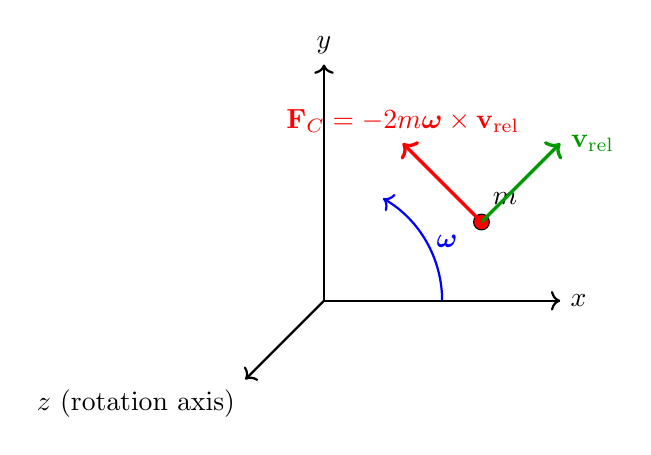
\begin{tikzpicture}[scale=1.0]
    \draw[->,thick] (0,0) -- (3,0) node[right] {$x$};
    \draw[->,thick] (0,0) -- (0,3) node[above] {$y$};
    \draw[->,thick] (0,0) -- (-1,-1) node[below left] {$z$ (rotation axis)};
    \draw[->,thick,blue] (1.5,0) arc (0:60:1.5) node[midway,right] {$\boldsymbol{\omega}$};
    \draw[fill=red] (2,1) circle (0.1);
    \node at (2.3,1.3) {$m$};
    \draw[->,very thick,green!60!black] (2,1) -- (3,2) node[right] {$\mathbf{v}_{\text{rel}}$};
    \draw[->,very thick,red] (2,1) -- (1,2) node[above] {$\mathbf{F}_C = -2m\boldsymbol{\omega} \times \mathbf{v}_{\text{rel}}$};
\end{tikzpicture}
\caption{Geometric relationship of Coriolis force.}
\label{fig:app_coriolis_force}
\end{figure}

\begin{figure}[H]
\centering
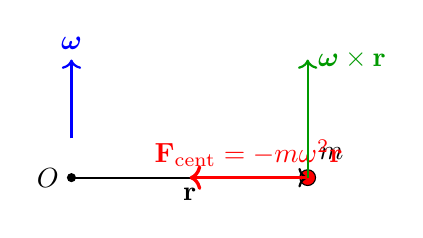
\begin{tikzpicture}[scale=1.0]
    \draw[fill=black] (0,0) circle (0.05);
    \node at (-0.3,0) {$O$};
    \draw[fill=red] (3,0) circle (0.1);
    \node at (3.3,0.3) {$m$};
    \draw[->,thick] (0,0) -- (3,0) node[midway,below] {$\mathbf{r}$};
    \draw[->,thick,blue] (0,0.5) -- (0,1.5) node[above] {$\boldsymbol{\omega}$};
    \draw[->,very thick,red] (3,0) -- (1.5,0) node[midway,above] {$\mathbf{F}_{\text{cent}} = -m\omega^2 \mathbf{r}$};
    \draw[->,thick,green!60!black] (3,0) -- (3,1.5) node[right] {$\boldsymbol{\omega} \times \mathbf{r}$};
\end{tikzpicture}
\caption{Centripetal force geometry.}
\label{fig:app_centripetal_force}
\end{figure}

\end{document}
